We test our stochastic trace estimator with both Chebyshev and Lanczos
approximation schemes on a variety of applications. Throughout we use the SKI
method \citep{wilson2015kernel} of \cref{eqn:ski} for fast MVMs. We find that
the Lanczos and surrogate methods are able to do kernel recovery and inference
significantly faster and more accurately than competing methods.

\subsection{Natural Sound Modeling}\label{sgpsec:sound}

Here we consider the natural sound benchmark in \cite{wilson2015kernel}, shown
in \cref{fig:sound_data}. Our goal is to recover contiguous missing
regions in a waveform with $N = 59,306$ training points. We exploit Toeplitz
structure in the $\K{UU}$ matrix of our SKI approximate kernel for accelerated
MVMs.

The experiment in \cite{wilson2015kernel} only considered scalable inference and
prediction, but not hyper\hyp{}parameter learning, since the scaled eigenvalue
approach requires all the eigenvalues for an $M \times M$ Toeplitz matrix, which
can be computationally prohibitive with cost $\calO(M^2)$. However, evaluating
the marginal likelihood on this training set is not an obstacle for Lanczos and
Chebyshev since we can use fast MVMs with the SKI approximation at a cost of
$\calO(N + M \log M)$.

In \cref{fig:sound_recovery}, we show how Lanczos, Chebyshev and surrogate
approaches scale with the number of inducing points $M$ compared to the scaled
eigenvalue method and FITC.  We use 5 probe vectors and 25 iterations for
Lanczos, both when building the surrogate and for hyper\hyp{}parameter learning
with Lanczos. We also use 5 probe vectors for Chebyshev and 100 moments. 
\cref{fig:sound_recovery} shows the runtime of the hyper\hyp{}parameter learning
phase for different numbers of inducing points $M$, where Lanczos and the
surrogate are clearly more efficient than scaled eigenvalues and Chebyshev. For
hyper\hyp{}parameter learning, FITC took several hours to run, compared to
minutes for the alternatives; we therefore exclude FITC from 
\cref{fig:sound_recovery}. \cref{fig:sound_inference} shows the time to do
inference on the 691 test points,while \ref{fig:sound_smae} shows the
standardized mean absolute error (SMAE) on the same test points. As expected,
Lanczos and surrogate make accurate predictions much faster than Chebyshev,
scaled eigenvalues, and FITC. In short, Lanczos and the surrogate approach are
much faster than alternatives for hyper\hyp{}parameter learning with a large
number of inducing points and training points.

\begin{figure}[ht]
  \begin{center}
    \begin{subfigure}{0.47\textwidth}
      \centering
      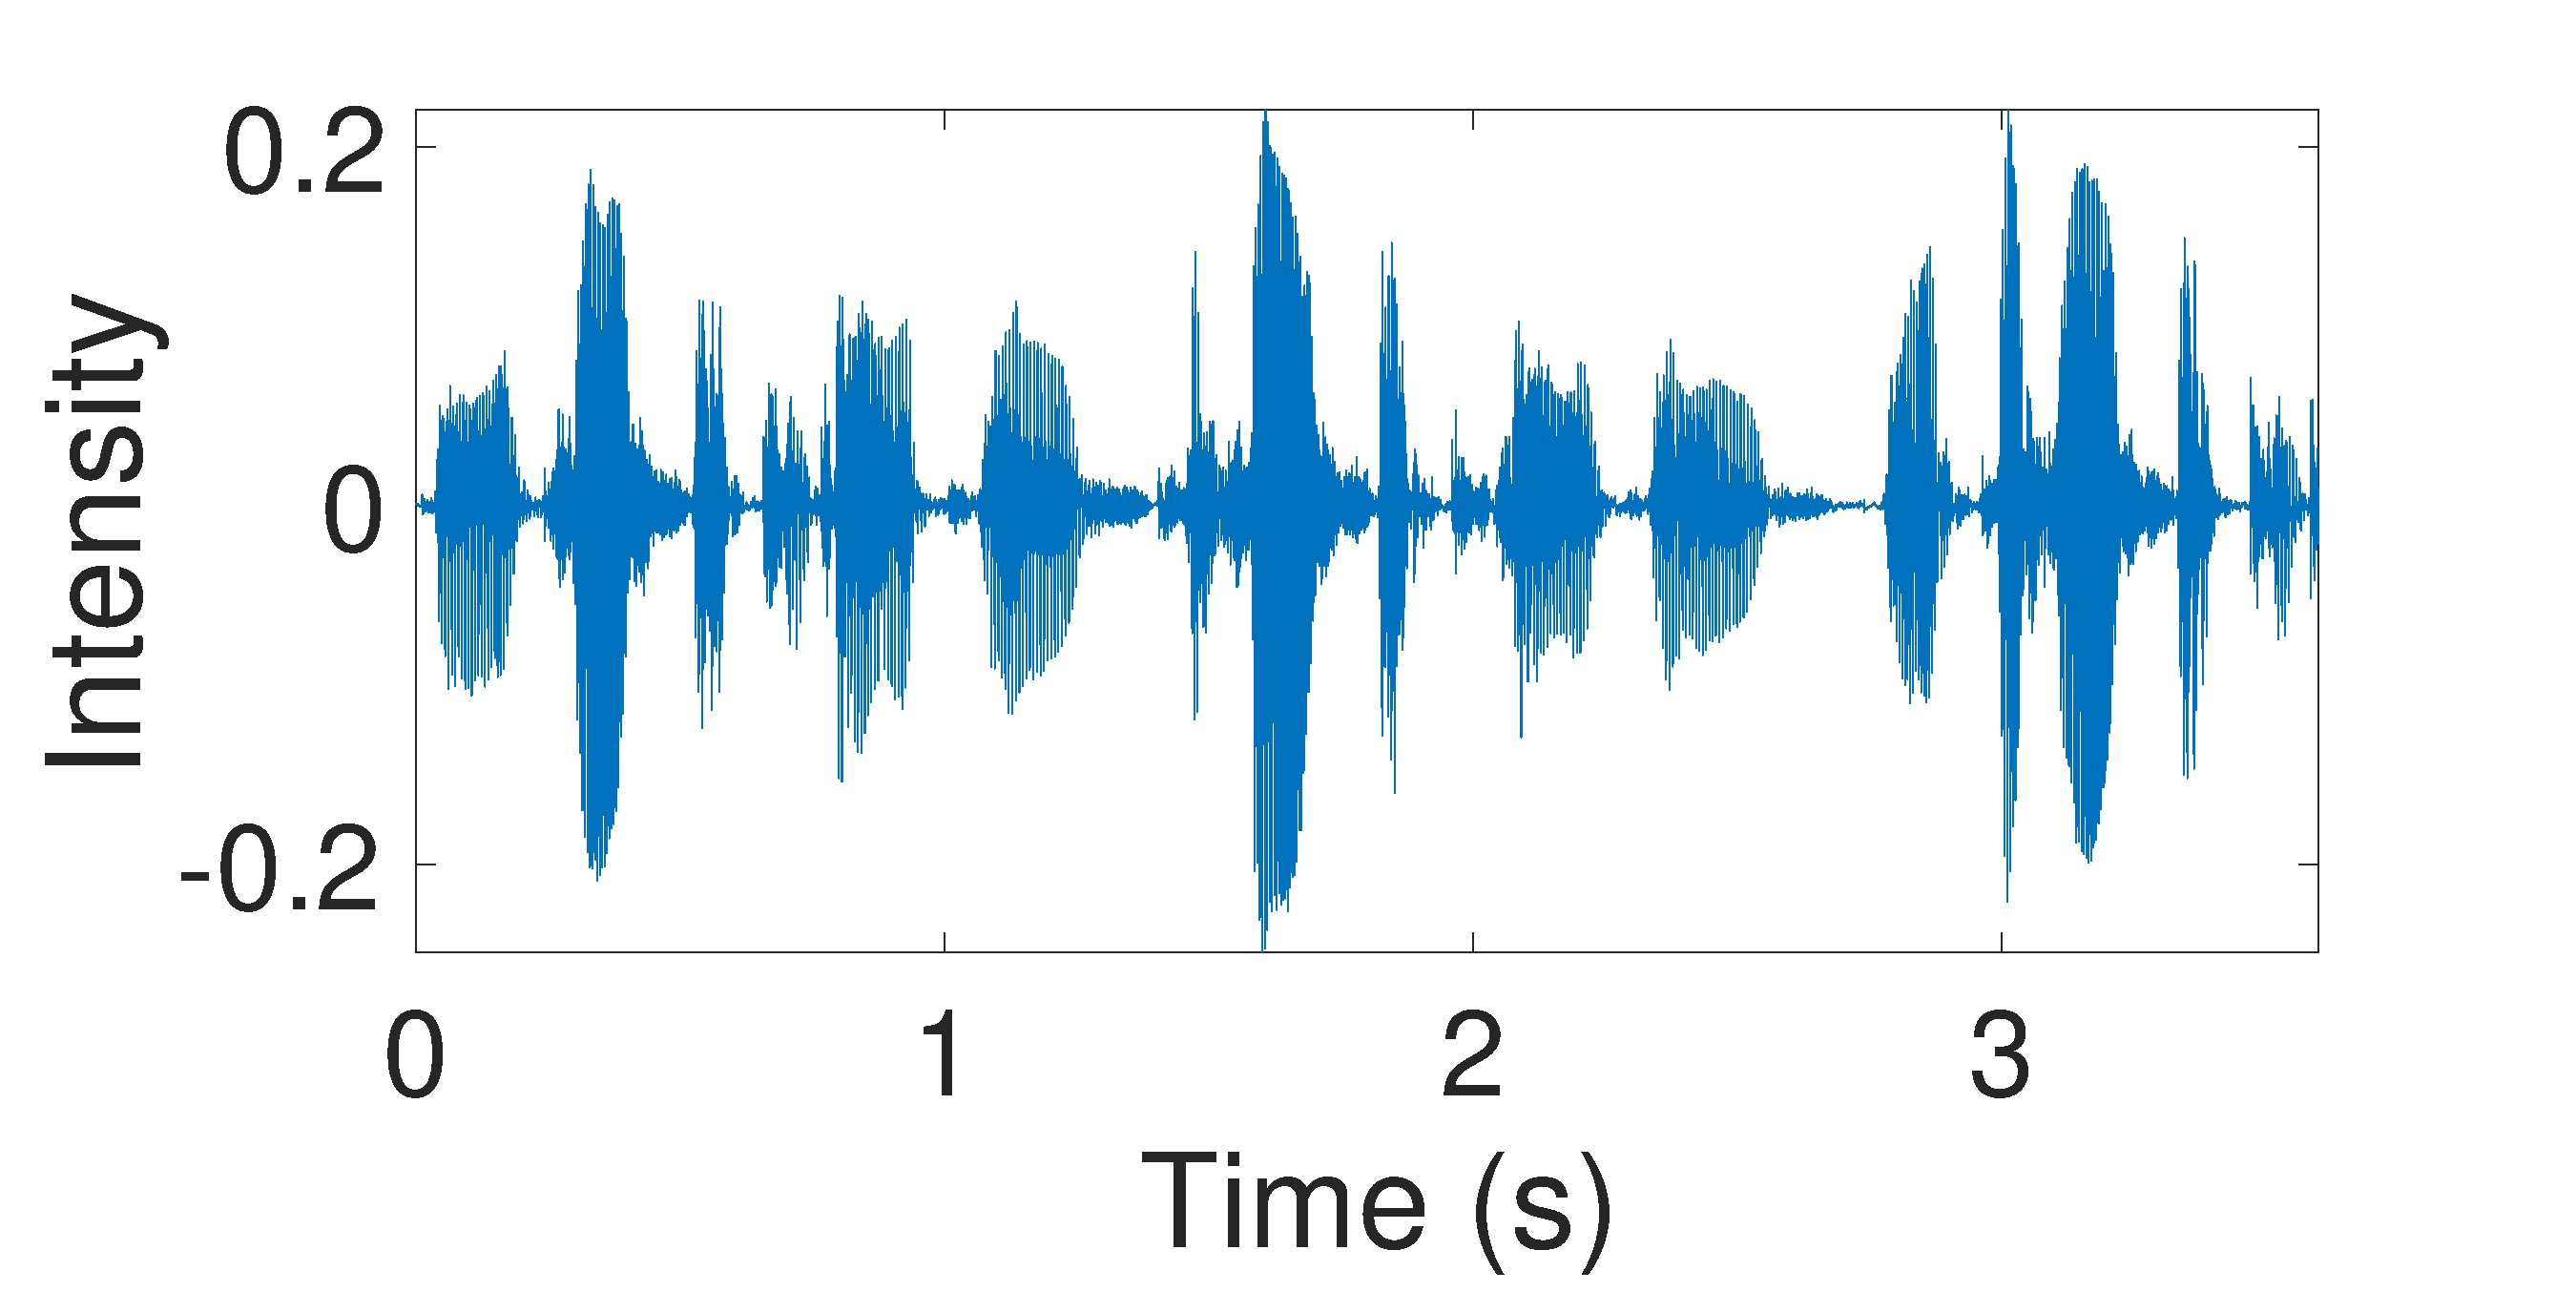
\includegraphics[width=\textwidth,trim=0.4cm 0cm 3.5cm 1.0cm,clip]
      {./sgp/pics/sound_data}
      \caption{Sound Data}
      \label{fig:sound_data}
    \end{subfigure}
    %
    \begin{subfigure}{0.47\textwidth}
      \centering
      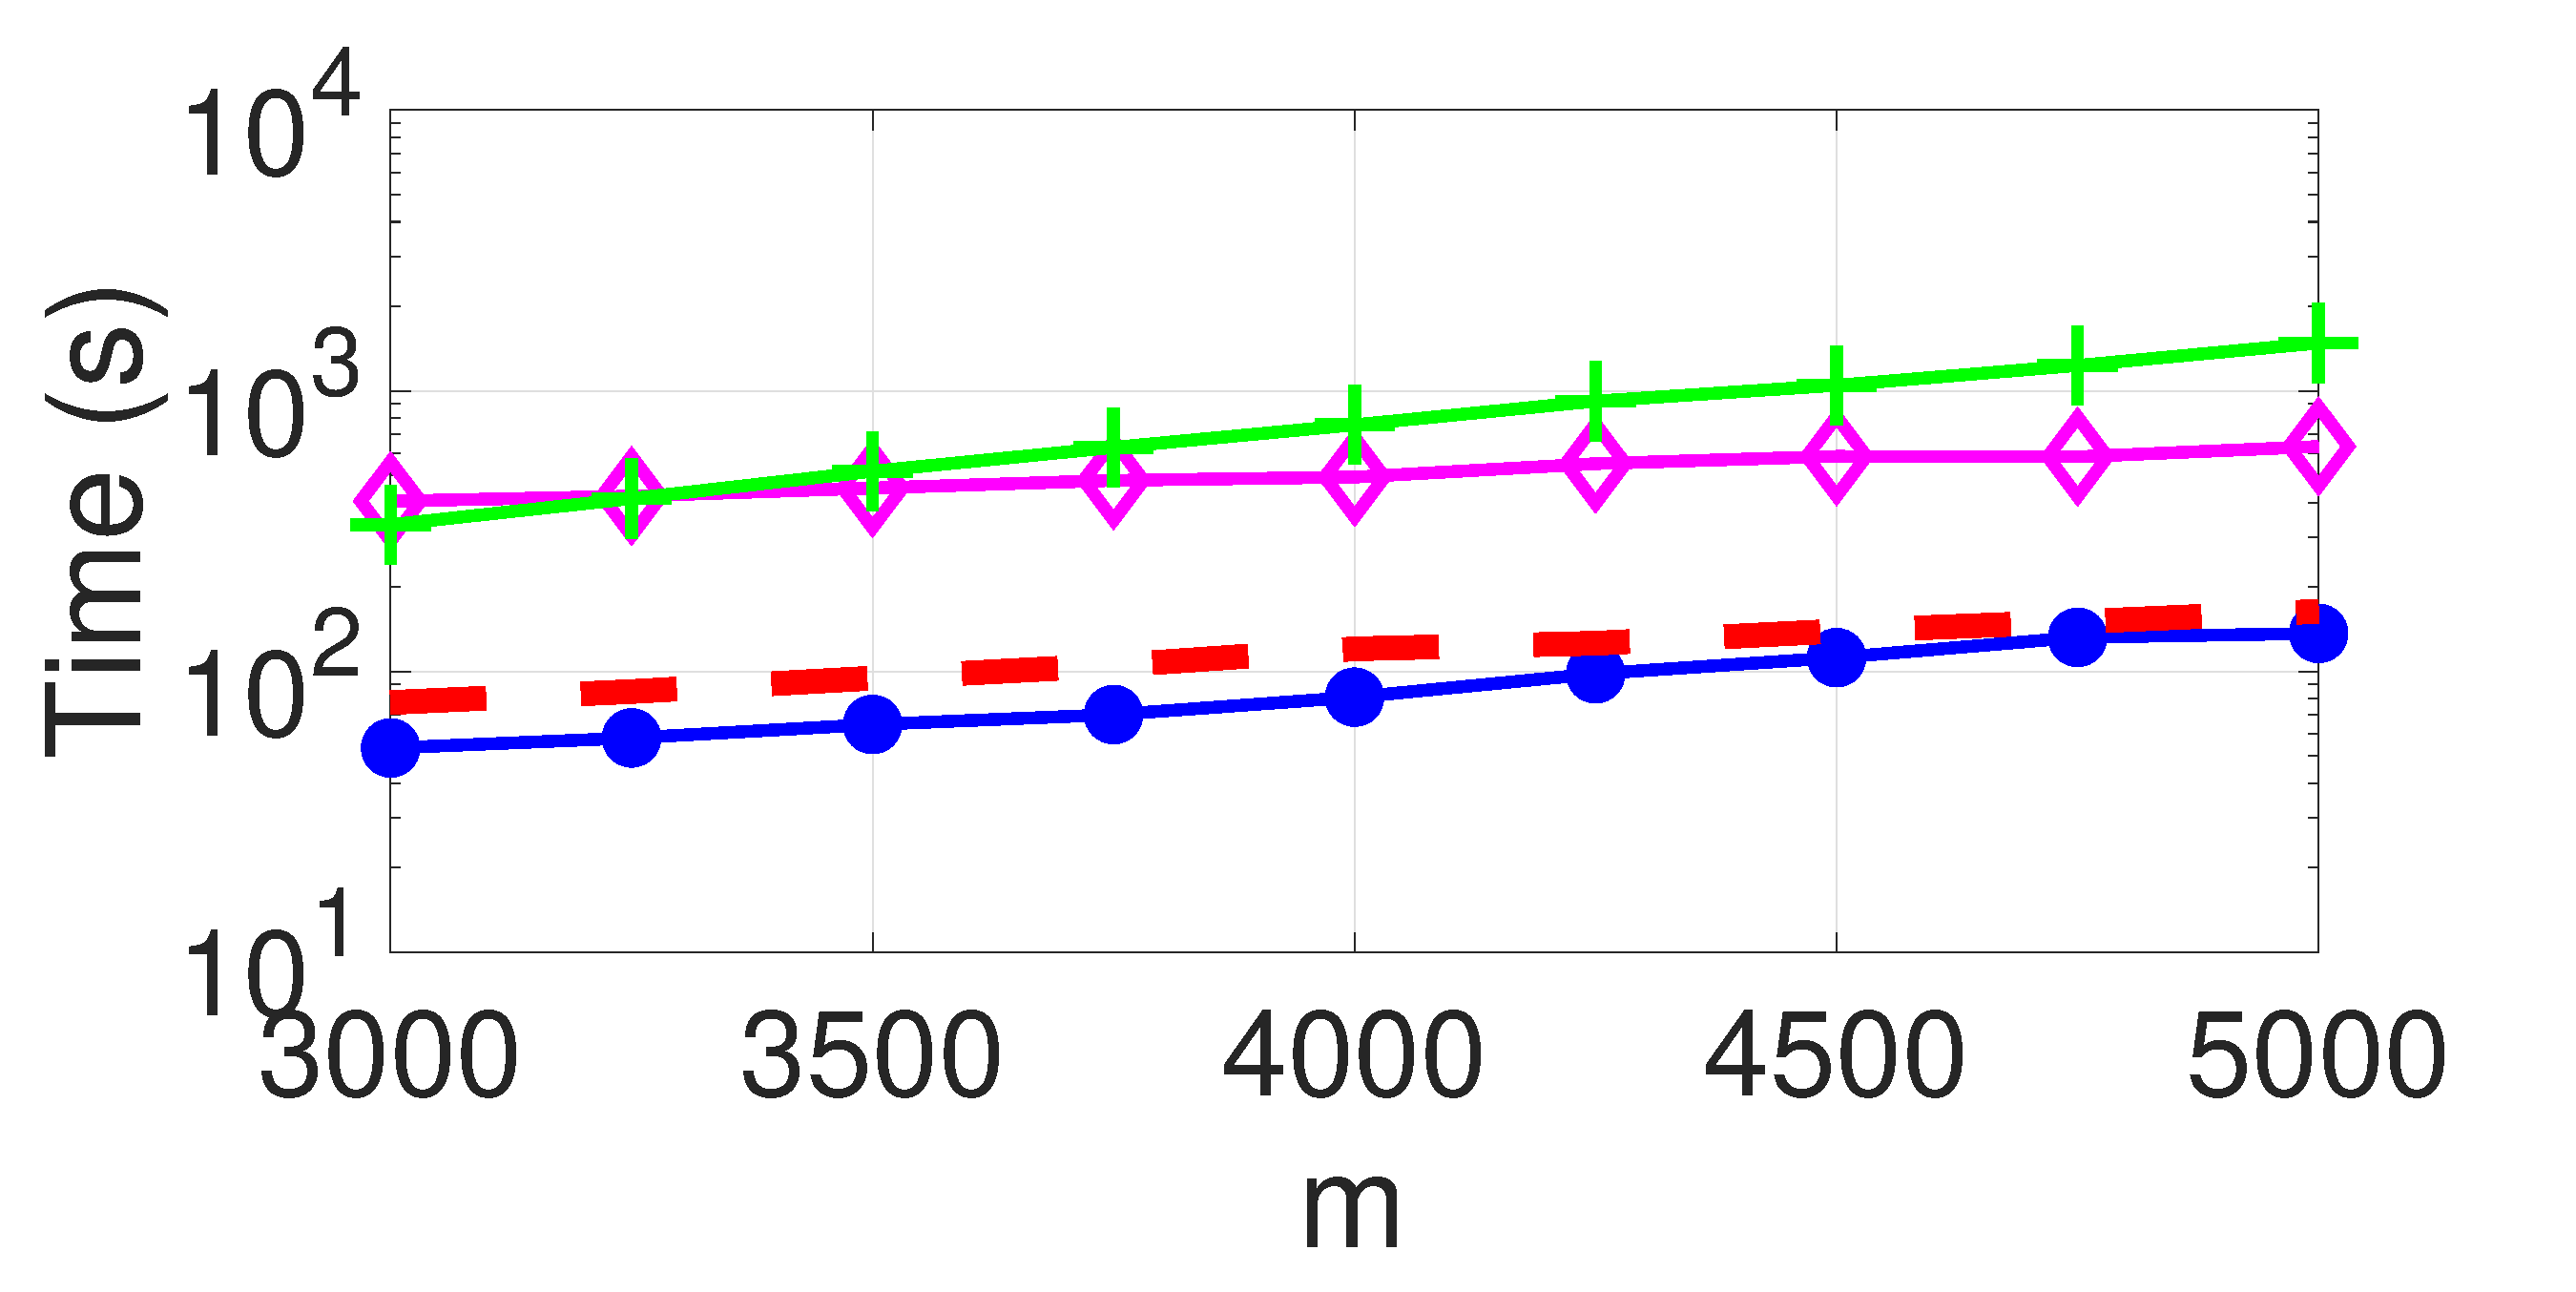
\includegraphics[width=\textwidth,trim=0.4cm 0cm 2.0cm 0cm,clip]
      {./sgp/pics/sound_recovery}
      \caption{Recovery Time}\label{fig:sound_recovery}
    \end{subfigure}
    %
    \begin{subfigure}{0.47\textwidth}
      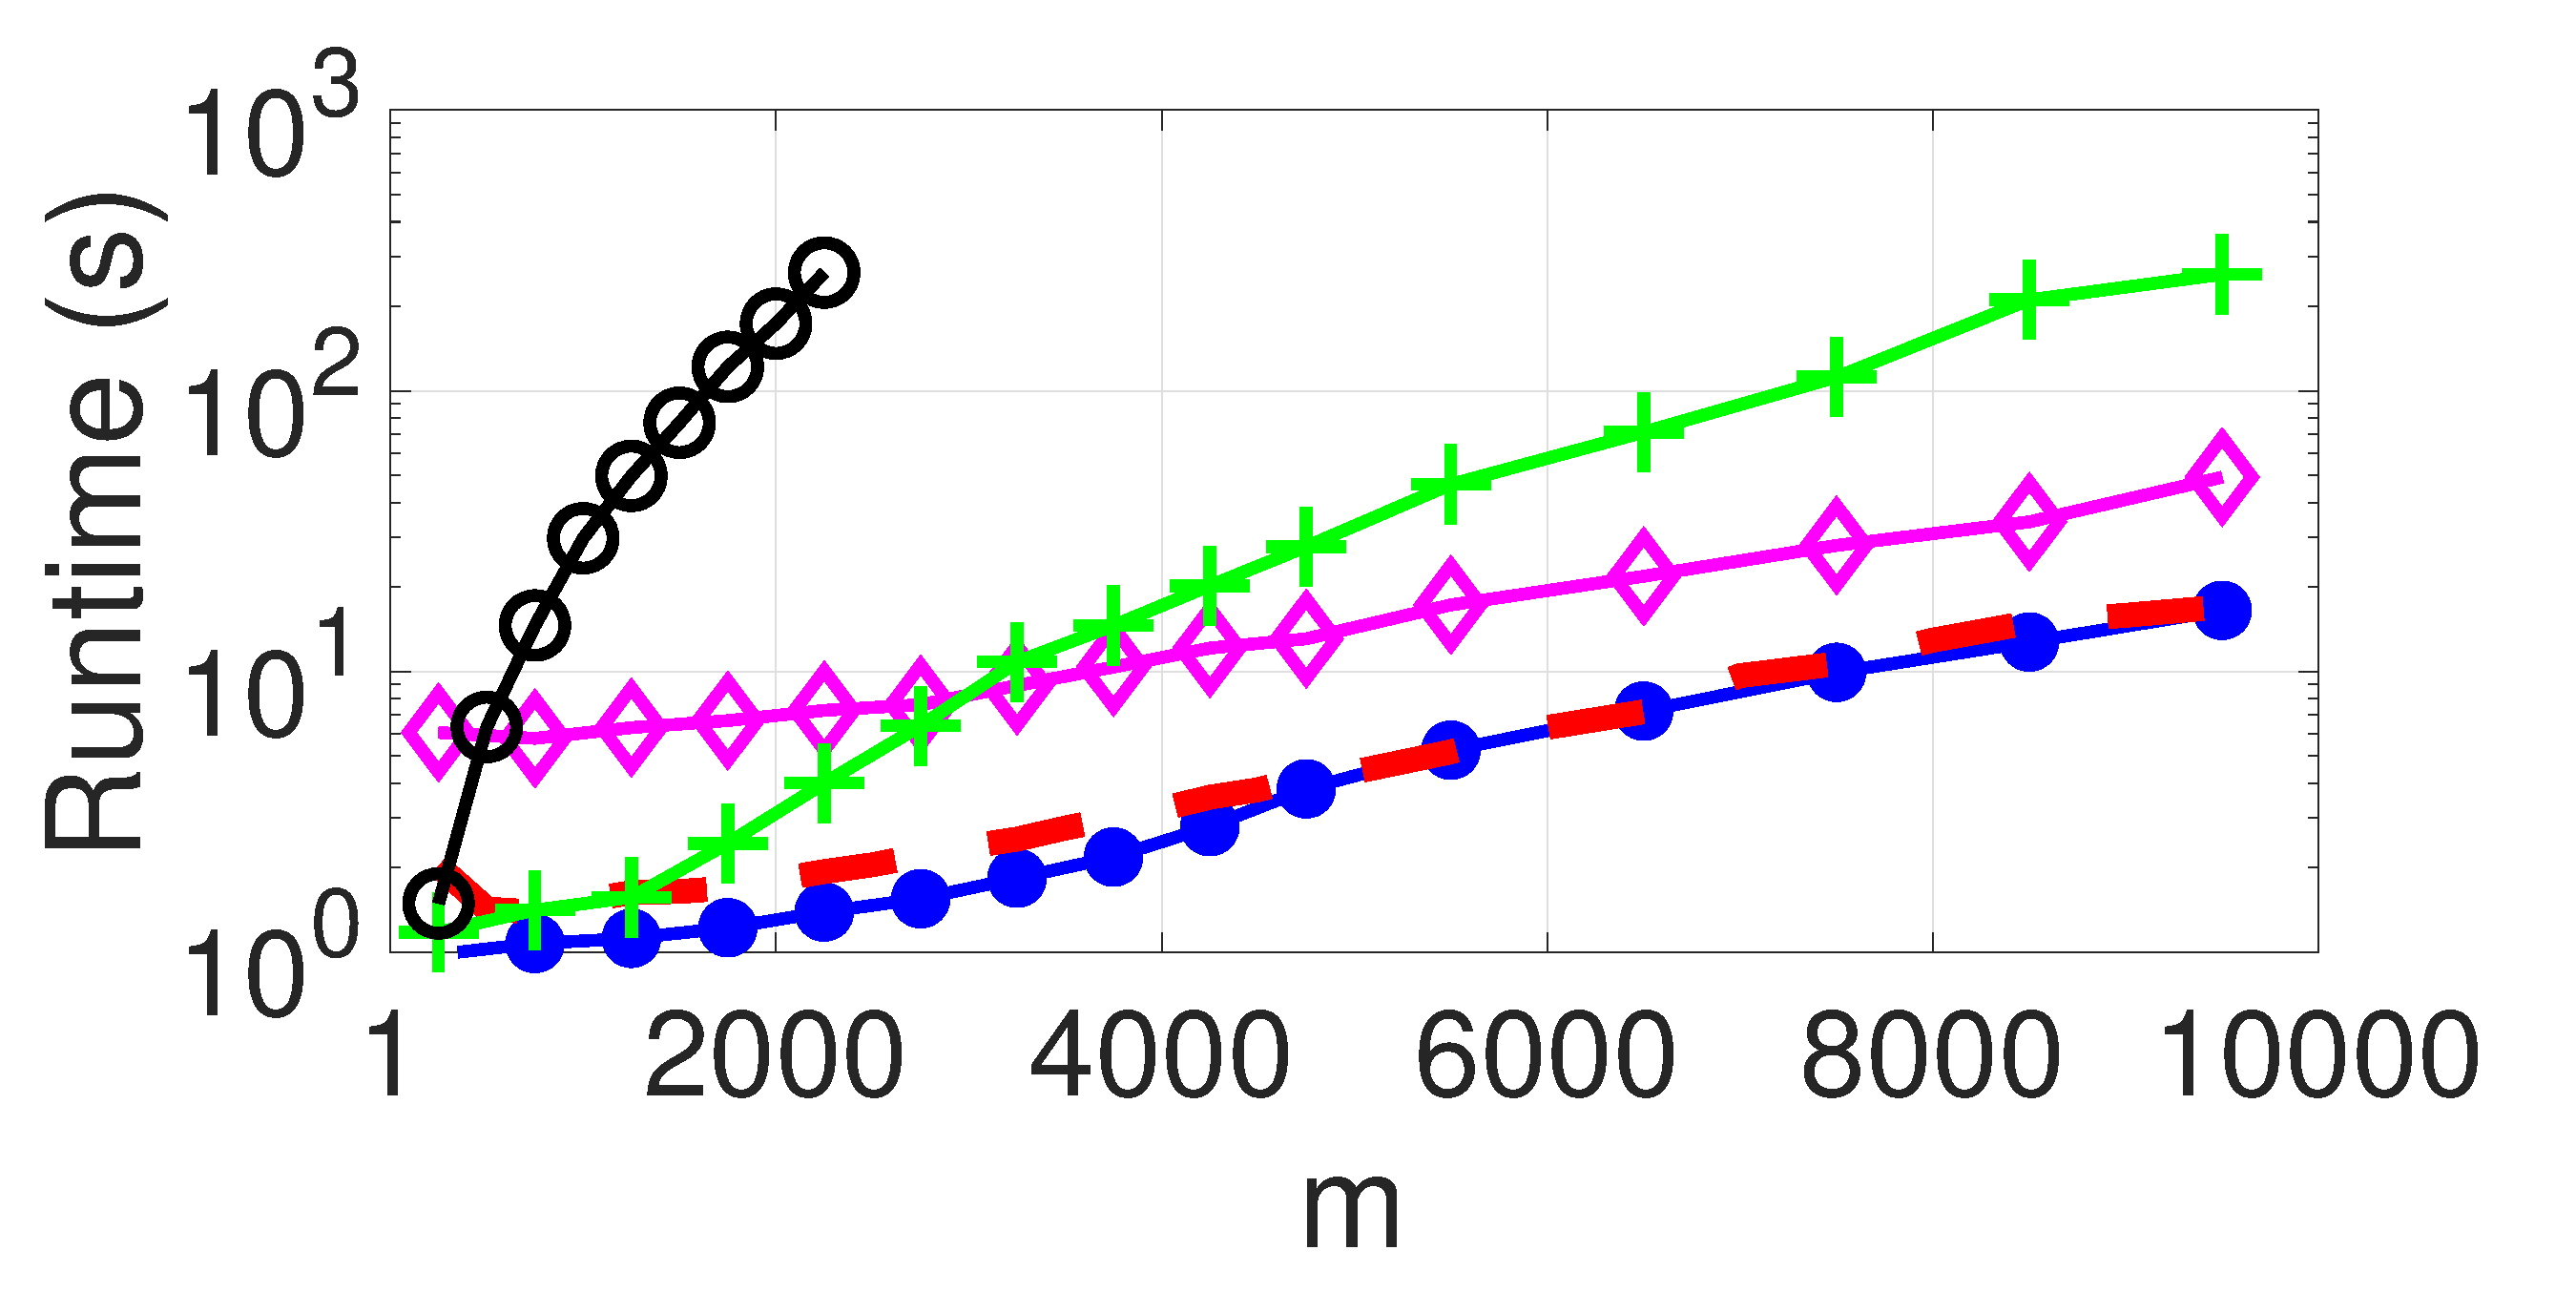
\includegraphics[width=\textwidth,trim=0.4cm 0cm 1.5cm 0.5cm,clip]
      {./sgp/pics/sound_inference}
      \caption{Inference Time}\label{fig:sound_inference}
    \end{subfigure}
    %
    \begin{subfigure}{0.47\textwidth}
      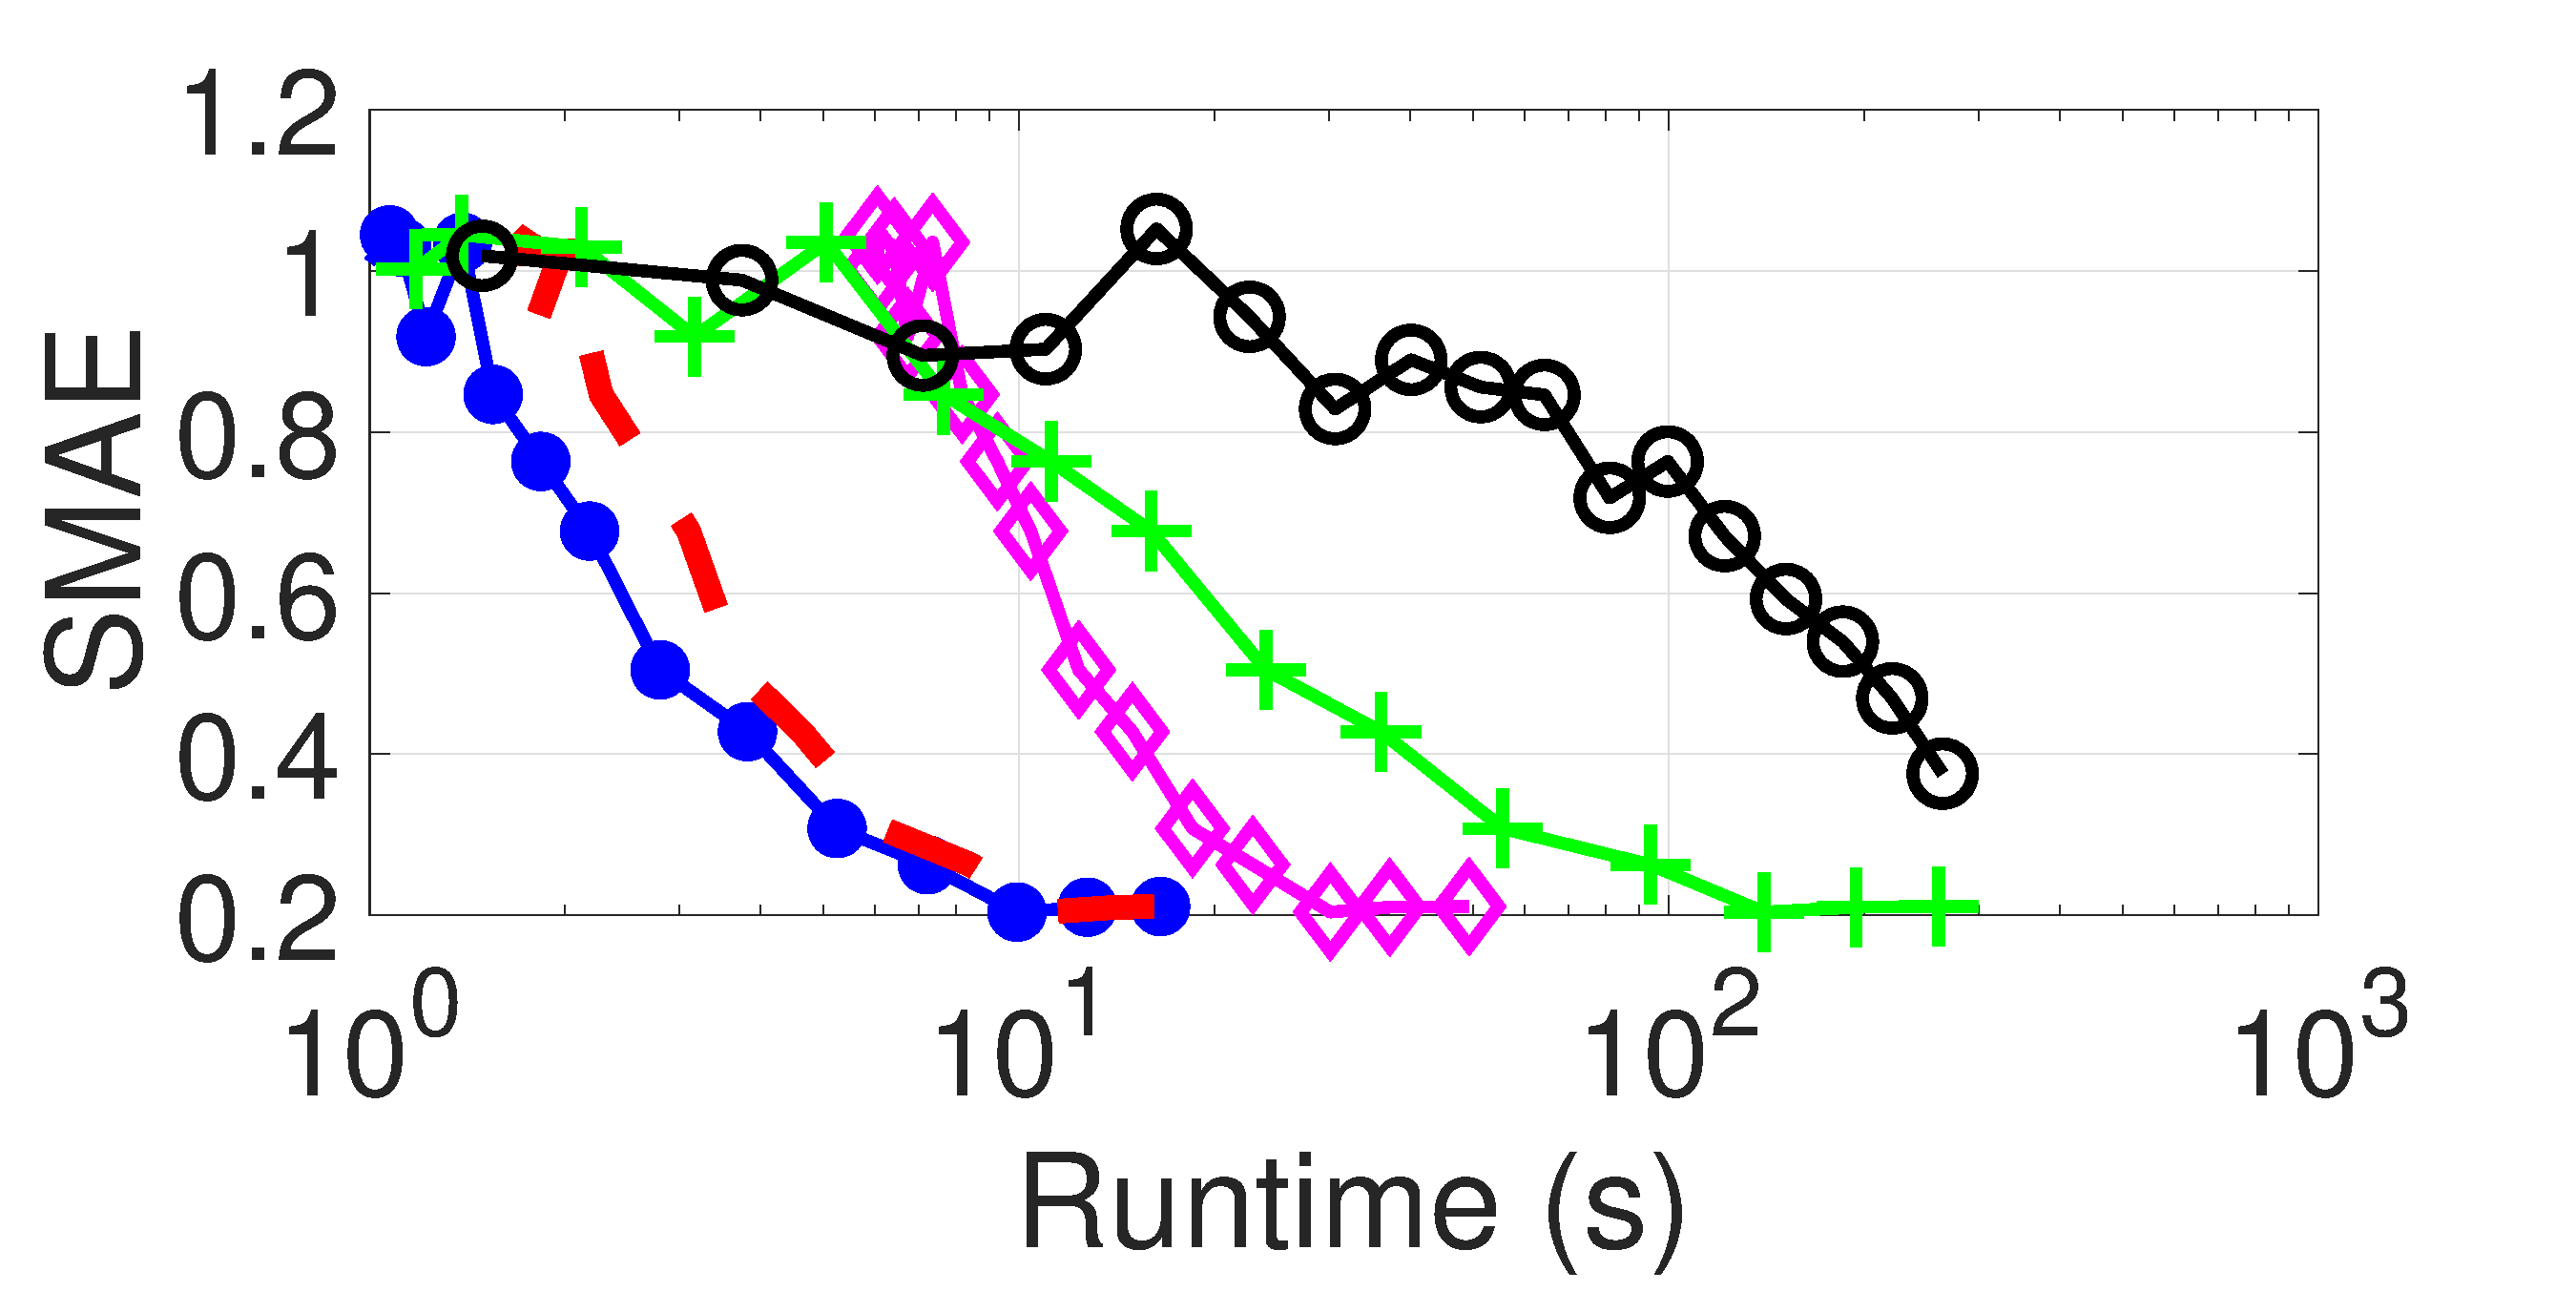
\includegraphics[width=\textwidth,trim=0.4cm 0cm 2.5cm 0.5cm,clip]
      {./sgp/pics/sound_smae}
      \caption{SMAE}\label{fig:sound_smae}
    \end{subfigure}
  \end{center}
  \caption{Sound modeling using 59,306 training points and 691 test points. The
  intensity of the time series can be seen in (a). Train time for RBF kernel
  hyper\hyp{}parameters is in (b) and the time for inference is in (c). The
  standardized mean absolute error (SMAE) as a function of time for an
  evaluation of the marginal likelihood and all derivatives is shown in (d).
  Surrogate is ({\color{blue} ------}), Lanczos is ({\color{red} - - -}),
  Chebyshev is {(\color{magenta} --- $\diamond$ ---}), scaled eigenvalues is ({
  \color{green} --- + ---}), and FITC is ({\color{black} --- o ---}).}
  \label{fig:sound_modeling}
\end{figure}

\subsection{Daily Precipitation Prediction}

This experiment involves precipitation data from the year of 2010 collected from
around $5500$ weather stations in the US\footnote{\url{https://catalog.data.gov/
dataset/u-s-hourly-precipitation-data}}. The hourly precipitation data is
preprocessed into daily data if full information of the day is available. The
dataset has $628,474$ entries in terms of precipitation per day given the date,
longitude and latitude. We randomly select $100,000$ data points as test points
and use the remaining points for training. We then perform hyper\hyp{}parameter
learning and prediction with the RBF kernel, using Lanczos, scaled eigenvalues,
and exact methods.

For Lanczos and scaled eigenvalues, we optimize the hyper\hyp{}parameters on the
subset of data for January 2010, with an induced grid of $100$ points per
spatial dimension and $300$ in the temporal dimension. Due to memory constraints
we only use a subset of $12,000$ entries for training with the exact method.
While scaled eigenvalues can perform well when fast eigendecompositions are
possible, as in this experiment, Lanczos nonetheless still runs faster and with
slightly lower mean square error (MSE).

\begin{table}[ht]
  \centering
  \caption{Prediction Comparison for the Daily Precipitation Data
  \textsuperscript{$\alpha$}.}\label{tab:precip}
  \begin{threeparttable}
    \begin{tabular}{r c c c c}
      \toprule
      Method  & \#Training Pts   & \#Induced Pts & MSE & Time [min]\\ \midrule
      Lanczos & 528k  & 3M  & 0.613 &  14.3\\
      Scaled\hyp{}Eig & 528k  & 3M  & 0.621 &  15.9\\
      Exact   & 12k   & -   & 0.903 &  11.8\\
      \bottomrule
    \end{tabular}
    \begin{tablenotes}
      \item[$\alpha$] The columns are the number of training points, number of
      induced grid points, mean squared error, and inference time.
    \end{tablenotes}
  \end{threeparttable}
\end{table}
Incidentally, we are able to use 3 \emph{million} inducing points in Lanczos and
scaled eigenvalues, which is enabled by the SKI representation 
\citep{wilson2015kernel} of covariance matrices, for a a very accurate
approximation.  This number of inducing points $M$ is unprecedented for typical
alternatives which scale as $\calO(M^3)$.

\subsection{Hickory Data}

In this experiment, we apply Lanczos to the log\hyp{}Gaussian Cox process model
with a Laplace approximation for the posterior distribution. We use the RBF
kernel and the Poisson likelihood in our model.  The scaled eigenvalue method
does not apply directly to non\hyp{}Gaussian likelihoods; we thus applied the
scaled eigenvalue method in \citep{wilson2015kernel} in conjunction with the
Fiedler bound in \citep{flaxman2015fast} for the scaled eigenvalue comparison. 
Indeed, a key advantage of the Lanczos approach is that it can be applied
whenever fast MVMs are available, which means no additional approximations such
as the Fiedler bound are required for non\hyp{}Gaussian likelihoods.

This dataset, which comes from the R package {\tt spatstat}, is a point pattern
of $703$ hickory trees in a forest in Michigan. We discretize the area into a
$60 \times 60$ grid and fit our model with exact, scaled eigenvalues, and
Lanczos. We see in Table \ref{tab:hickory} that Lanczos recovers
hyper\hyp{}parameters that are much closer to the exact values than the scaled
eigenvalue approach. \cref{fig:hickory} shows that the predictions by Lanczos
are also indistinguishable from the exact computation.

\begin{table}[ht]
  \centering
  \caption{Hyperparameters Recovered on the Hickory Dataset.}\label{tab:hickory}
  \begin{tabular}{r c c c c c}
    \toprule
    Method & $s_f$ & $\ell_1$ & $\ell_2$ & $-\log p(y|\theta)$ & Time [s]\\
    \midrule
    Exact & $0.696$  & $0.063$  & $0.085$ &  $1827.56$ & $465.9$\\
    Lanczos & $0.693$   & $0.066$   & $0.096$ &  $1828.07$ & $21.4$\\
    Scaled\hyp{}Eig & $0.543$  & $0.237$  & $0.112$ &  $1851.69$ & $2.5$\\
    \bottomrule
  \end{tabular}
\end{table}
\vfill

\begin{figure}[ht]
  \begin{center}
    \begin{subfigure}{0.3\textwidth}
      \centering
      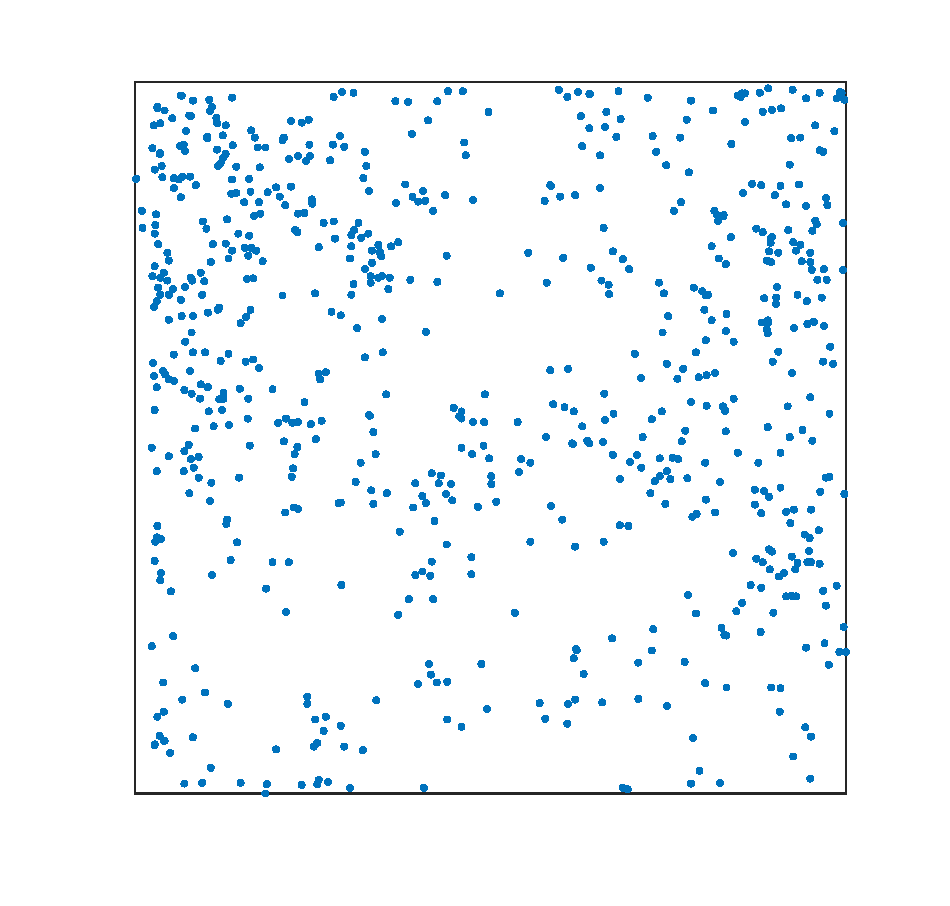
\includegraphics[height=0.87\textwidth,trim = 1cm 1cm 1cm 1cm,clip]
      {./sgp/pics/Hickory_point.eps}
      \caption{Point Pattern Data}\label{fig:hpoint}
    \end{subfigure}
    \hspace{1cm}
    \begin{subfigure}{0.3\textwidth}
      \centering
      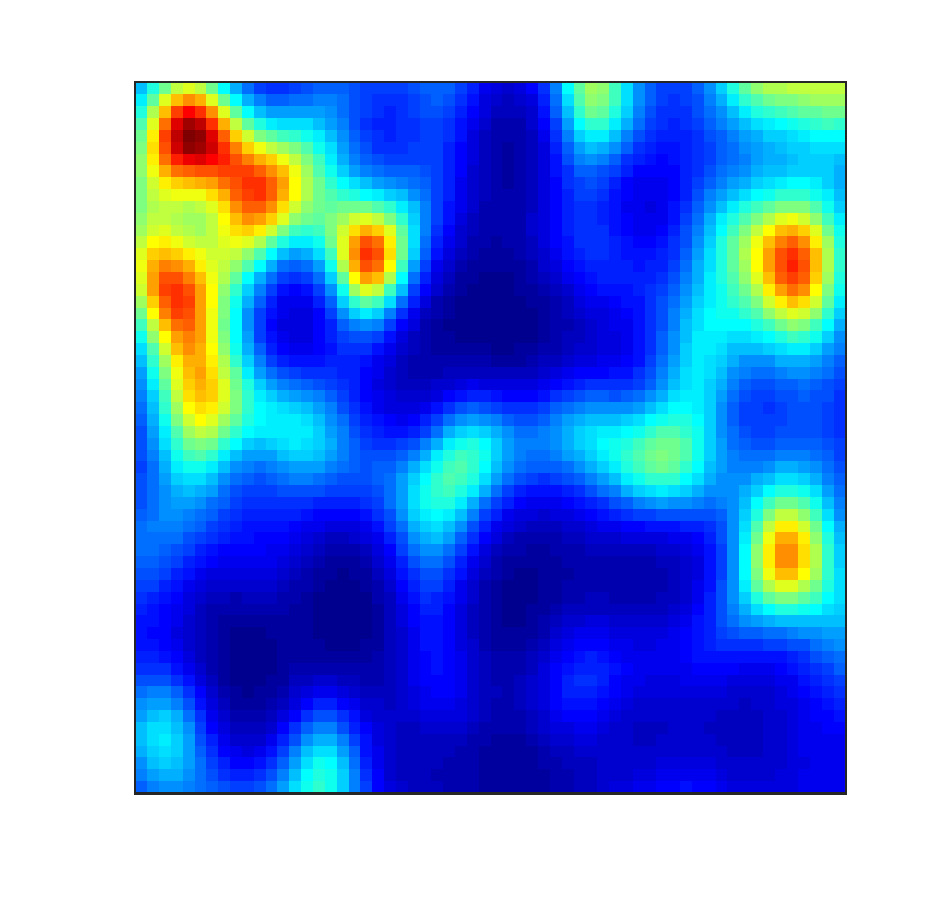
\includegraphics[height=0.87\textwidth,trim = 1cm 1cm 1cm 1cm,clip]
      {./sgp/pics/Hickory_exact.eps}
      \caption{Prediction by Exact}\label{fig:hickory_exact}
    \end{subfigure}
    \linebreak
    \begin{subfigure}{0.3\textwidth}
      \centering
      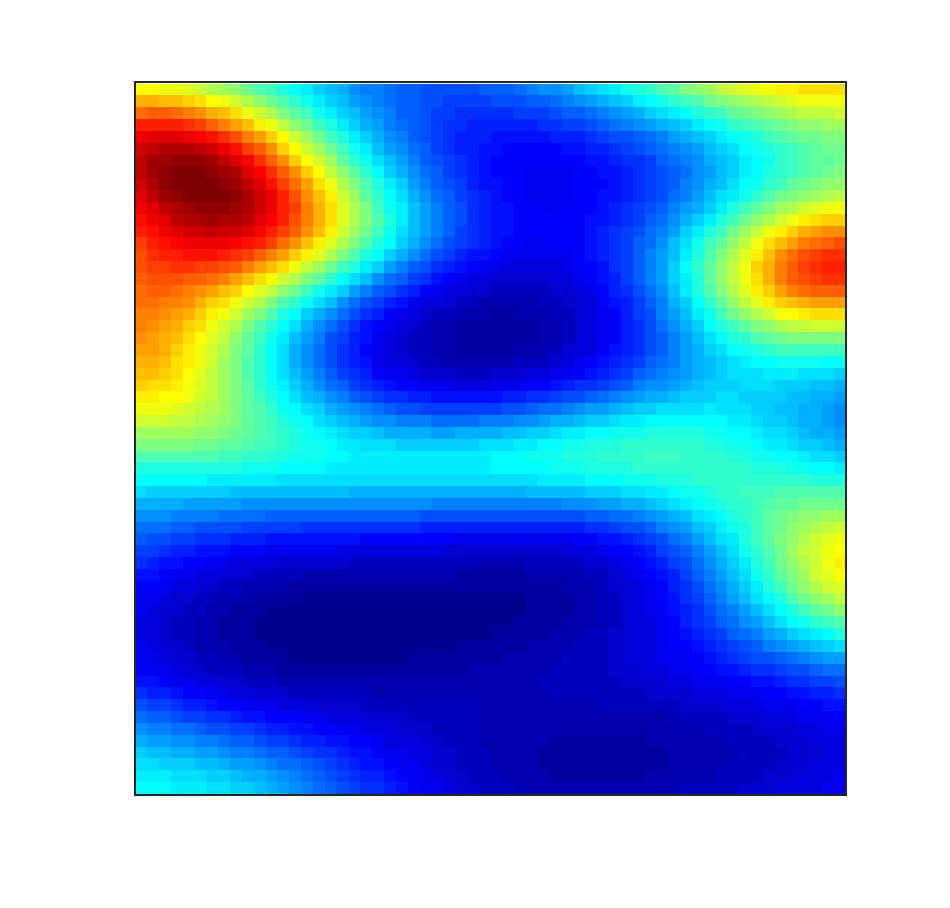
\includegraphics[height=0.87\textwidth,trim = 1cm 1cm 1cm 1cm,clip]
      {./sgp/pics/Hickory_ski.eps}
      \caption{Scaled\hyp{}Eig}\label{fig:hickory_ski}
    \end{subfigure}
    \hspace{1cm}
    \begin{subfigure}{0.3\textwidth}
      \centering
      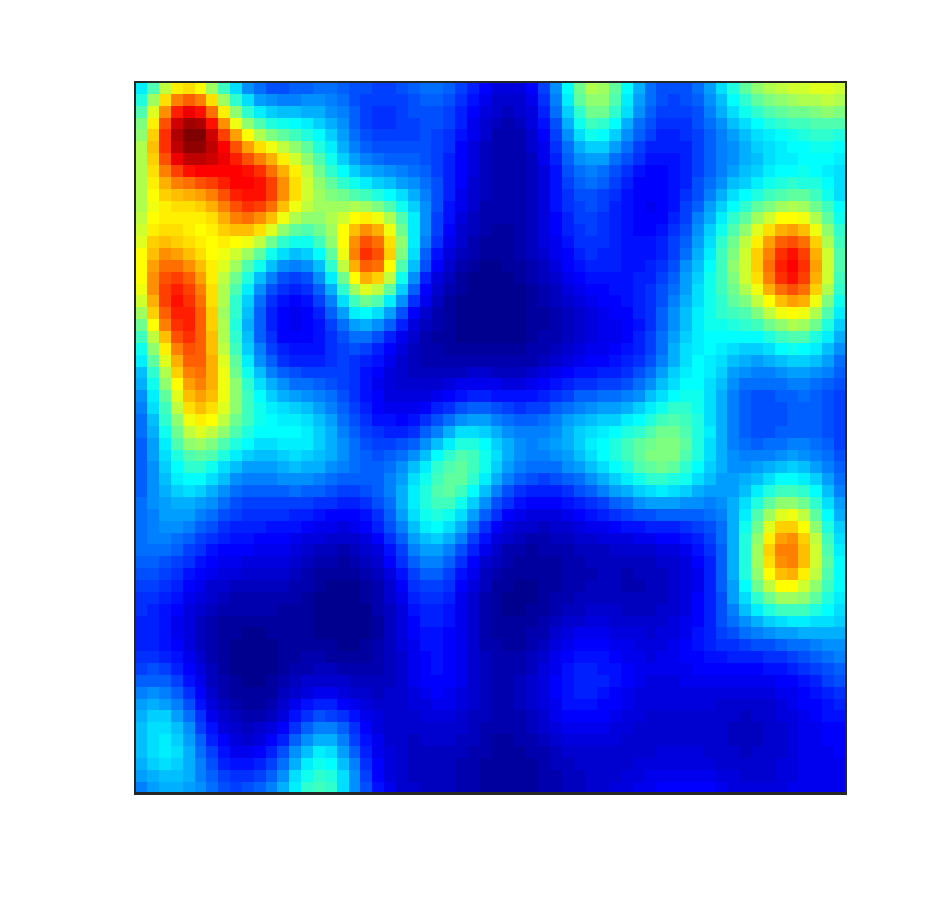
\includegraphics[height=0.87\textwidth,trim = 1cm 1cm 1cm 1cm,clip]
      {./sgp/pics/Hickory_lan.eps}
      \caption{Lanczos}\label{fig:hickory_lan}
    \end{subfigure}
    \caption{Predictions by exact, scaled eigenvalues, and Lanczos on the Hickory dataset.}\label{fig:hickory}
  \end{center}
\end{figure}

\subsection{Crime Prediction}

In this experiment, we apply Lanczos with the spectral mixture kernel to the
crime forecasting problem considered in \cite{flaxman2015fast}. This dataset
consists of $233,088$ incidents of assault in Chicago from January 1, 2004 to
December 31, 2013. We use the first $8$ years for training and attempt to
predict the crime rate for the last $2$ years. For the spatial dimensions, we
use the log\hyp{}Gaussian Cox process model, with the Mat\'ern\hyp{}5/2 kernel,
the negative binomial likelihood, and the Laplace approximation for the
posterior. We use a spectral mixture kernel with $20$ components and an extra
constant component for the temporal dimension. We discretize the data into a $17
\times 26$ spatial grid corresponding to $1\mile\Times1\mile$ grid cells. In
the temporal dimension we sum our data by weeks for a total of $522$ weeks.
After removing the cells that are outside Chicago, we have a total of $157,644$
observations.

The results for Lanczos and scaled eigenvalues (in conjunction with the Fiedler
bound due to the non\hyp{}Gaussian likelihood) can be seen in 
\cref{tab:chicago_homicide}. The Lanczos method used $5$ Hutchinson probe vectors
and $30$ Lanczos steps. For both methods we allow $100$ iterations of LBFGS to
recover hyper\hyp{}parameters and we often observe early convergence. While the
root mean square error (RMSE) for Lanczos and scaled eigenvalues happen to be
close on this example, the recovered hyper\hyp{}parameters using scaled
eigenvalues are very different than for Lanczos. For example, the scaled
eigenvalue method learns much larger $\sigma^2$ than Lanczos, indicating model
misspecification. In general, as the data become increasingly non\hyp{}Gaussian
the Fiedler bound (used for fast scaled eigenvalues on non\hyp{}Gaussian
likelihoods) will become increasingly misspecified, while Lanczos will be
unaffected.

\begin{table}[ht]
  \centering
  \caption{Hyperparameters Recovered, Recovery Time and RMSE for Lanczos and
  Scaled Eigenvalues on the Chicago Assault Data\textsuperscript{$\alpha$}.}
  \label{tab:chicago_homicide}
  \begin{threeparttable}
    \begin{tabular}{r c c c c c c c}
      \toprule
      Method & $\ell_1$ & $\ell_2$ & $\sigma^2$ & T\textsubscript{recovery}[s]&
      T\textsubscript{prediction}[s] & RMSE\textsubscript{train} &
      RMSE\textsubscript{test} \\
      \midrule
      Lanczos & 0.65 & 0.67 & \ph69.72 & 264 & 10.30 & 1.17 & 1.33 \\
      Scaled\hyp{}Eig & 0.32 & 0.10 & 191.17 & \ph67 & \ph3.75 & 1.19 & 1.36 \\
      \bottomrule
    \end{tabular}
    \begin{tablenotes}
      \item[$\alpha$] $\ell_1$ and $\ell_2$ are the length scales in
      spatial dimensions. $\sigma^2$ is the noise level.
      T\textsubscript{recovery} is the time for recovering hyper
      \hyp{}parameters. T\textsubscript{prediction} is the time for prediction
      at all $157,644$ observations, including training and testing.
    \end{tablenotes}
  \end{threeparttable} 
\end{table}

\subsection{Deep Kernel Learning}
To handle high\hyp{}dimensional datasets, we bring our methods into the deep
kernel learning framework \cite{wilson2016deep} by replacing the final layer of
a pre\hyp{}trained deep neural network (DNN) with a GP. This experiment uses the
gas sensor dataset from the UCI machine learning repository. It has $2565$
instances with $128$ dimensions. We pre\hyp{}train a DNN, then attach a Gaussian
process with RBF kernels to the two\hyp{}dimensional output of the
second\hyp{}to\hyp{}last layer. We then further train all parameters of the
resulting kernel, \emph{including} the weights of the DNN, through the GP
marginal likelihood. In this example, Lanczos and the scaled eigenvalue approach
perform similarly well.  Nonetheless, we see that Lanczos can effectively be
used with SKI on a high dimensional problem to train hundreds of thousands of
kernel parameters.

\begin{table}[ht]
  \centering
  \caption{Prediction RMSE and Per Training Iteration Runtime.}\label{tab:dkl}
  \begin{tabular}{r c c c}
    \toprule
    Method & DNN & Lanczos & Scaled\hyp{}Eig \\
    \midrule
    RMSE & $0.1366\pm 0.0387$ & $0.1053\pm0.0248$ & $0.1045\pm 0.0228$\\
    Time [s]& $0.4438$ & $2.0680$ & $1.6320$\\
    \bottomrule
  \end{tabular} 
\end{table}

\subsection{1D Cross-section Plots}\label{sup:1dcross}

In this experiment we compare the accuracy of Lanczos and Chebyshev for
1\hyp{}dimensional perturbations of a set of true hyper\hyp{}parameters,
and demonstrate how critical it is to use diagonal replacement for some
approximate kernels. We choose the true hyper\hyp{}parameters to be $
(\ell,s_f,\sigma) = (0.1,1,0.1)$ and consider two different types of datasets.
The first dataset consists of $1000$ equally spaced points in the interval $
[0,4]$ in which case the kernel matrix of a stationary kernel is Toeplitz and we
can make use of fast matrix\hyp{}vector multiplication. The second dataset
consists of $1000$ data points drawn independently from a
$U(0,4)$ distribution. We use SKI with cubic interpolation to construct an
approximate kernel based on $1000$ equally spaced points. The function values
are drawn from a GP with the true hyper\hyp{}parameters, for both the true and
approximate kernel. We use $250$ iterations for Lanczos and $250$ Chebyshev
moments in order to assure convergence of both methods. The results for the
first dataset with the RBF and Mat\'ern kernels can be seen in 
\crefrange{fig:1dpert_a}{fig:1dpert_d}. The results for the second
dataset with the SKI kernel can be seen in 
\crefrange{fig:1dpert_kissgp_a}{fig:1dpert_kissgp_d}.

\begin{figure}[ht]
  \begin{center}
    \begin{subfigure}{0.46\textwidth}
      \centering
      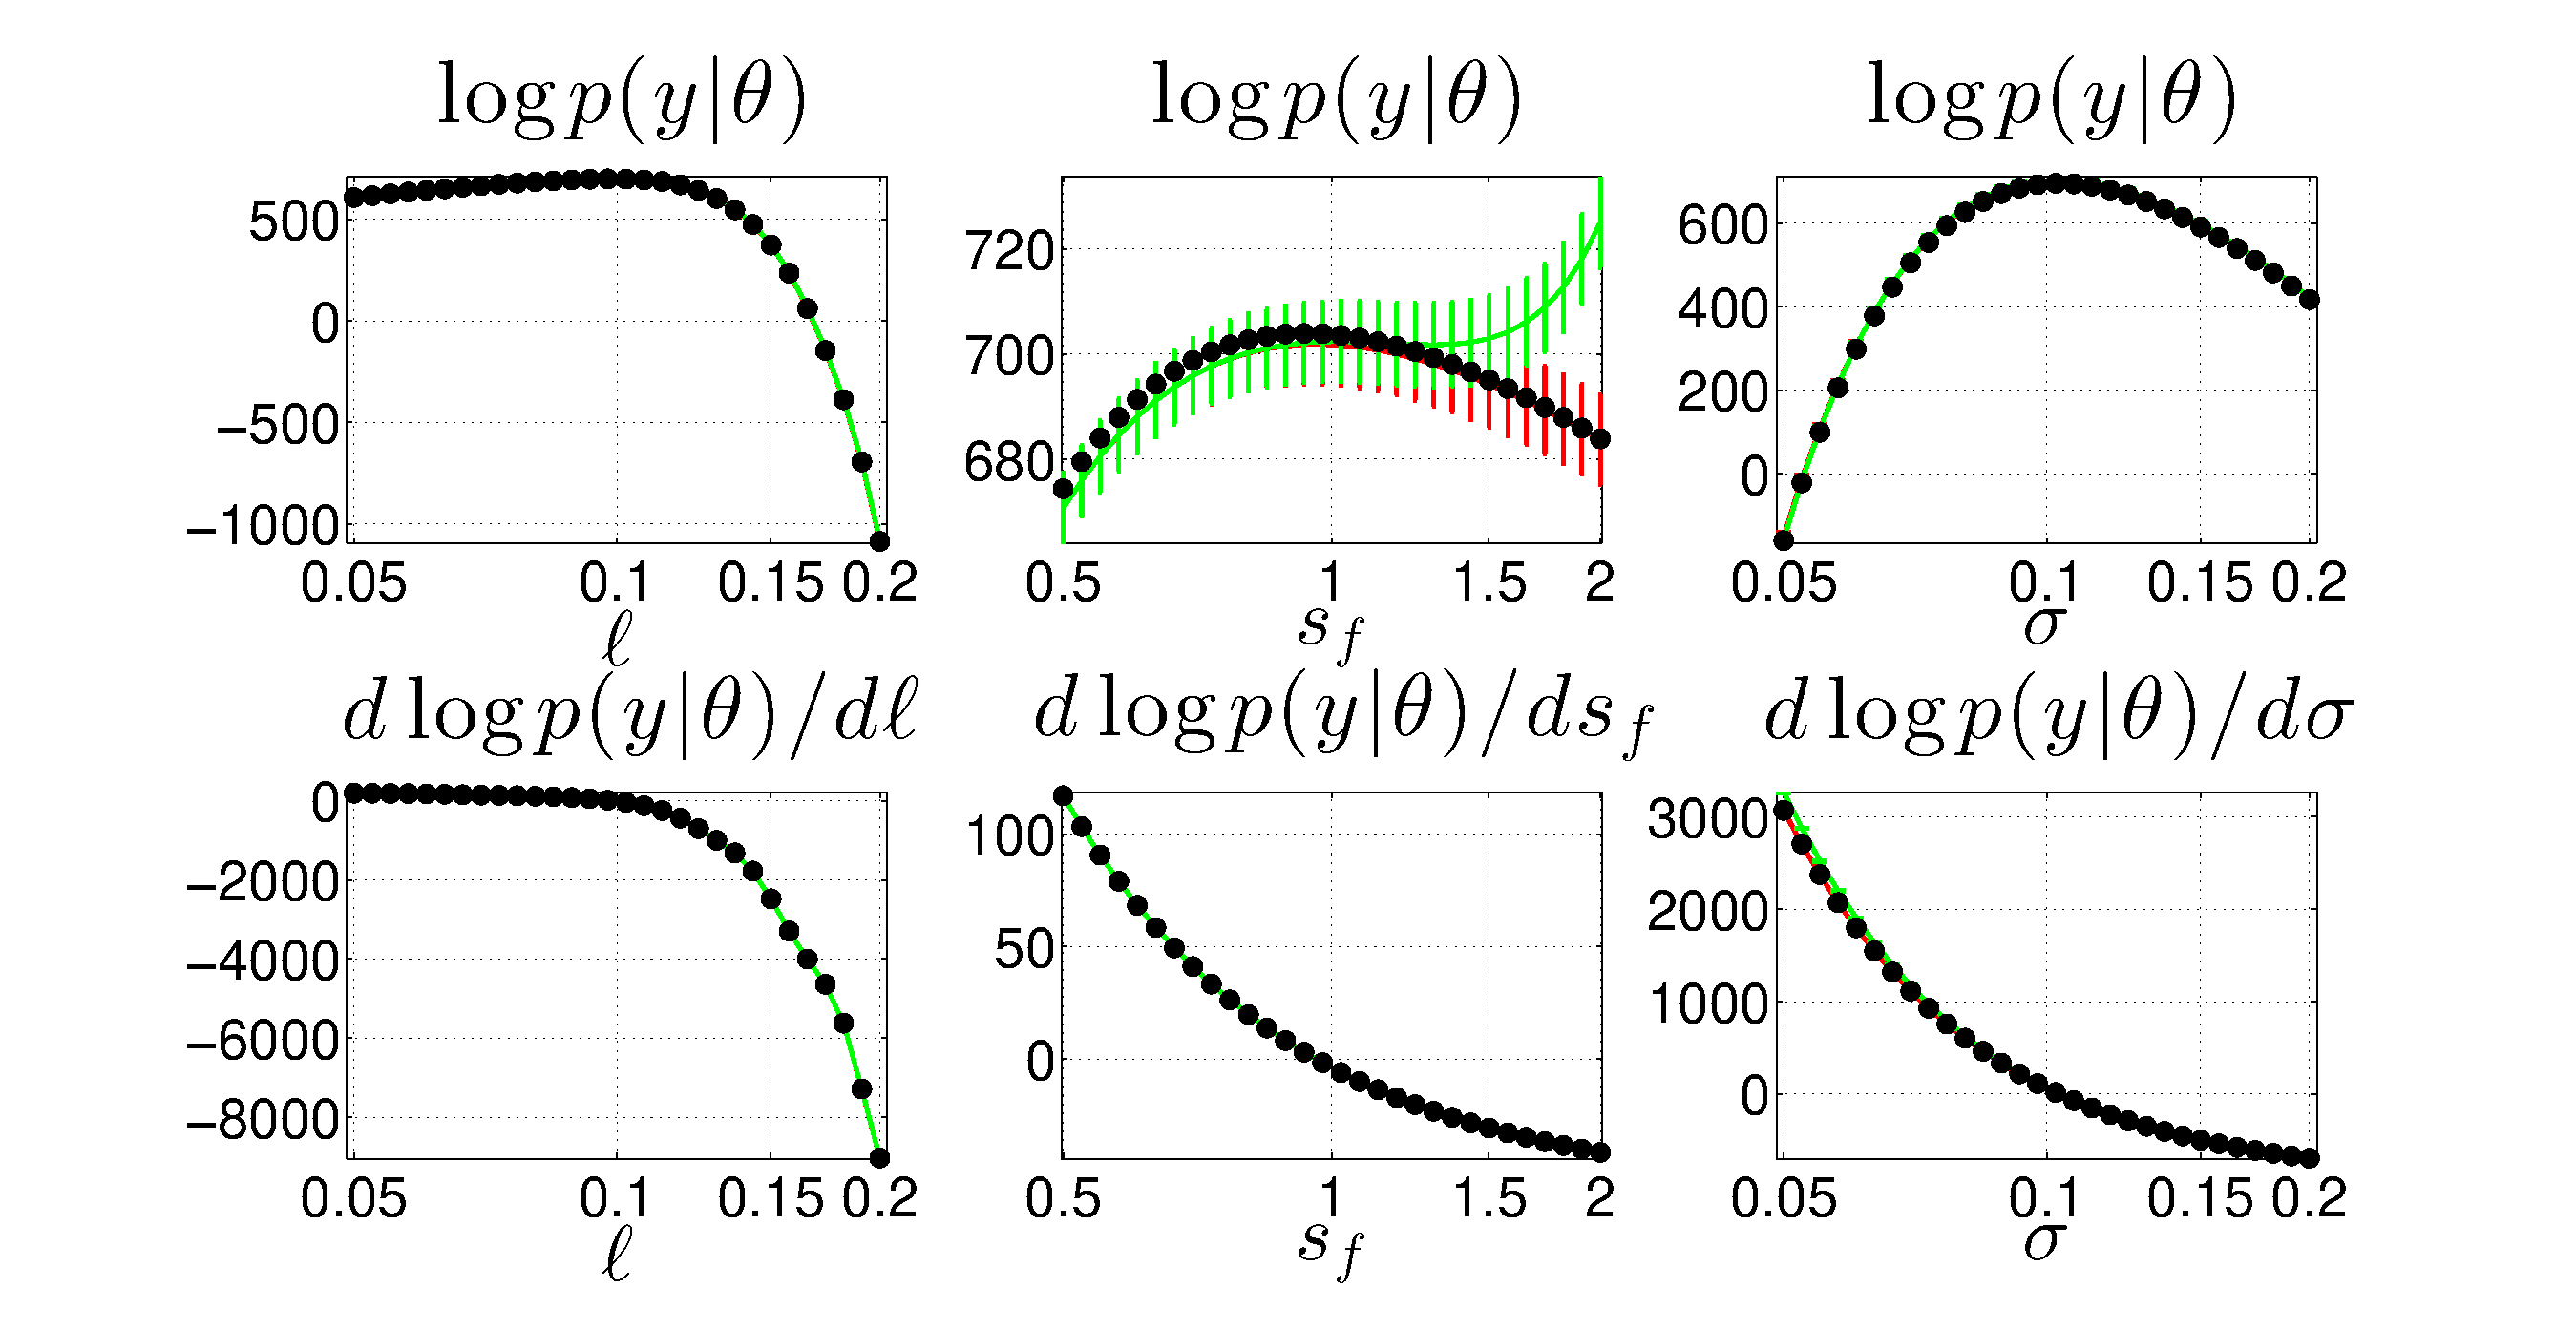
\includegraphics[width=\textwidth,trim=3.5cm 0cm 3.5cm 0cm,clip]
      {./sgp/pics/loglik_rbf}
      \caption{Log marginal likelihood for the RBF \\kernel}\label{fig:1dpert_a}
    \end{subfigure}
    \begin{subfigure}{0.46\textwidth}
      \centering
      \includegraphics[width=\textwidth,trim=3.5cm 0cm 3.5cm 0cm,clip]
      {./sgp/pics/loglik_Matern}
      \caption{Log marginal likelihood for the Mat\'ern \\kernel}
      \label{fig:1dpert_b}
    \end{subfigure}
    \begin{subfigure}{0.46\textwidth}
      \centering
      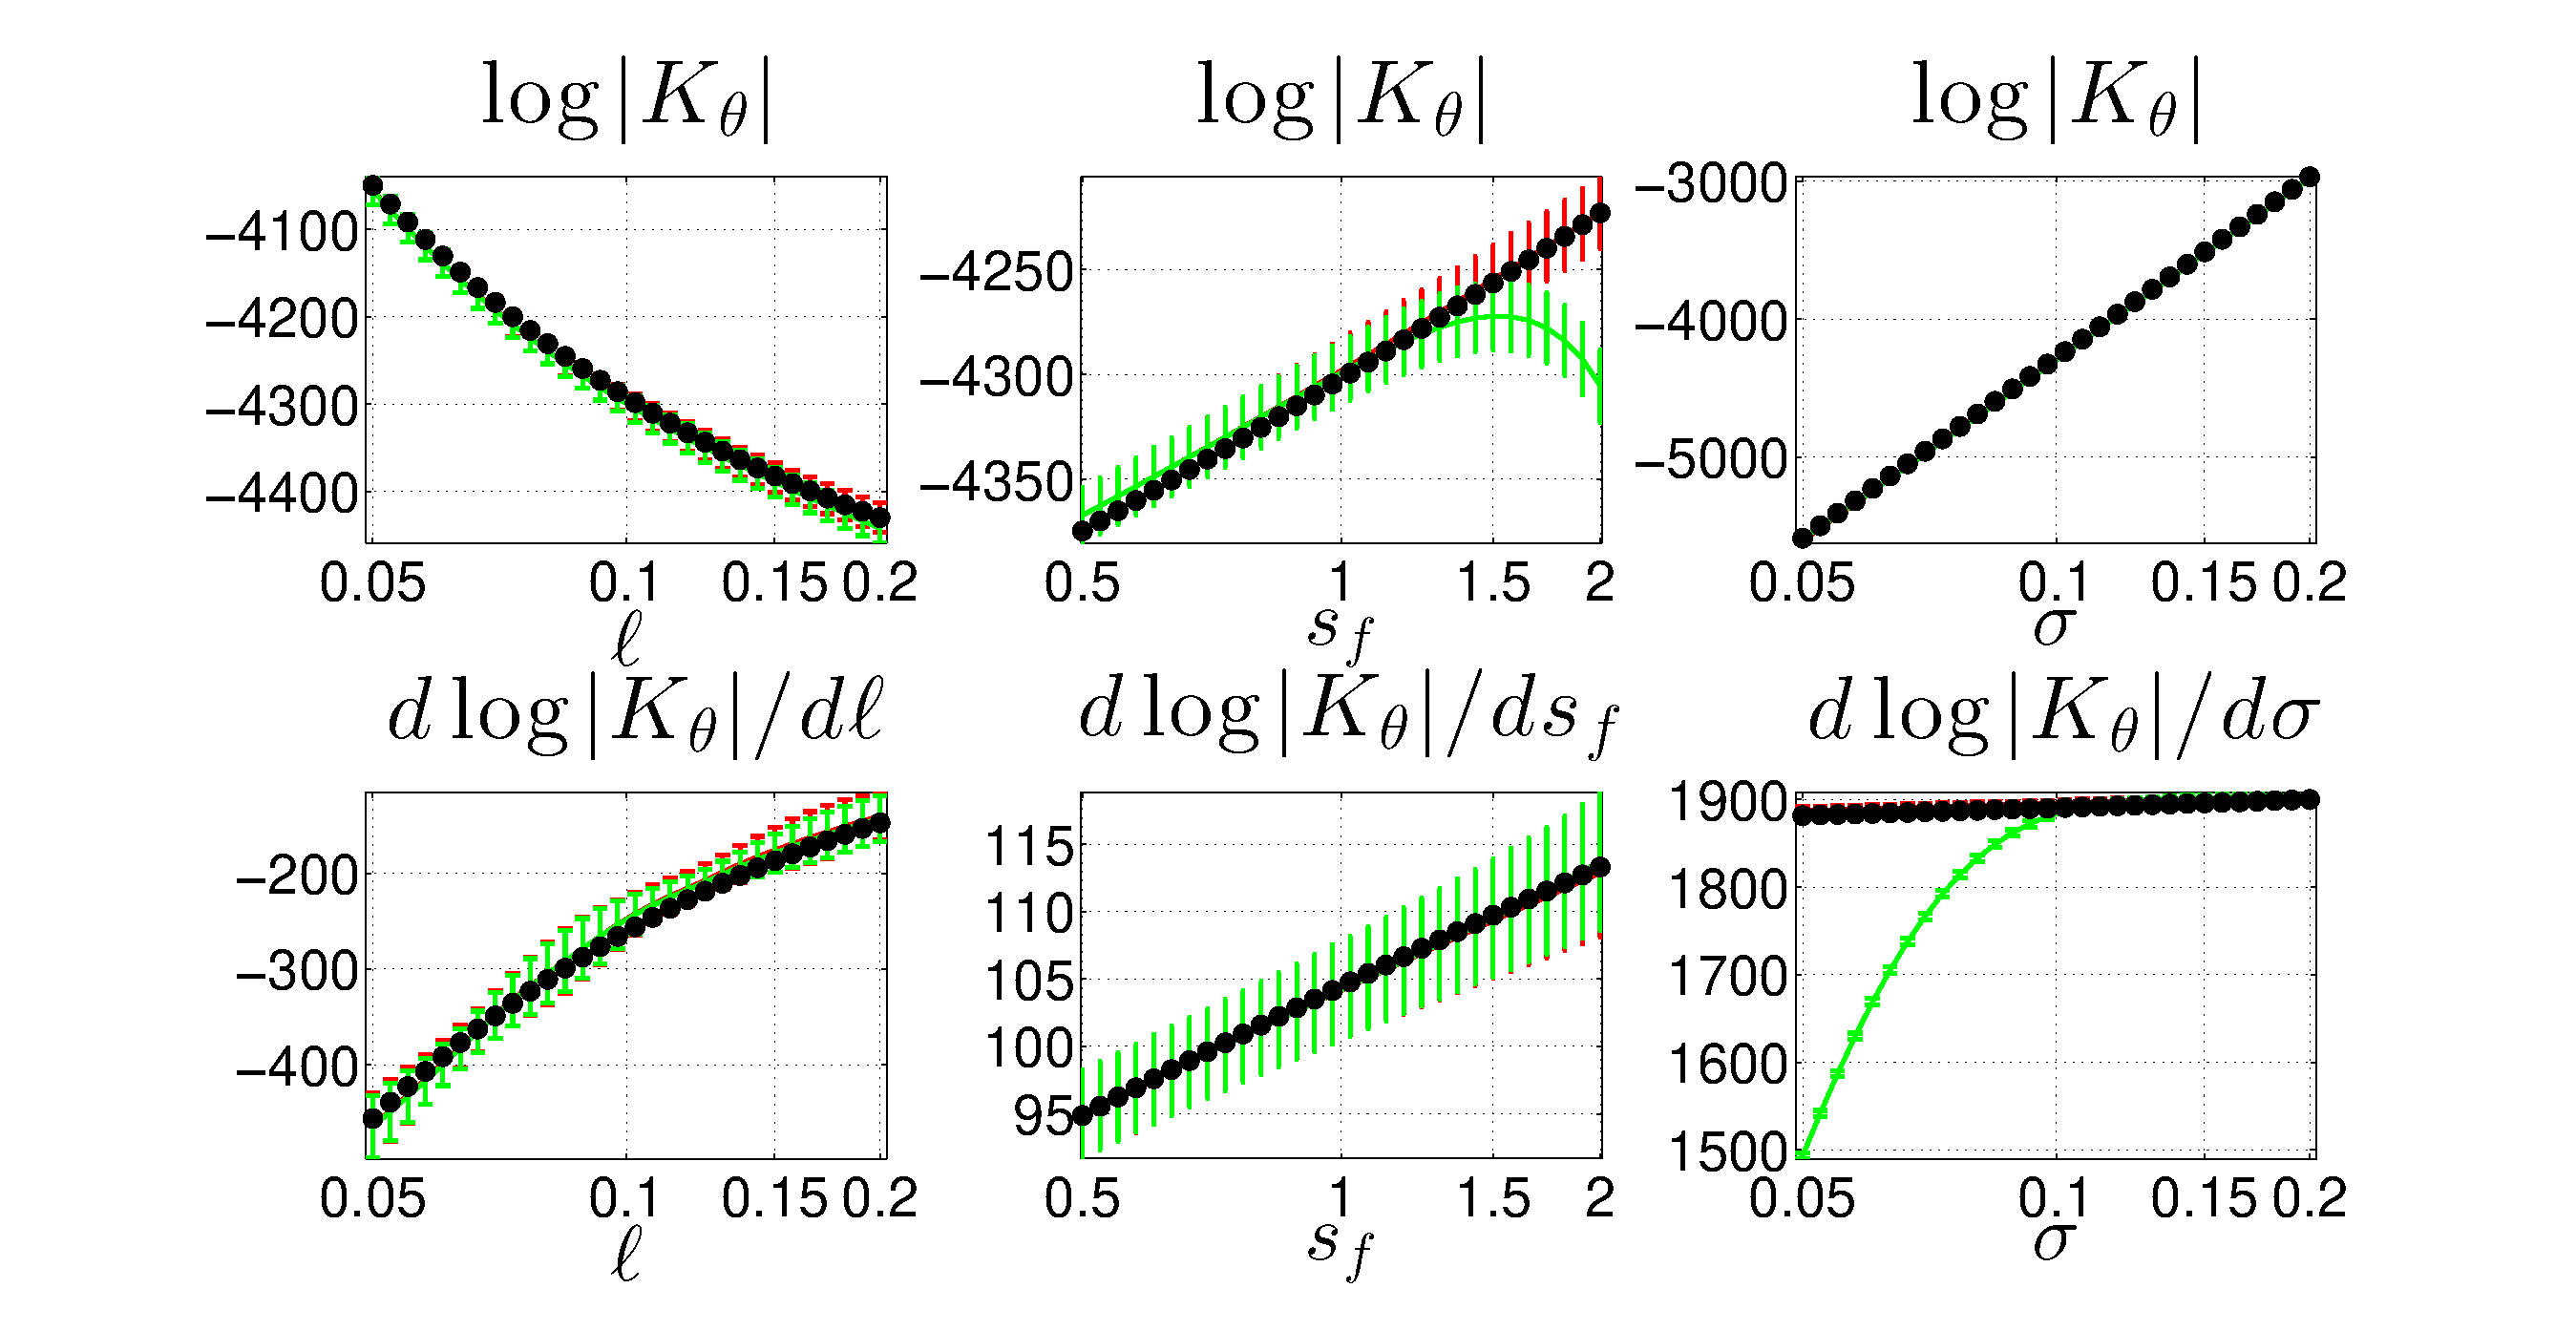
\includegraphics[width=\textwidth,trim=3.5cm 0cm 3.5cm 0cm,clip]
      {./sgp/pics/logdet_rbf}
      \caption{Log determinant for the RBF kernel}\label{fig:1dpert_c}
    \end{subfigure}
    \begin{subfigure}{0.46\textwidth}
      \centering
      \includegraphics[width=\textwidth,trim=3.5cm 0cm 3.5cm 0cm,clip]
      {./sgp/pics/logdet_Matern}
      \caption{Log determinant for the Mat\'ern kernel}\label{fig:1dpert_d}
    \end{subfigure}
    \caption{1\hyp{}dimensional perturbations for the exact RBF and 
    Mat\'ern\hyp{}1/2 kernel where the data is $1000$ equally spaced points in
    the interval $[0,4]$. The exact values are ($\bullet$), Lanczos is ({
    \color{red}-----}), Chebyshev is ({\color{green}-----}). The error bars of
    Lanczos and Chebyshev are $1$ standard deviation and were computed from $10$
    runs with different probe vectors}\label{fig:1dpert}
  \end{center}
\end{figure}

\begin{figure}[ht]
  \begin{center}
    \begin{subfigure}{0.46\textwidth}
      \centering
      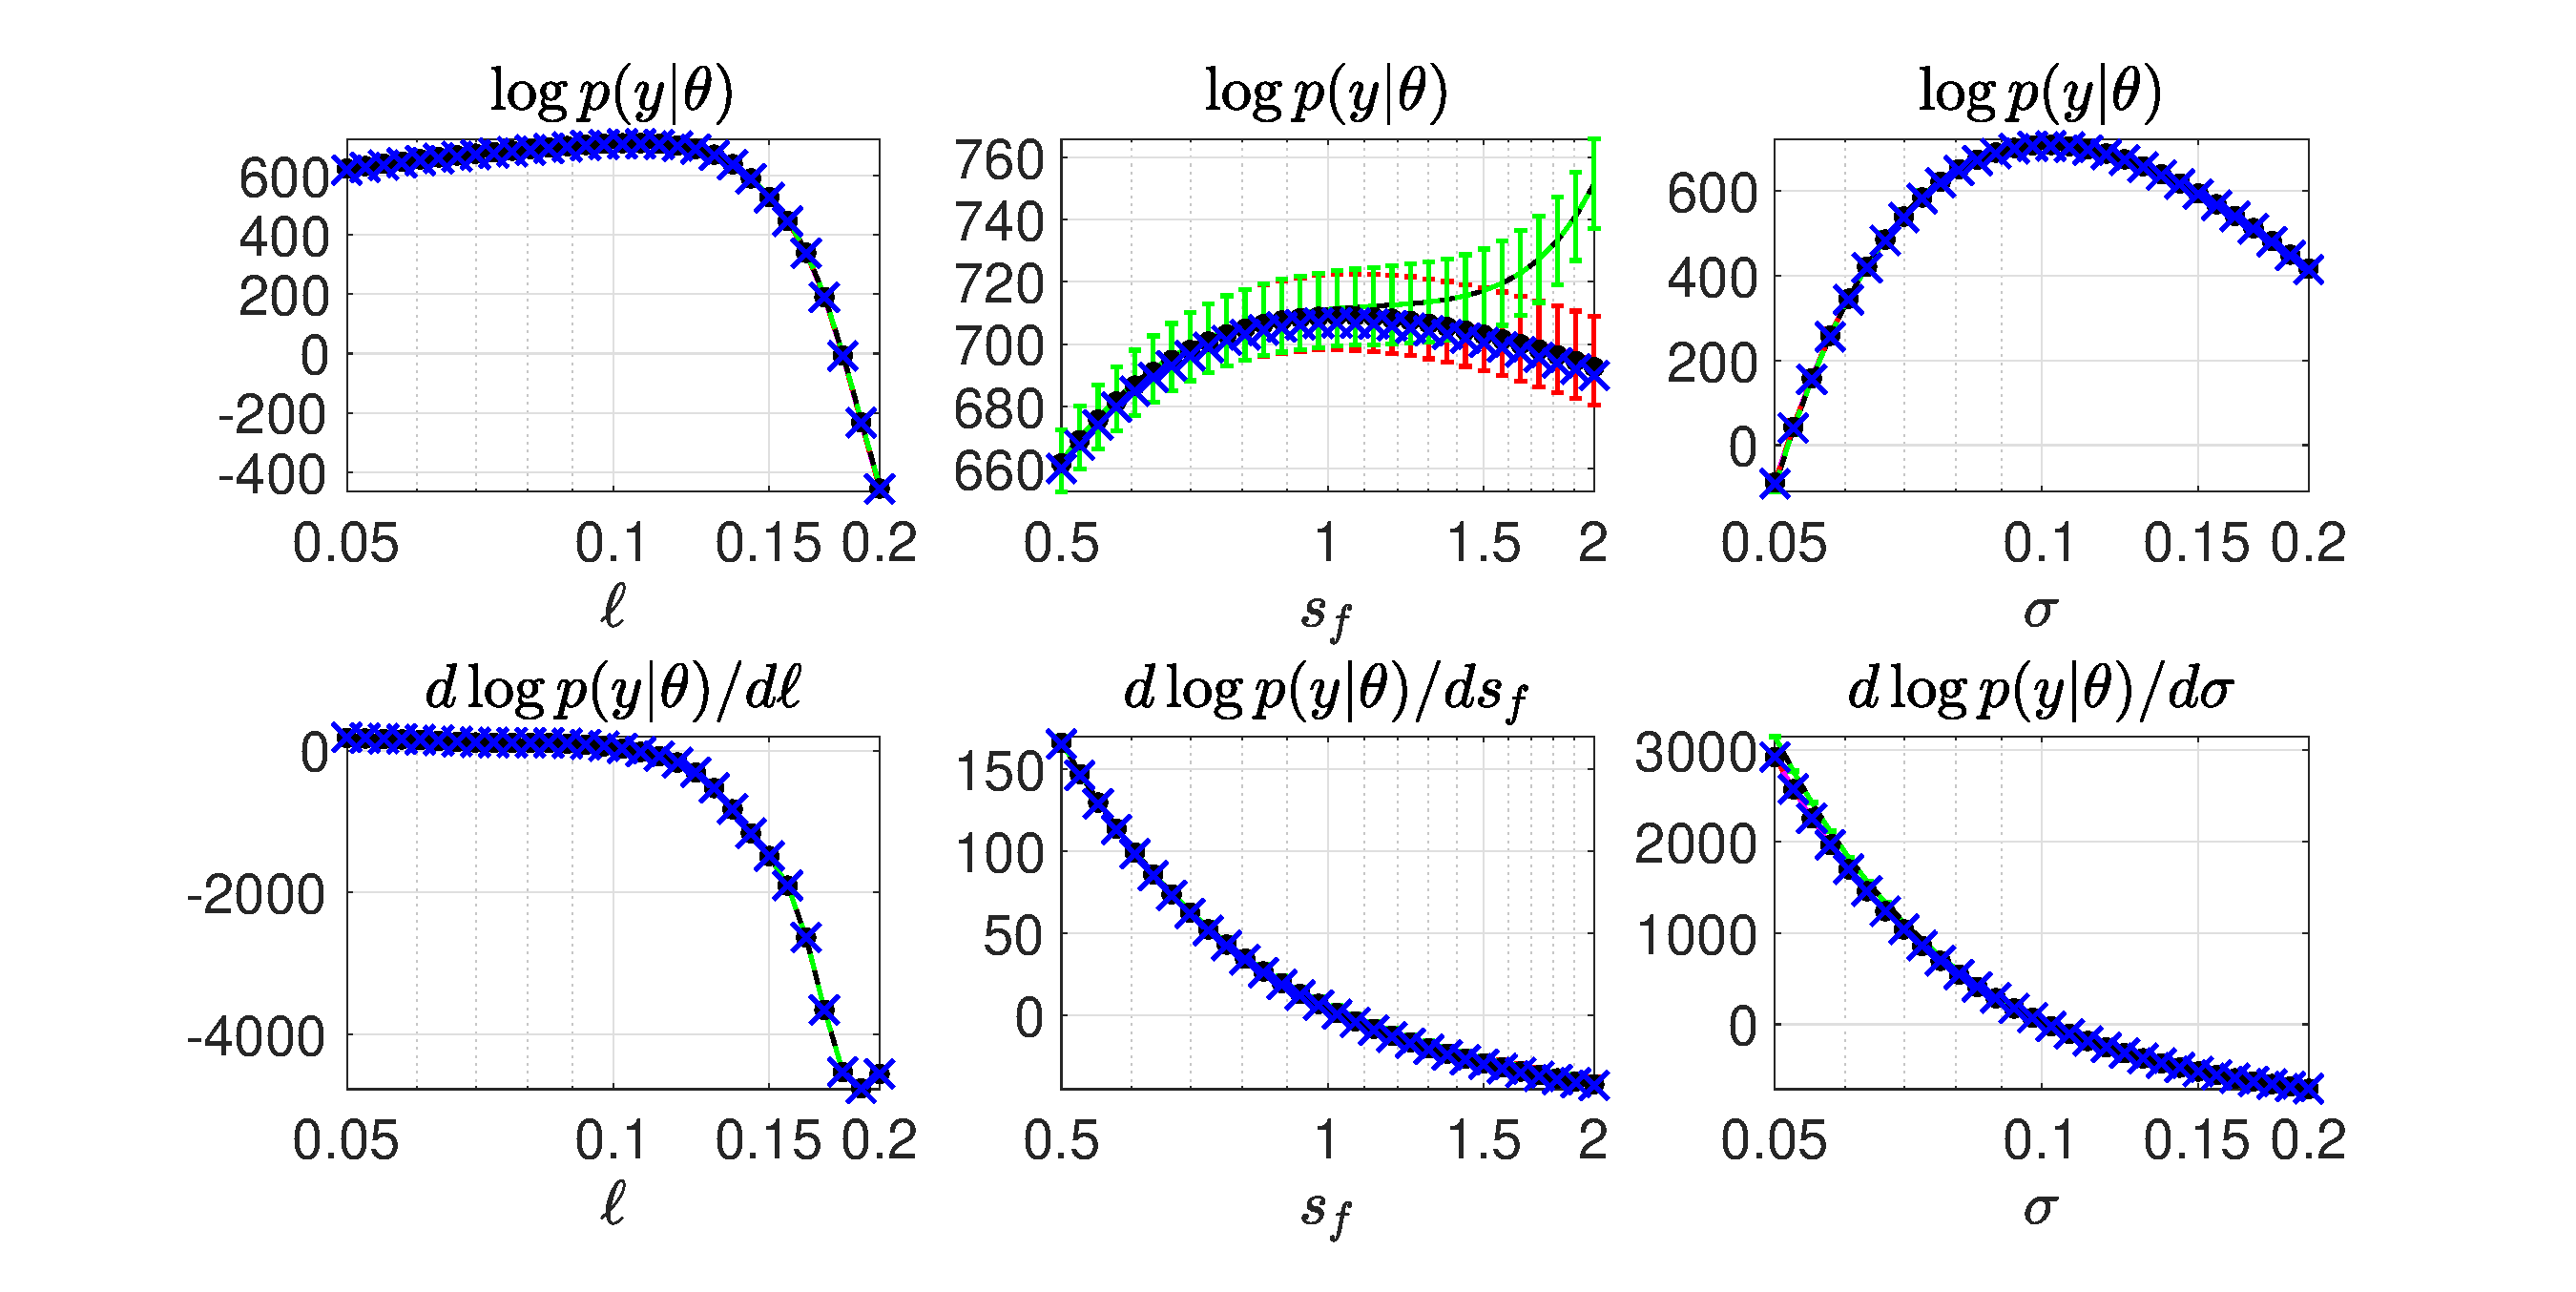
\includegraphics[width=\textwidth,trim=2.5cm 0cm 3.5cm 0cm,clip]
      {./sgp/pics/loglik_rbf_apx}
      \caption{Log marginal likelihood for the RBF \\kernel}
      \label{fig:1dpert_kissgp_a}
    \end{subfigure}
    \begin{subfigure}{0.46\textwidth}
      \centering
      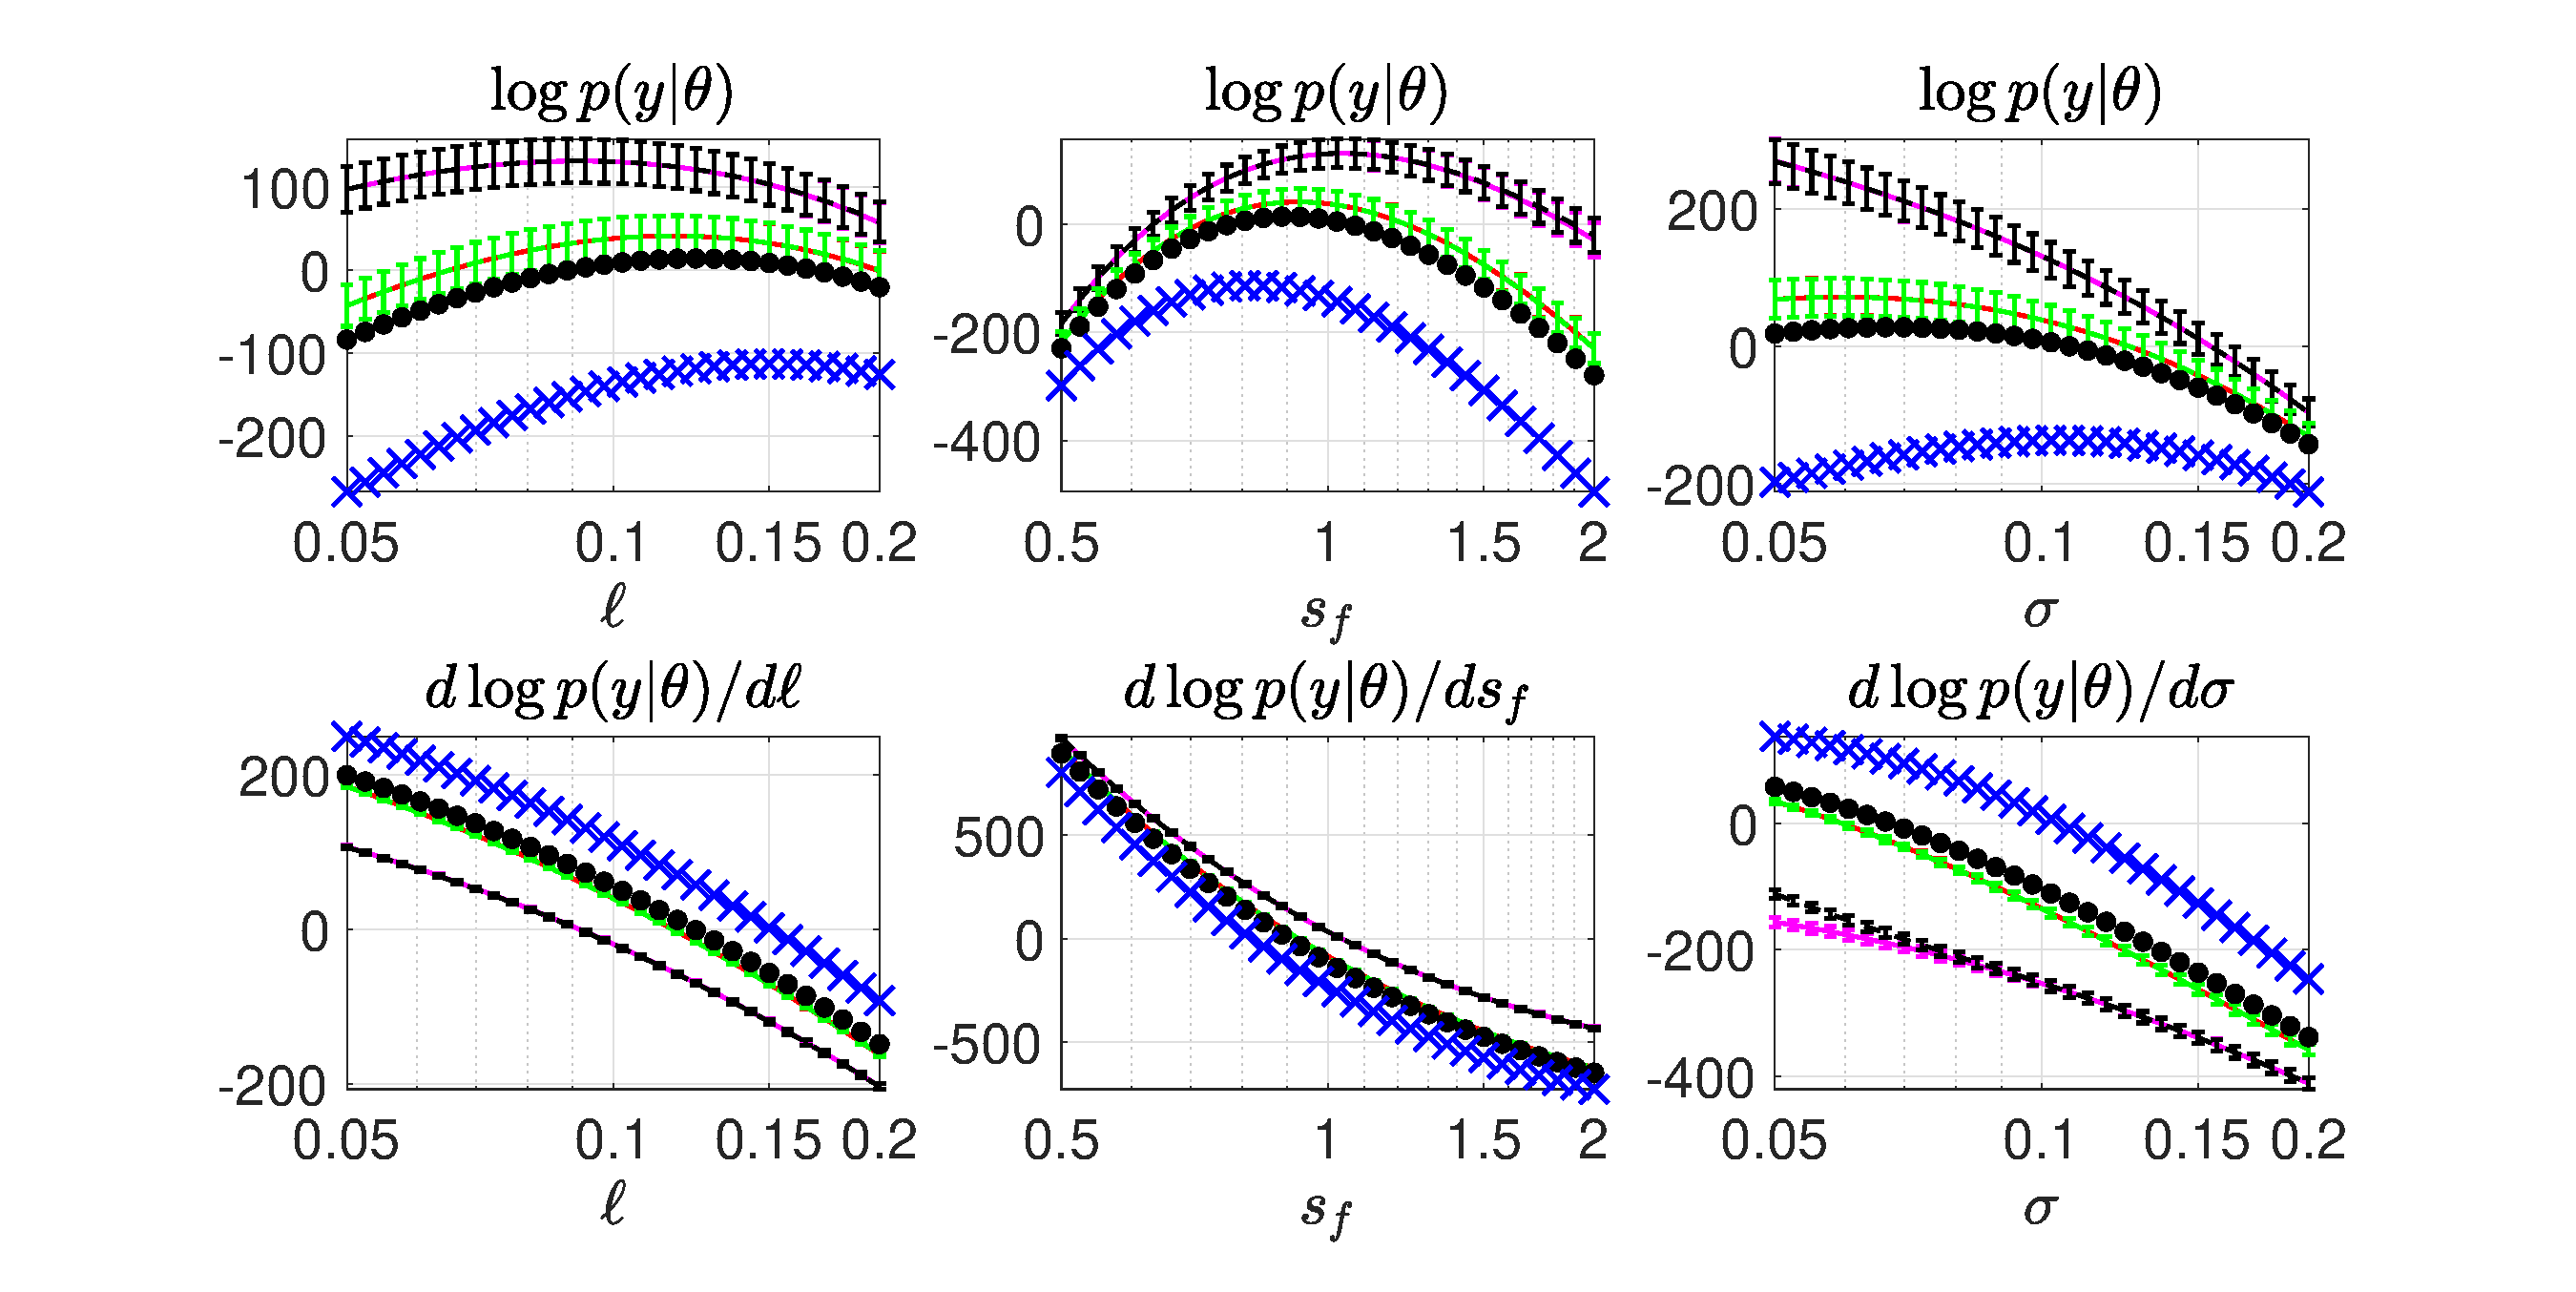
\includegraphics[width=\textwidth,trim=2.5cm 0cm 3.5cm 0cm,clip]
      {./sgp/pics/loglik_matern_apx}
      \caption{Log marginal likelihood for the Mat\'ern \\kernel}
      \label{fig:1dpert_kissgp_b}
    \end{subfigure}
    \begin{subfigure}{0.46\textwidth}
      \centering
      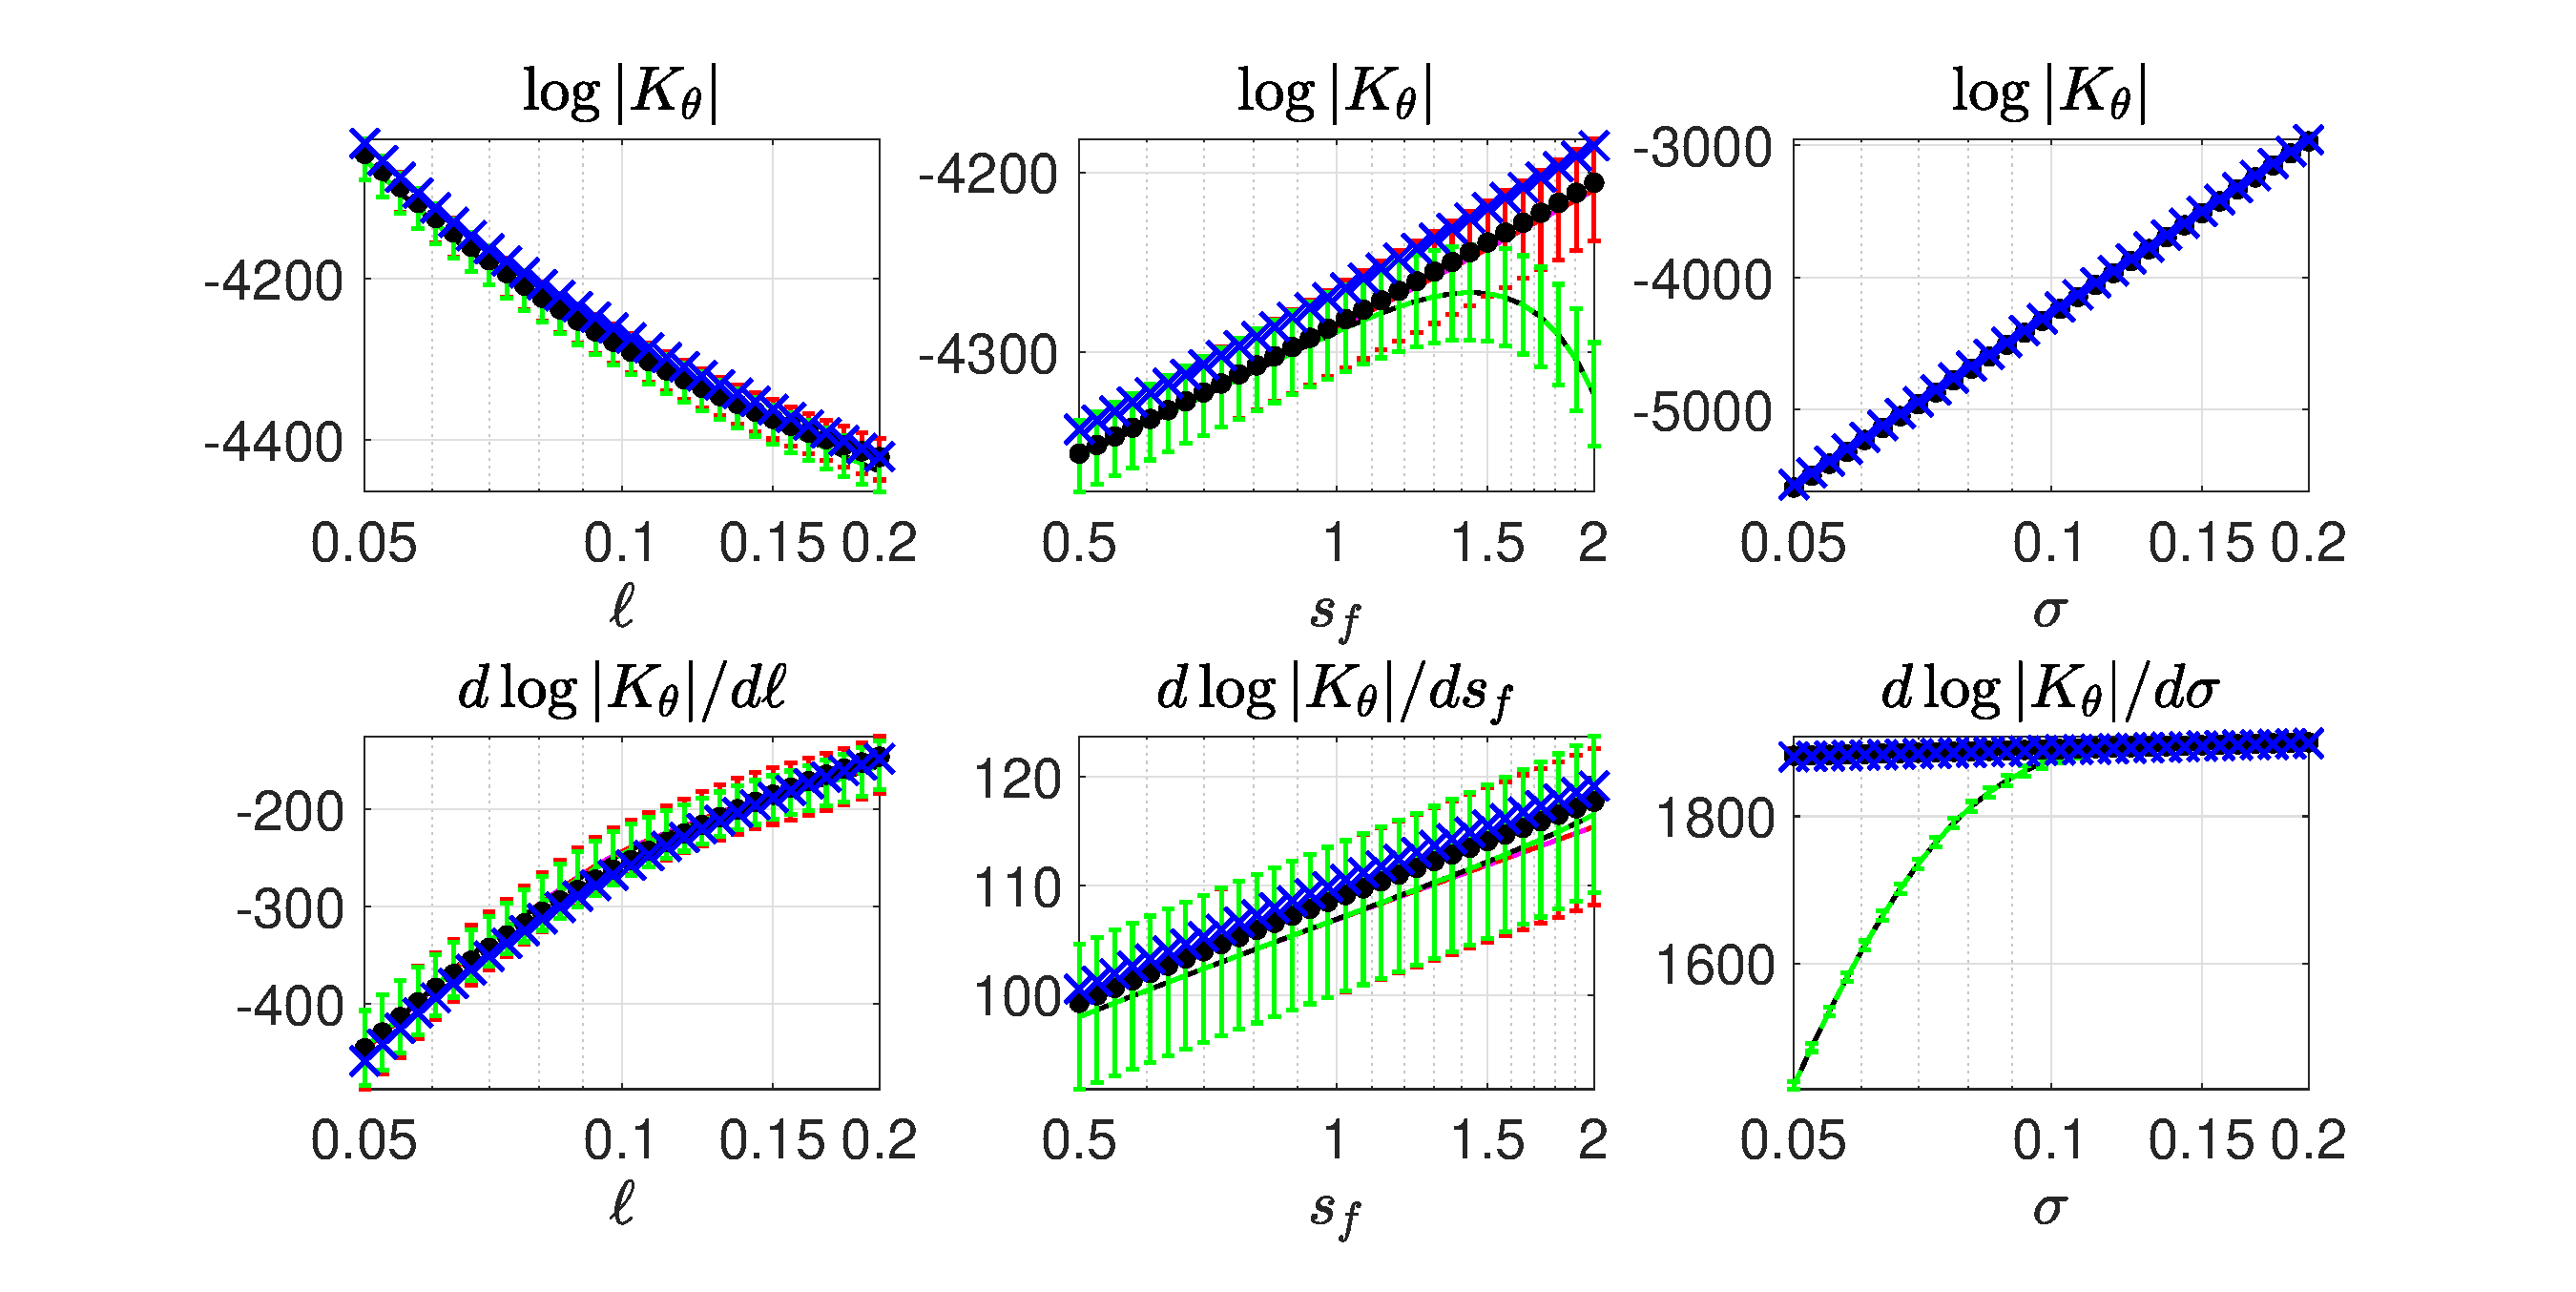
\includegraphics[width=\textwidth,trim=2.5cm 0cm 3.5cm 0cm,clip]
      {./sgp/pics/logdet_rbf_apx}
      \caption{Log determinant for the RBF kernel}
      \label{fig:1dpert_kissgp_c}
    \end{subfigure}
    \begin{subfigure}{0.46\textwidth}
      \centering
      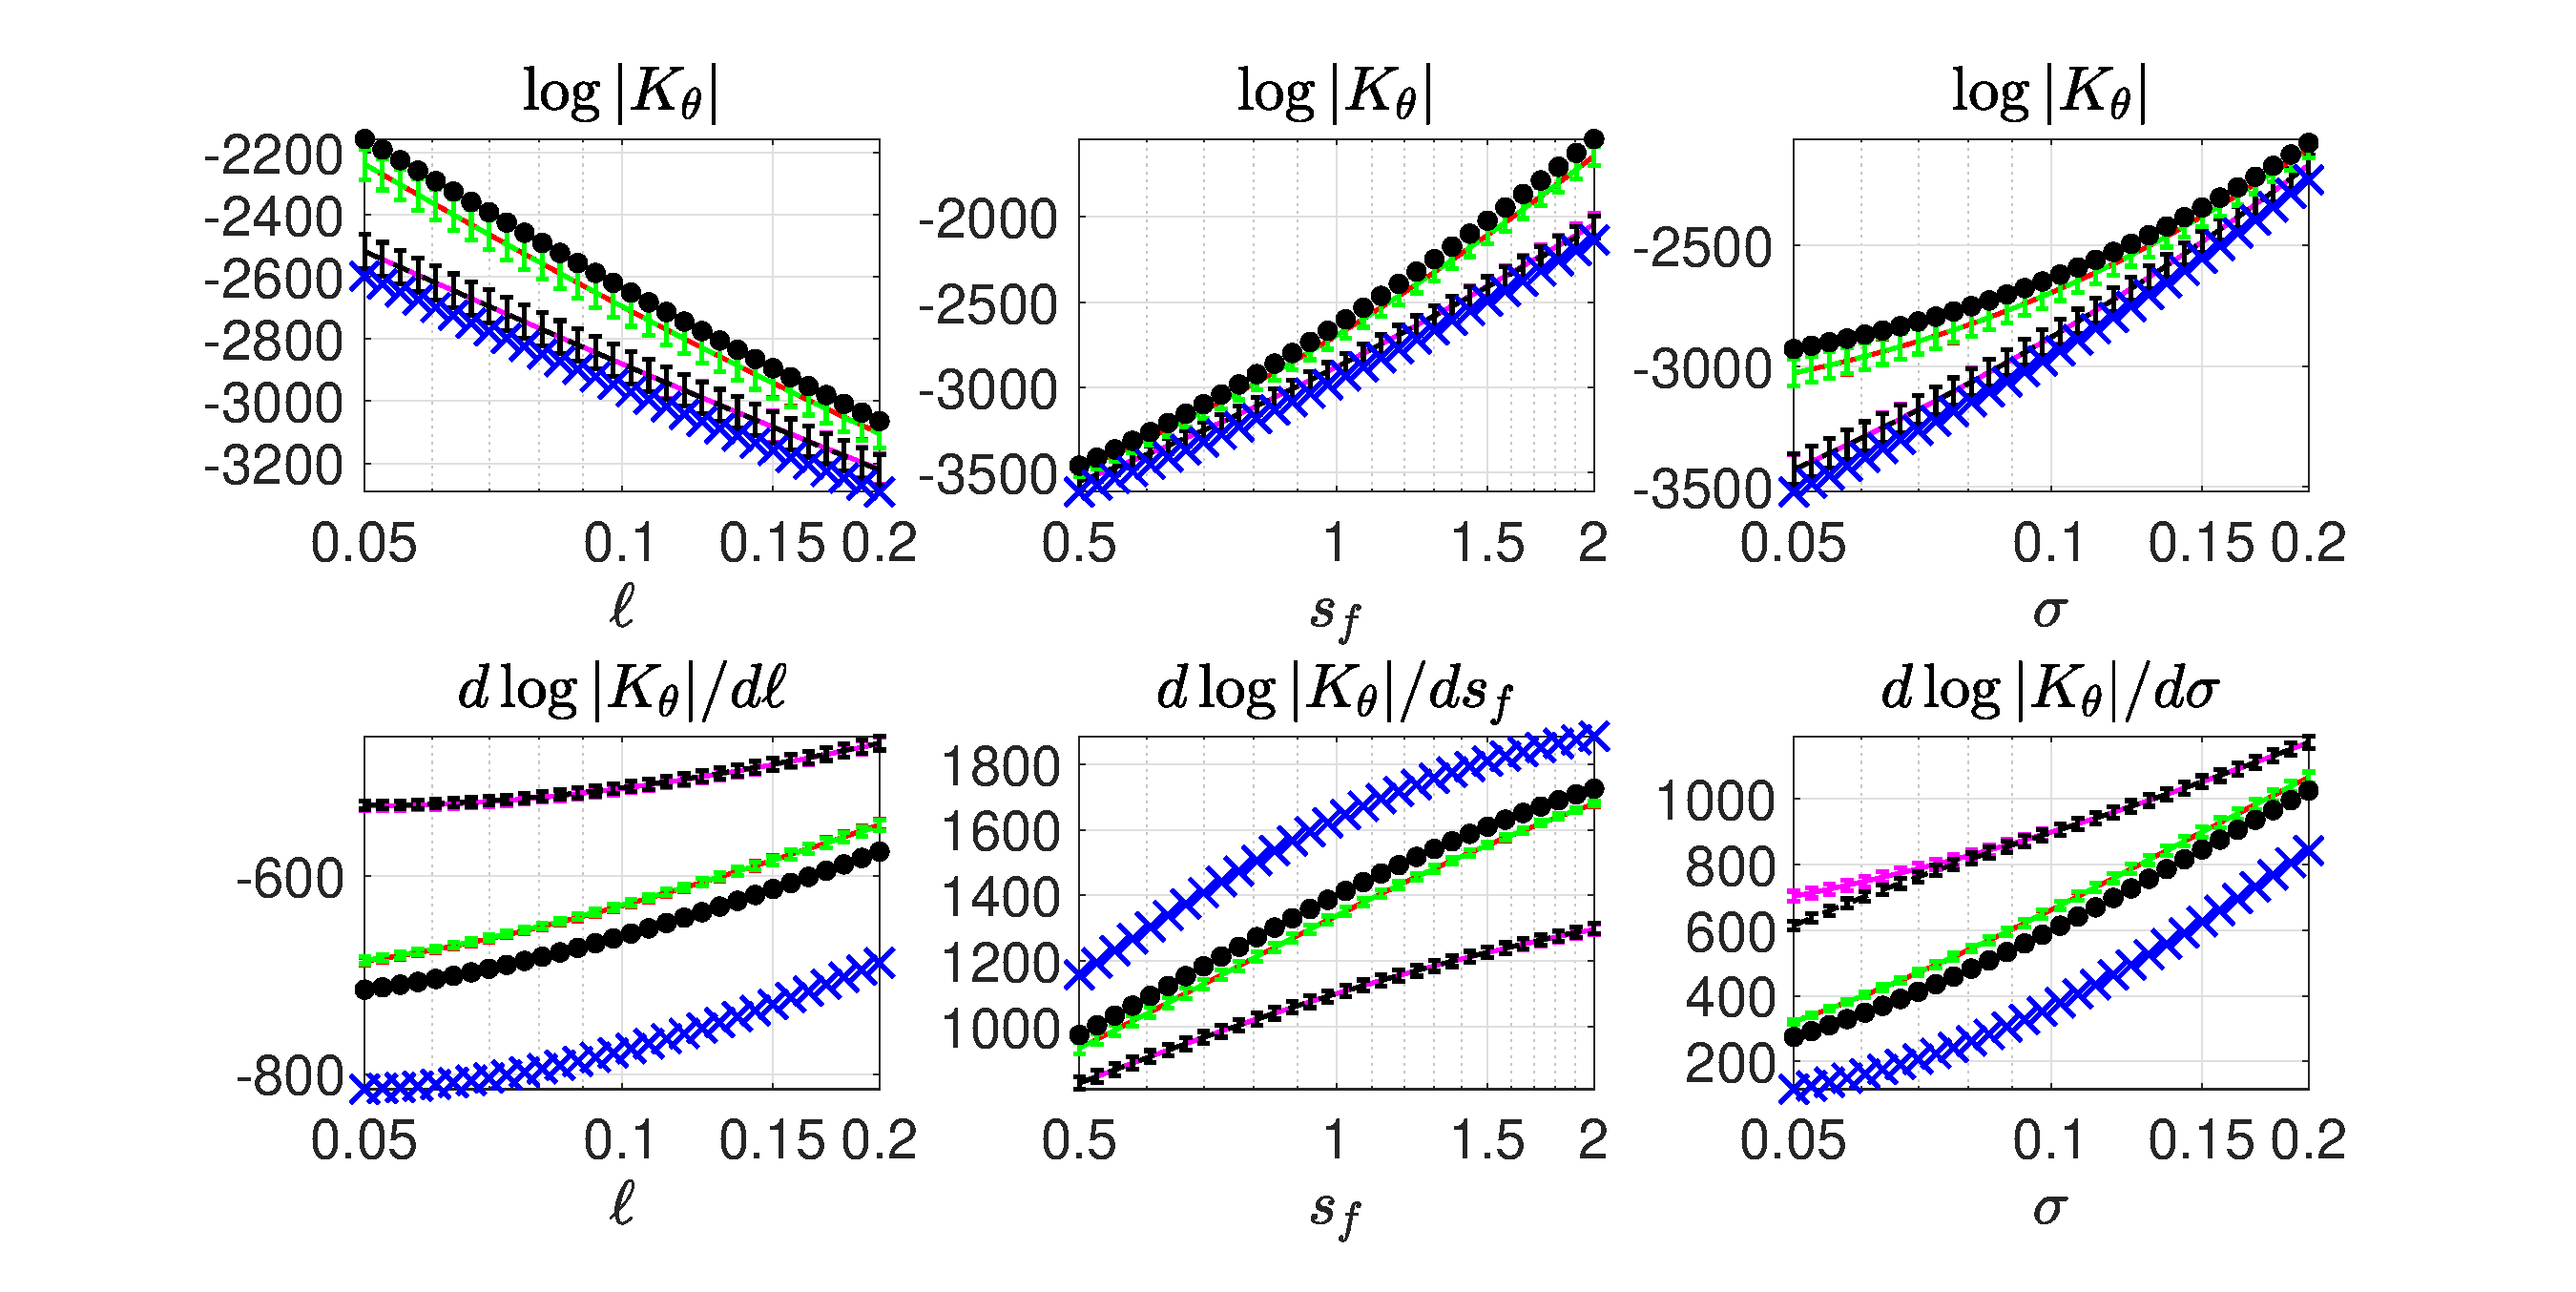
\includegraphics[width=\textwidth,trim=2.5cm 0cm 3.5cm 0cm,clip]
      {./sgp/pics/logdet_matern_apx}
      \caption{Log determinant for the Mat\'ern kernel}
      \label{fig:1dpert_kissgp_d}
    \end{subfigure}
    \caption{1\hyp{}dimensional perturbations with the SKI (cubic)
    approximations of the RBF and Mat\'ern\hyp{}1/2 kernel where the data is
    1000 points drawn from $\calN(0,2)$. The exact values are ($\bullet$),
    Lanczos with diagonal replacement is ({\color{red}-----}), Chebyshev with
    diagonal replacement is ({\color{green}-----}), Lanczos without diagonal
    replacement is ({\color{magenta}-----}), Chebyshev without diagonal
    replacement is ({\color{black}-----}), and scaled eigenvalues is ({
    \color{blue} $\times$}). Diagonal replacement makes no perceptual difference
    for the RBF kernel so the lines are overlapping in this case. The error bars
    of Lanczos and Chebyshev are $1$ standard deviation and were computed from
    $10$ runs with different probe vectors}\label{fig:1dpert_kissgp}
 \end{center}
\end{figure}

Lanczos yields an excellent approximation to the log determinant and its
derivatives for both the exact and the approximate kernels, while Chebyshev
struggles with large values of $s_f$ and small values of $\sigma$ on the
exact and approximate RBF kernel. This is expected since Chebyshev has issues
with the singularity at zero while Lanczos has large quadrature weights
close to zero to compensate for this singularity. The scaled eigenvalue method
has issues with the approximate Mat\'ern\hyp{}1/2 kernel.

\subsection{Why Lanczos is Better Than Chebyshev}\label{sup:lanczoscheb}

In this experiment, we study the performance advantage of Lanczos over
Chebyshev. \cref{fig:spectrum} shows that the Ritz values of Lanczos quickly
converge to the spectrum of the RBF kernel thanks to the absence of interior
eigenvalues. The Chebyshev approximation shows the expected equioscillation
behavior. More importantly, the Chebyshev approximation for logarithms has its
greatest error near zero where the majority of the eigenvalues are, and those
also have the heaviest weight in the log determinant.

Another advantage of Lanczos is that it requires minimal knowledge of the
spectrum, while Chebyshev needs the extremal eigenvalues for rescaling. In
addition, with Lanczos we can get the derivatives with only one MVM per 
hyper\hyp{}parameter, while Chebyshev requires an MVM at each iteration, leading
to extra computation and memory usage.

\begin{figure}[ht]
  \begin{center}
    \begin{subfigure}{0.46\textwidth}
      \centering
      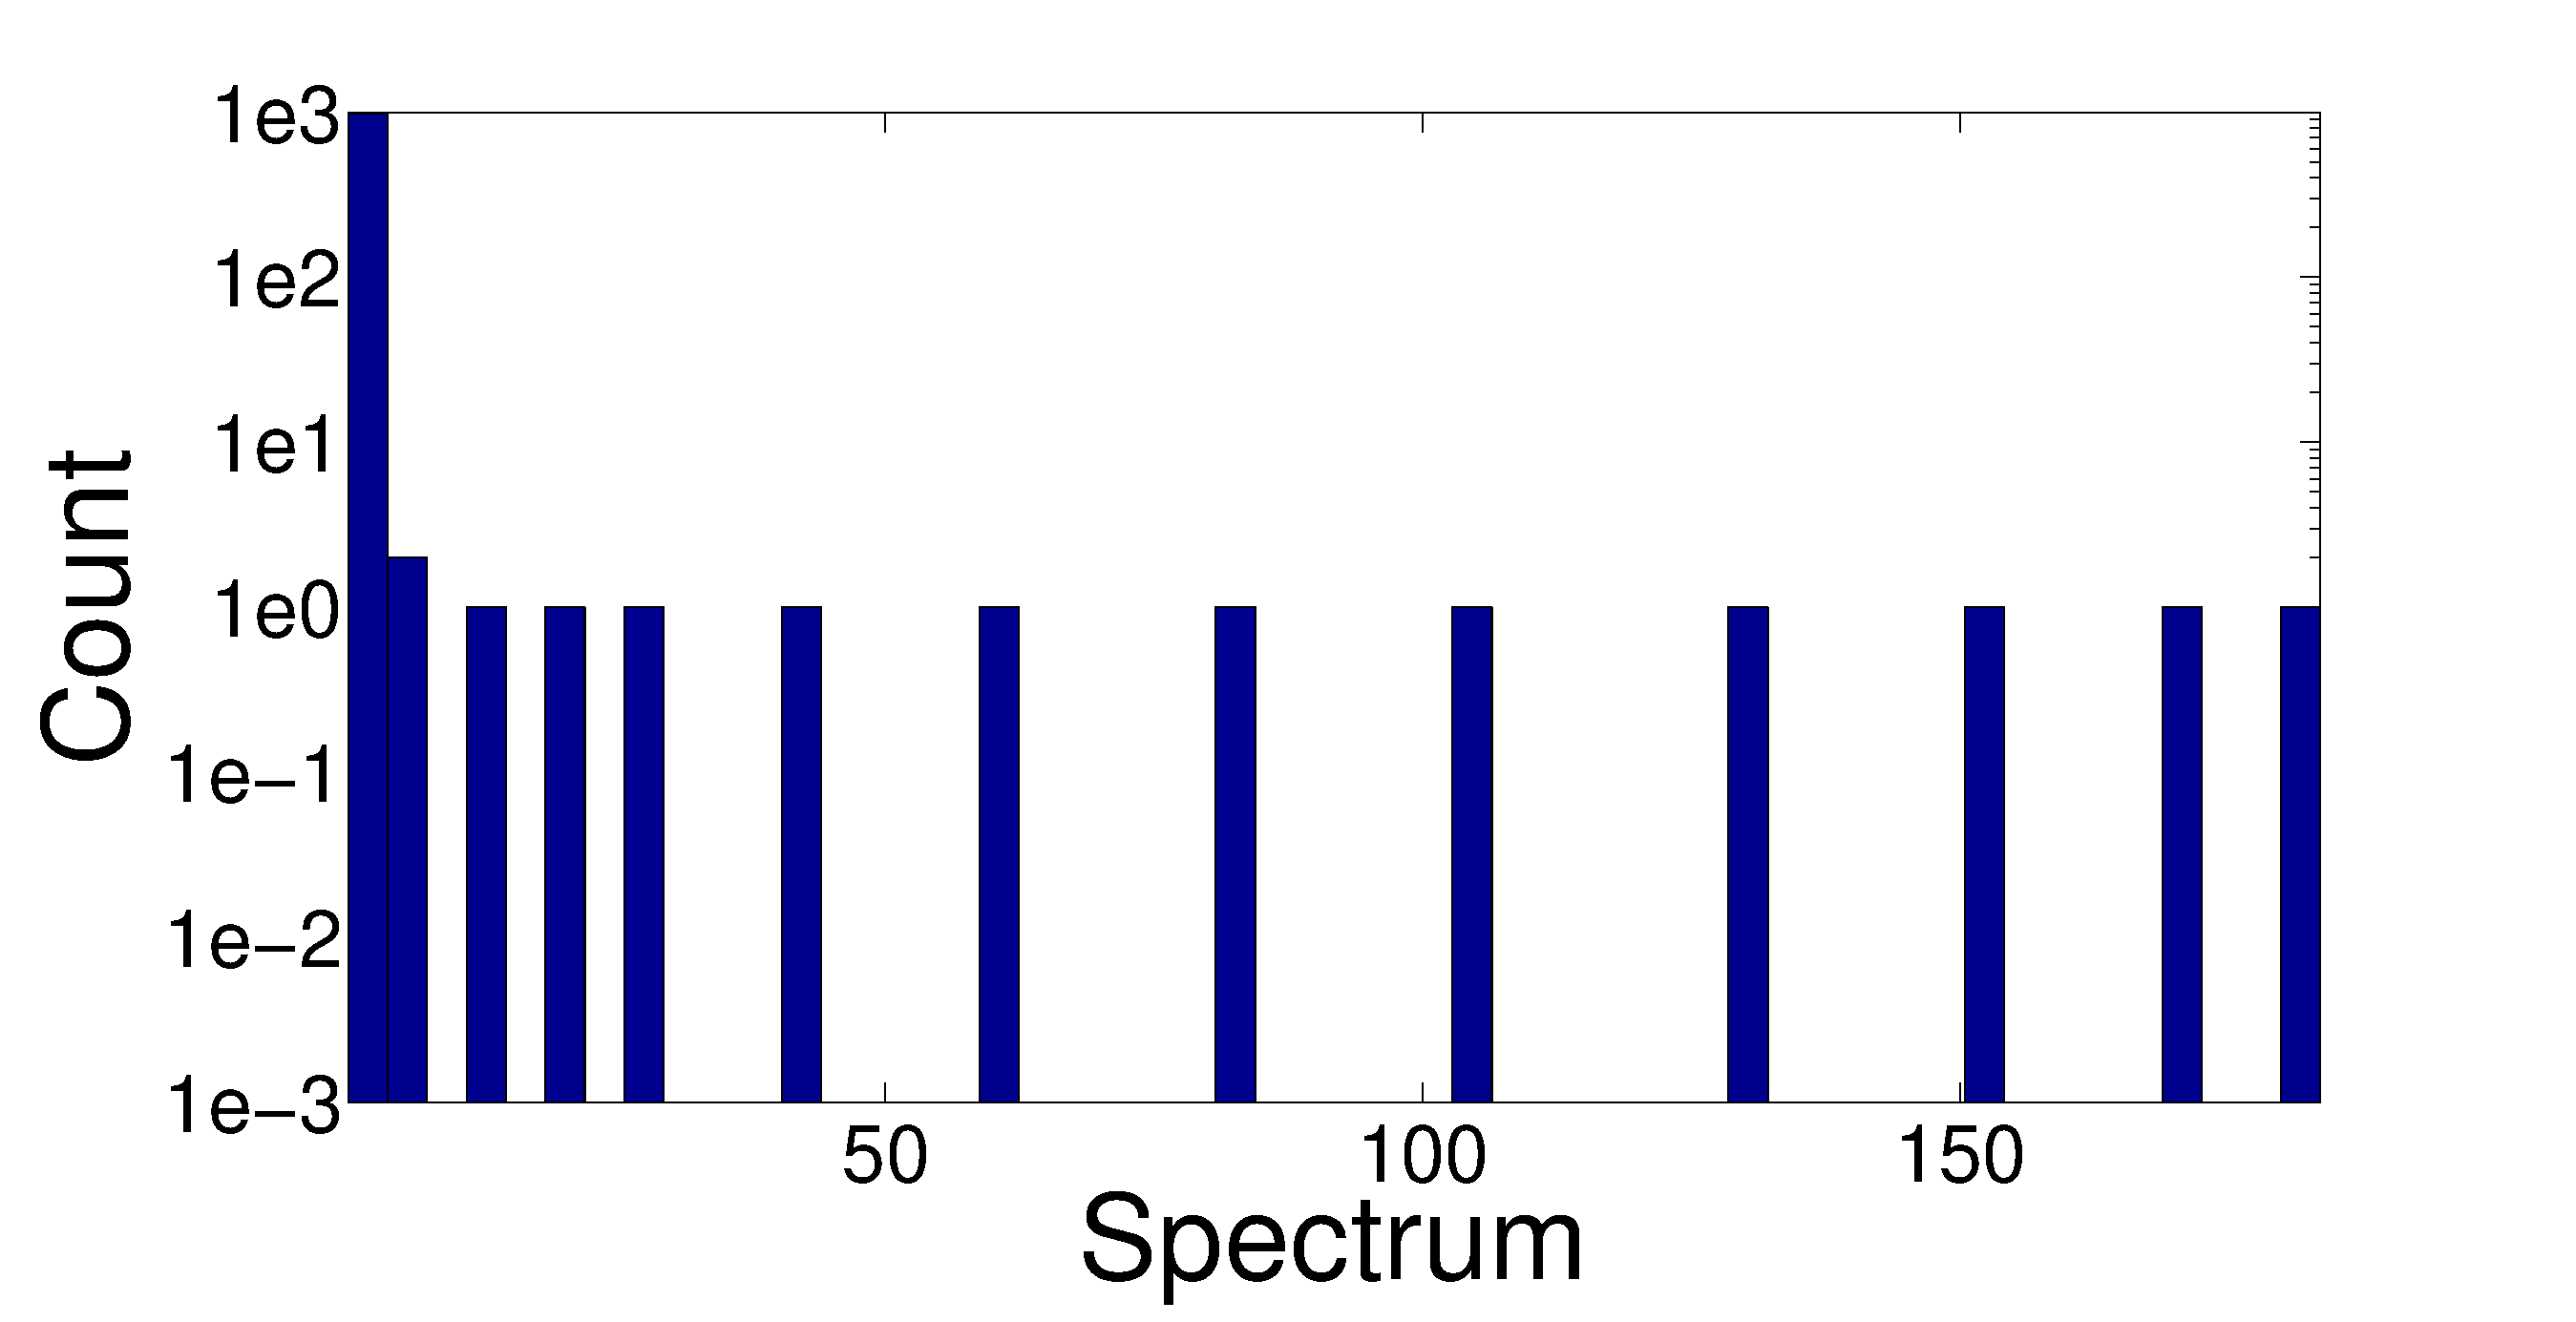
\includegraphics[width=\textwidth,trim=0cm 0cm 2.5cm 0.5cm,clip]
      {./sgp/pics/true_spectral}
      \caption{True spectrum}
      \label{fig:true_spectral}
    \end{subfigure}
    \begin{subfigure}{0.46\textwidth}
      \centering
      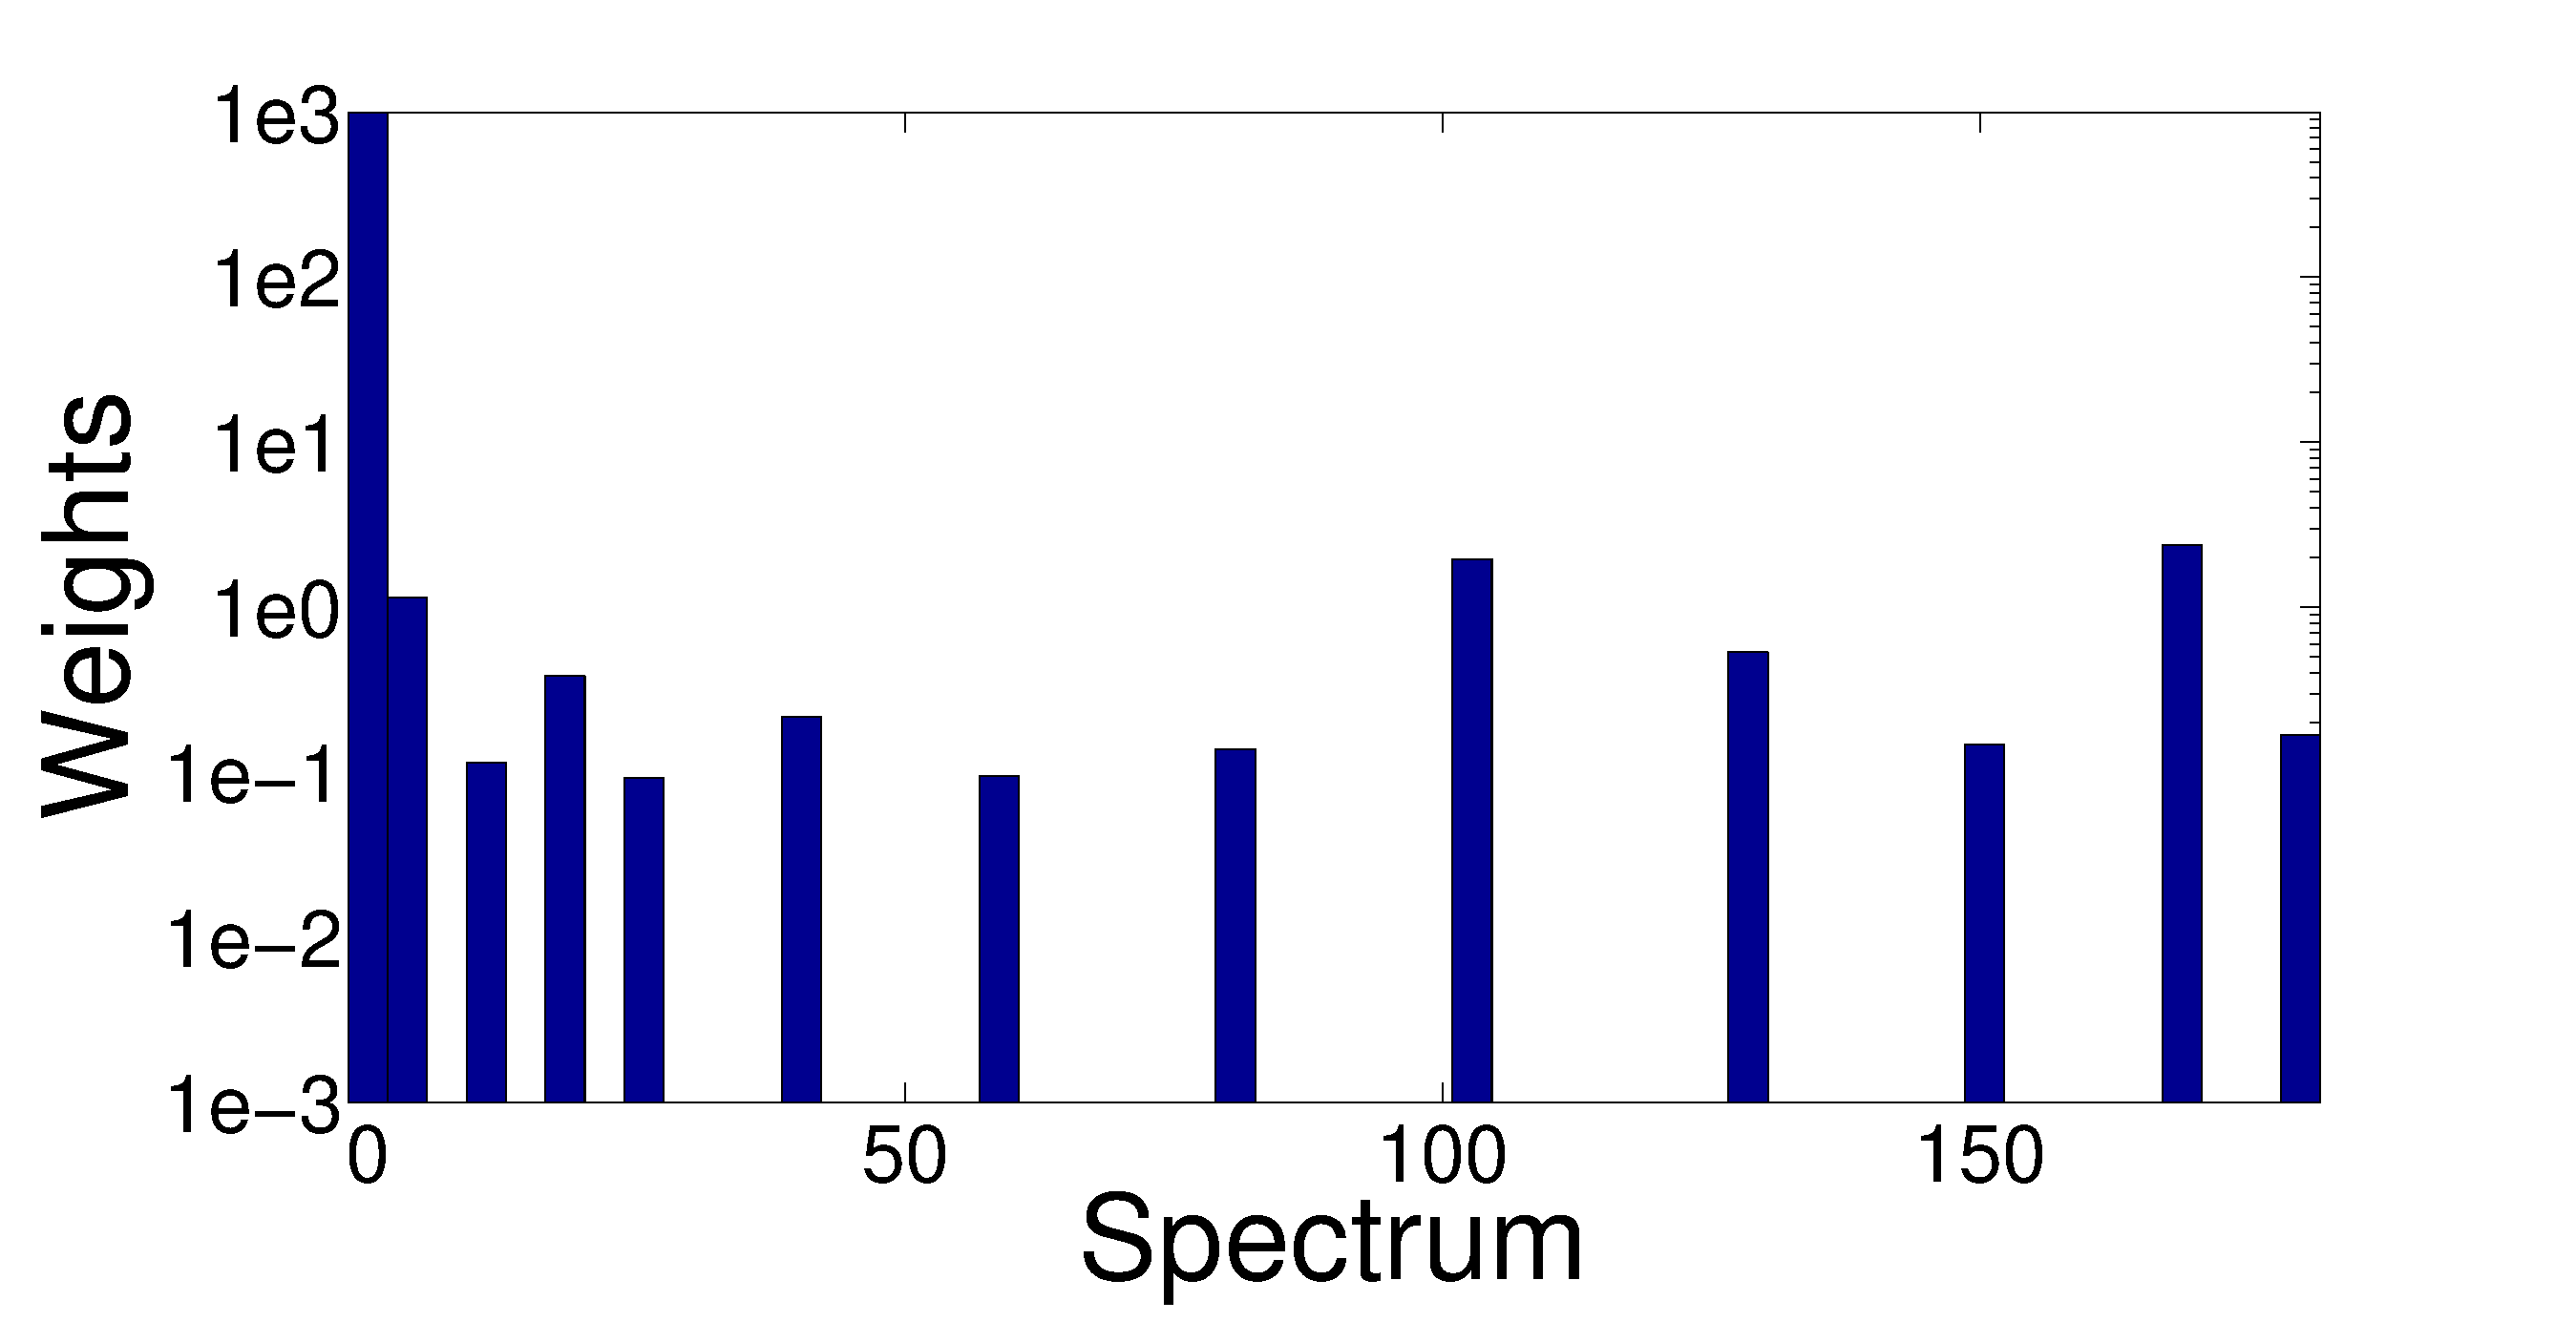
\includegraphics[width=\textwidth,trim=0cm 0cm 2.5cm 0.5cm,clip]
      {./sgp/pics/lanc_spectral}
      \caption{Lanczos weights}
      \label{fig:lanc_spectral}
    \end{subfigure}
    \begin{subfigure}{0.46\textwidth}
      \centering
      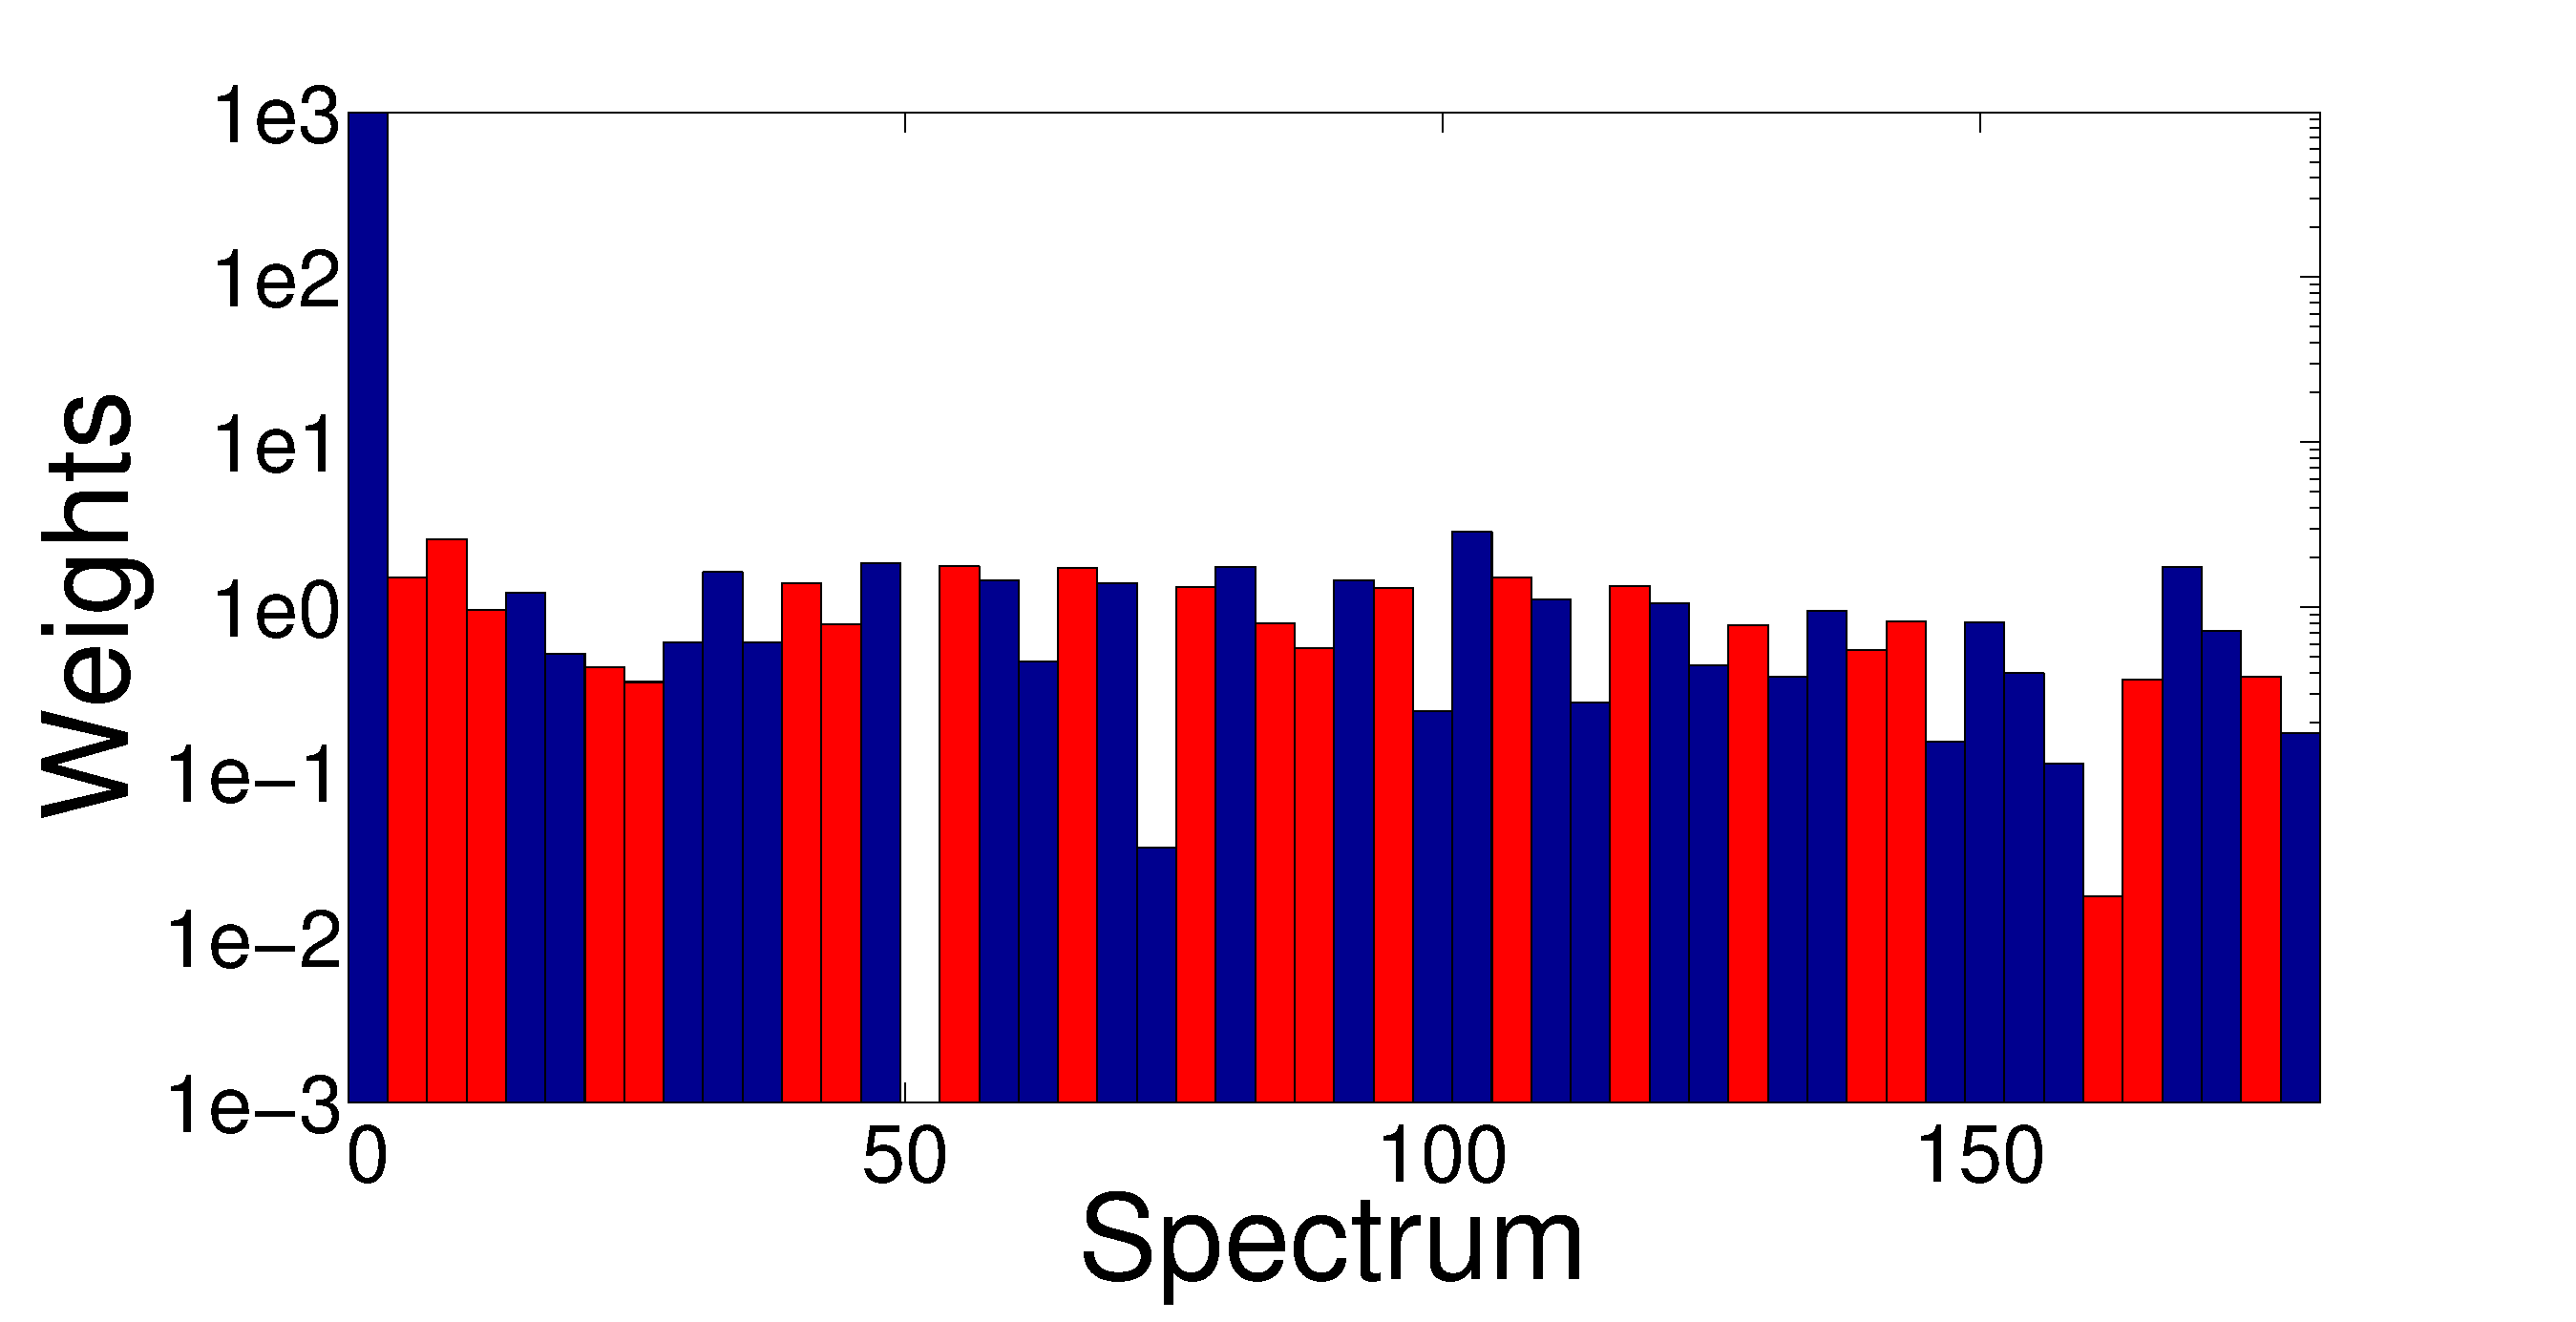
\includegraphics[width=\textwidth,trim=0cm 0cm 2.5cm 0.5cm,clip]
      {./sgp/pics/cheb_spectral}
      \caption{Chebyshev weights}
      \label{fig:cheb_spectral}
    \end{subfigure}
    \begin{subfigure}{0.46\textwidth}
      \centering
      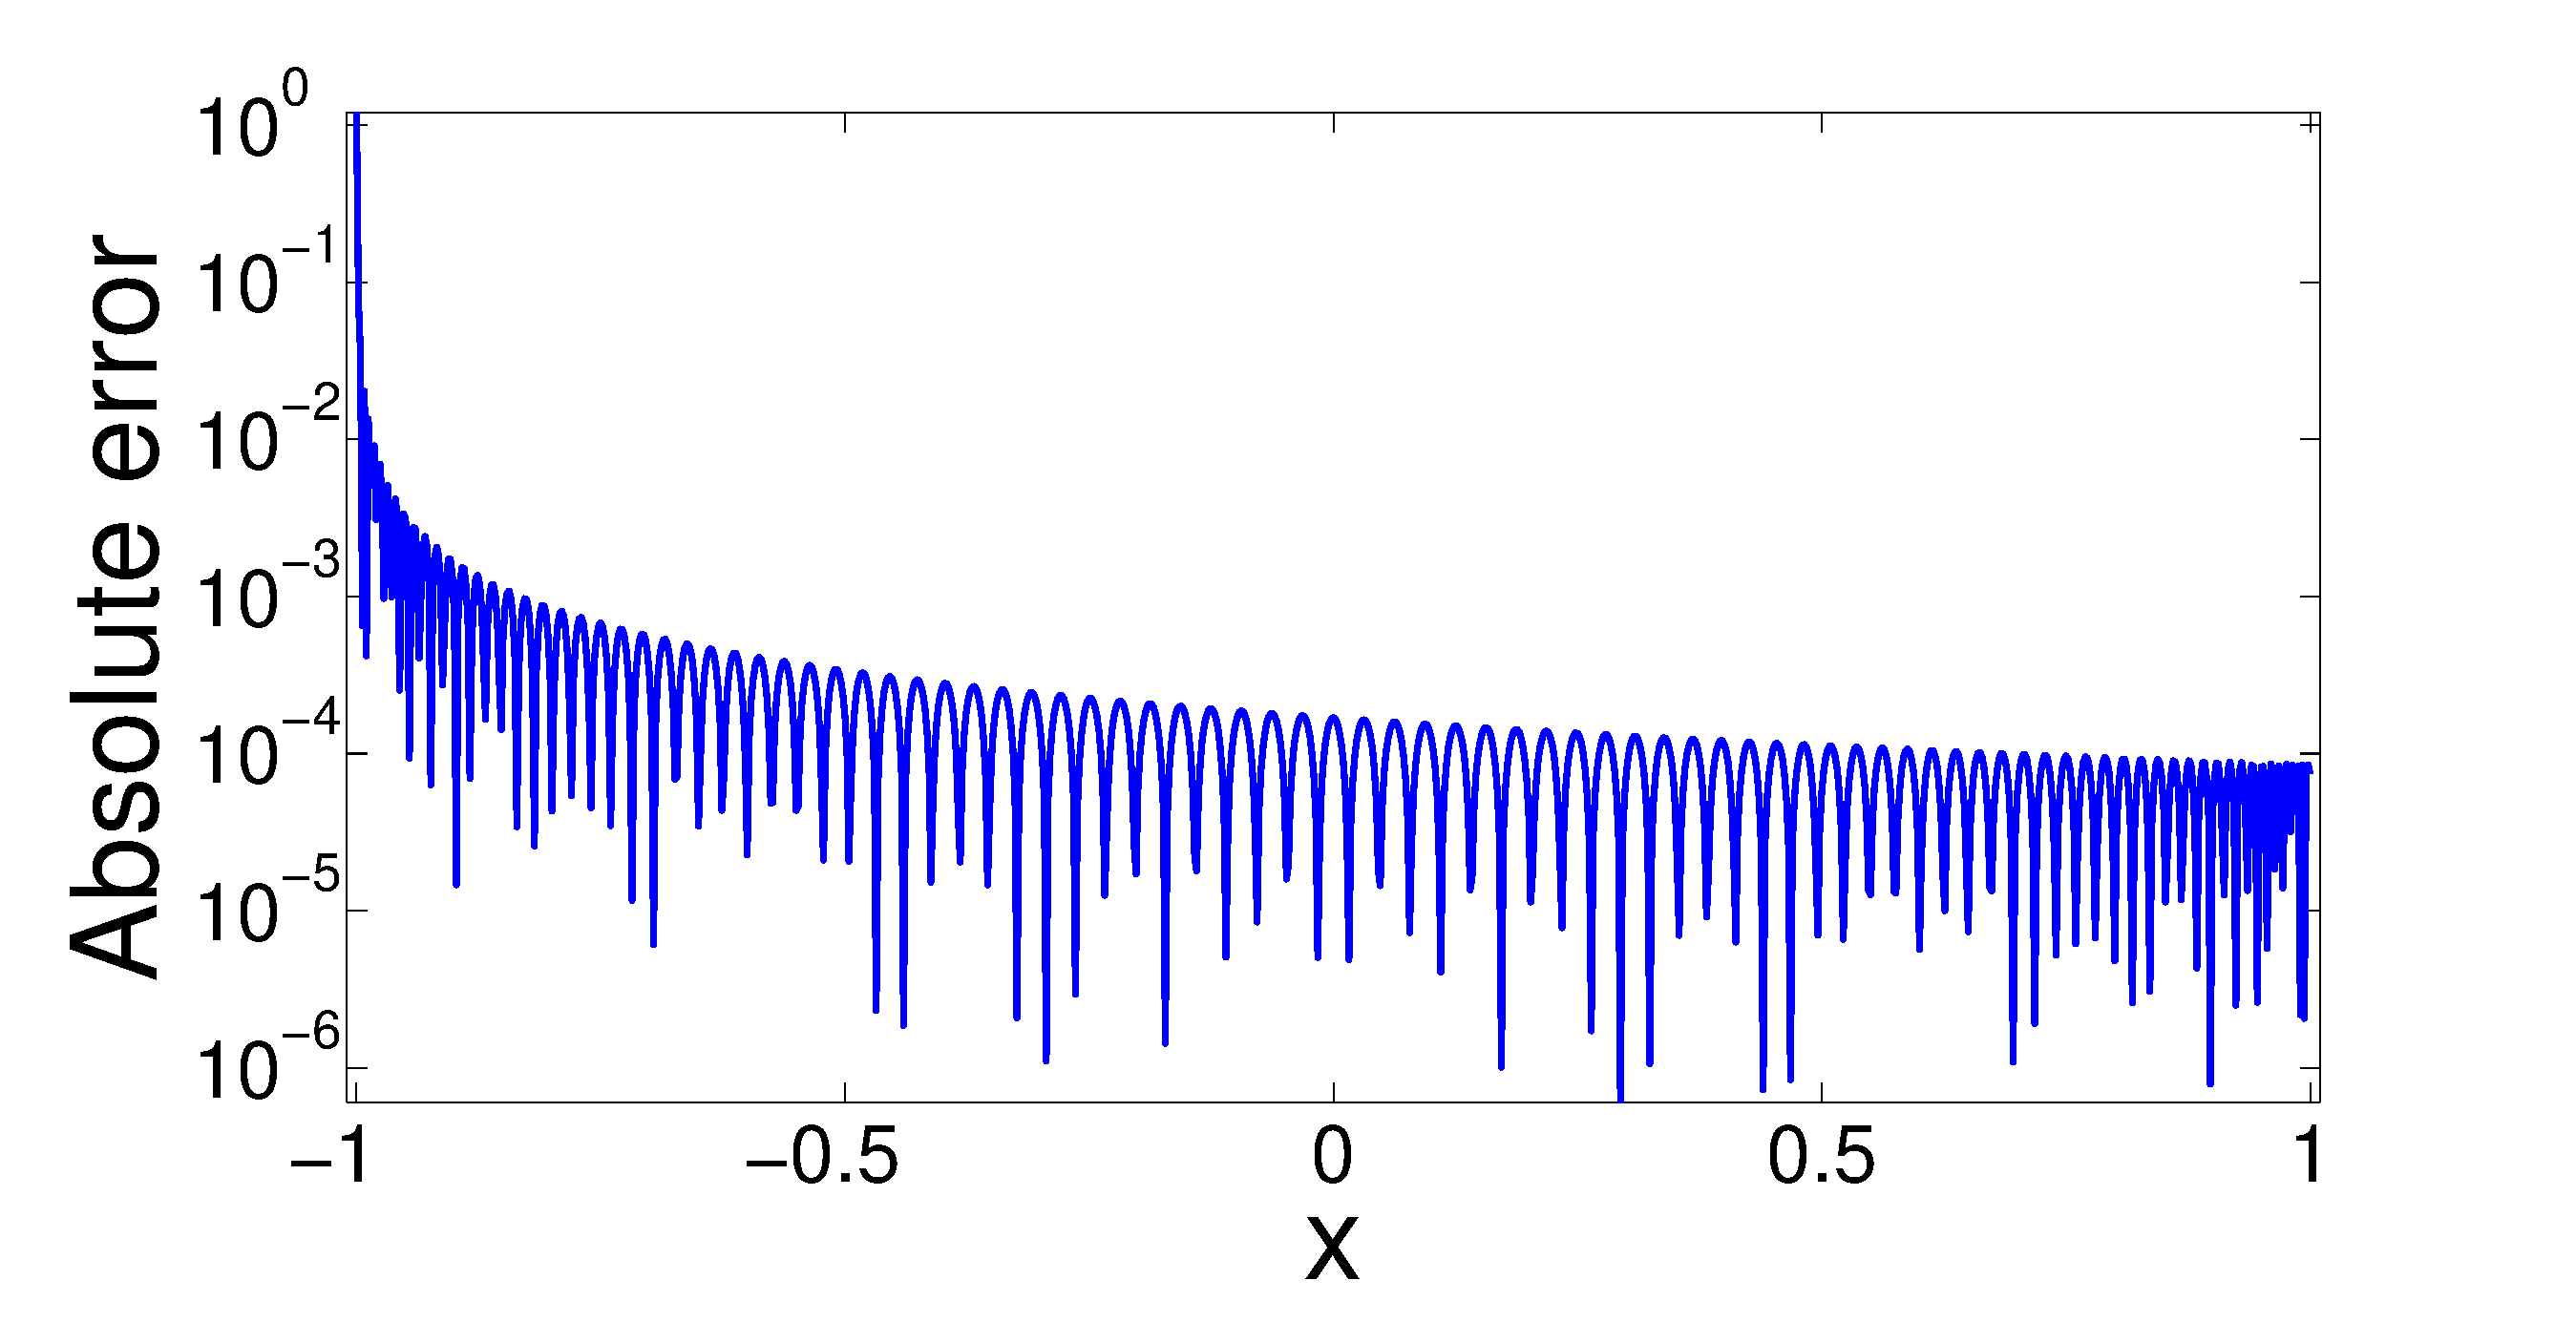
\includegraphics[width=\textwidth,trim=0cm 0cm 2.5cm 0.5cm,clip]
      {./sgp/pics/cheb_err}
      \caption{Chebyshev absolute error}
      \label{fig:cheb_err}
    \end{subfigure}
    \caption{A comparison between the true spectrum, the Lanczos weights 
    ($m=50)$, and the Chebyshev weights ($m=100$) for the RBF kernel with
    $\ell=0.3$, $s_f=1$, and $\sigma=0.1$. All weights and counts are on a
    log\hyp{}scale so that they are easier to compare. Blue bars correspond to
    positive weights while red bars correspond to negative weights.}
    \label{fig:spectrum}
  \end{center}
\end{figure}

\subsection{Importance of Diagonal Correction}
\label{sup:diagcorrectionimportance}

This experiment shows that diagonal correction of the approximate kernel can be
very important. Diagonal correction cannot be used efficiently for some methods,
such as the scaled eigenvalue method, and this may hurt its predictive
performance. Our experiment is similar to \citep{quinonero2005unifying}.  We
generate $1000$ uniformly distributed points in the interval $[-10,10]$, and we
choose a small number of inducing points in such a way that there is a large
chunk of the interval where there is no inducing point. We are interested in the
behavior of the predictive uncertainties on this subinterval. The function
values are given by $f(x) = 1 + x/2 + \sin(x)$ and normally distributed noise
with standard deviation $0.05$ is added to the function values. We find the
optimal hyper\hyp{}parameters of the Mat\'ern\hyp{}$3/2$ using the exact method
and use these hyper\hyp{}parameters to make predictions with Lanczos, Chebyshev,
FITC, and the scaled eigenvalue method. We consider Lanczos both with and
without diagonal correction in order to see how this affects the predictions.
The results can be seen in Figure \ref{fig:diag_correction}.

\begin{figure}[htp]
  \begin{center}
    \begin{subfigure}{0.46\textwidth}
      \centering
      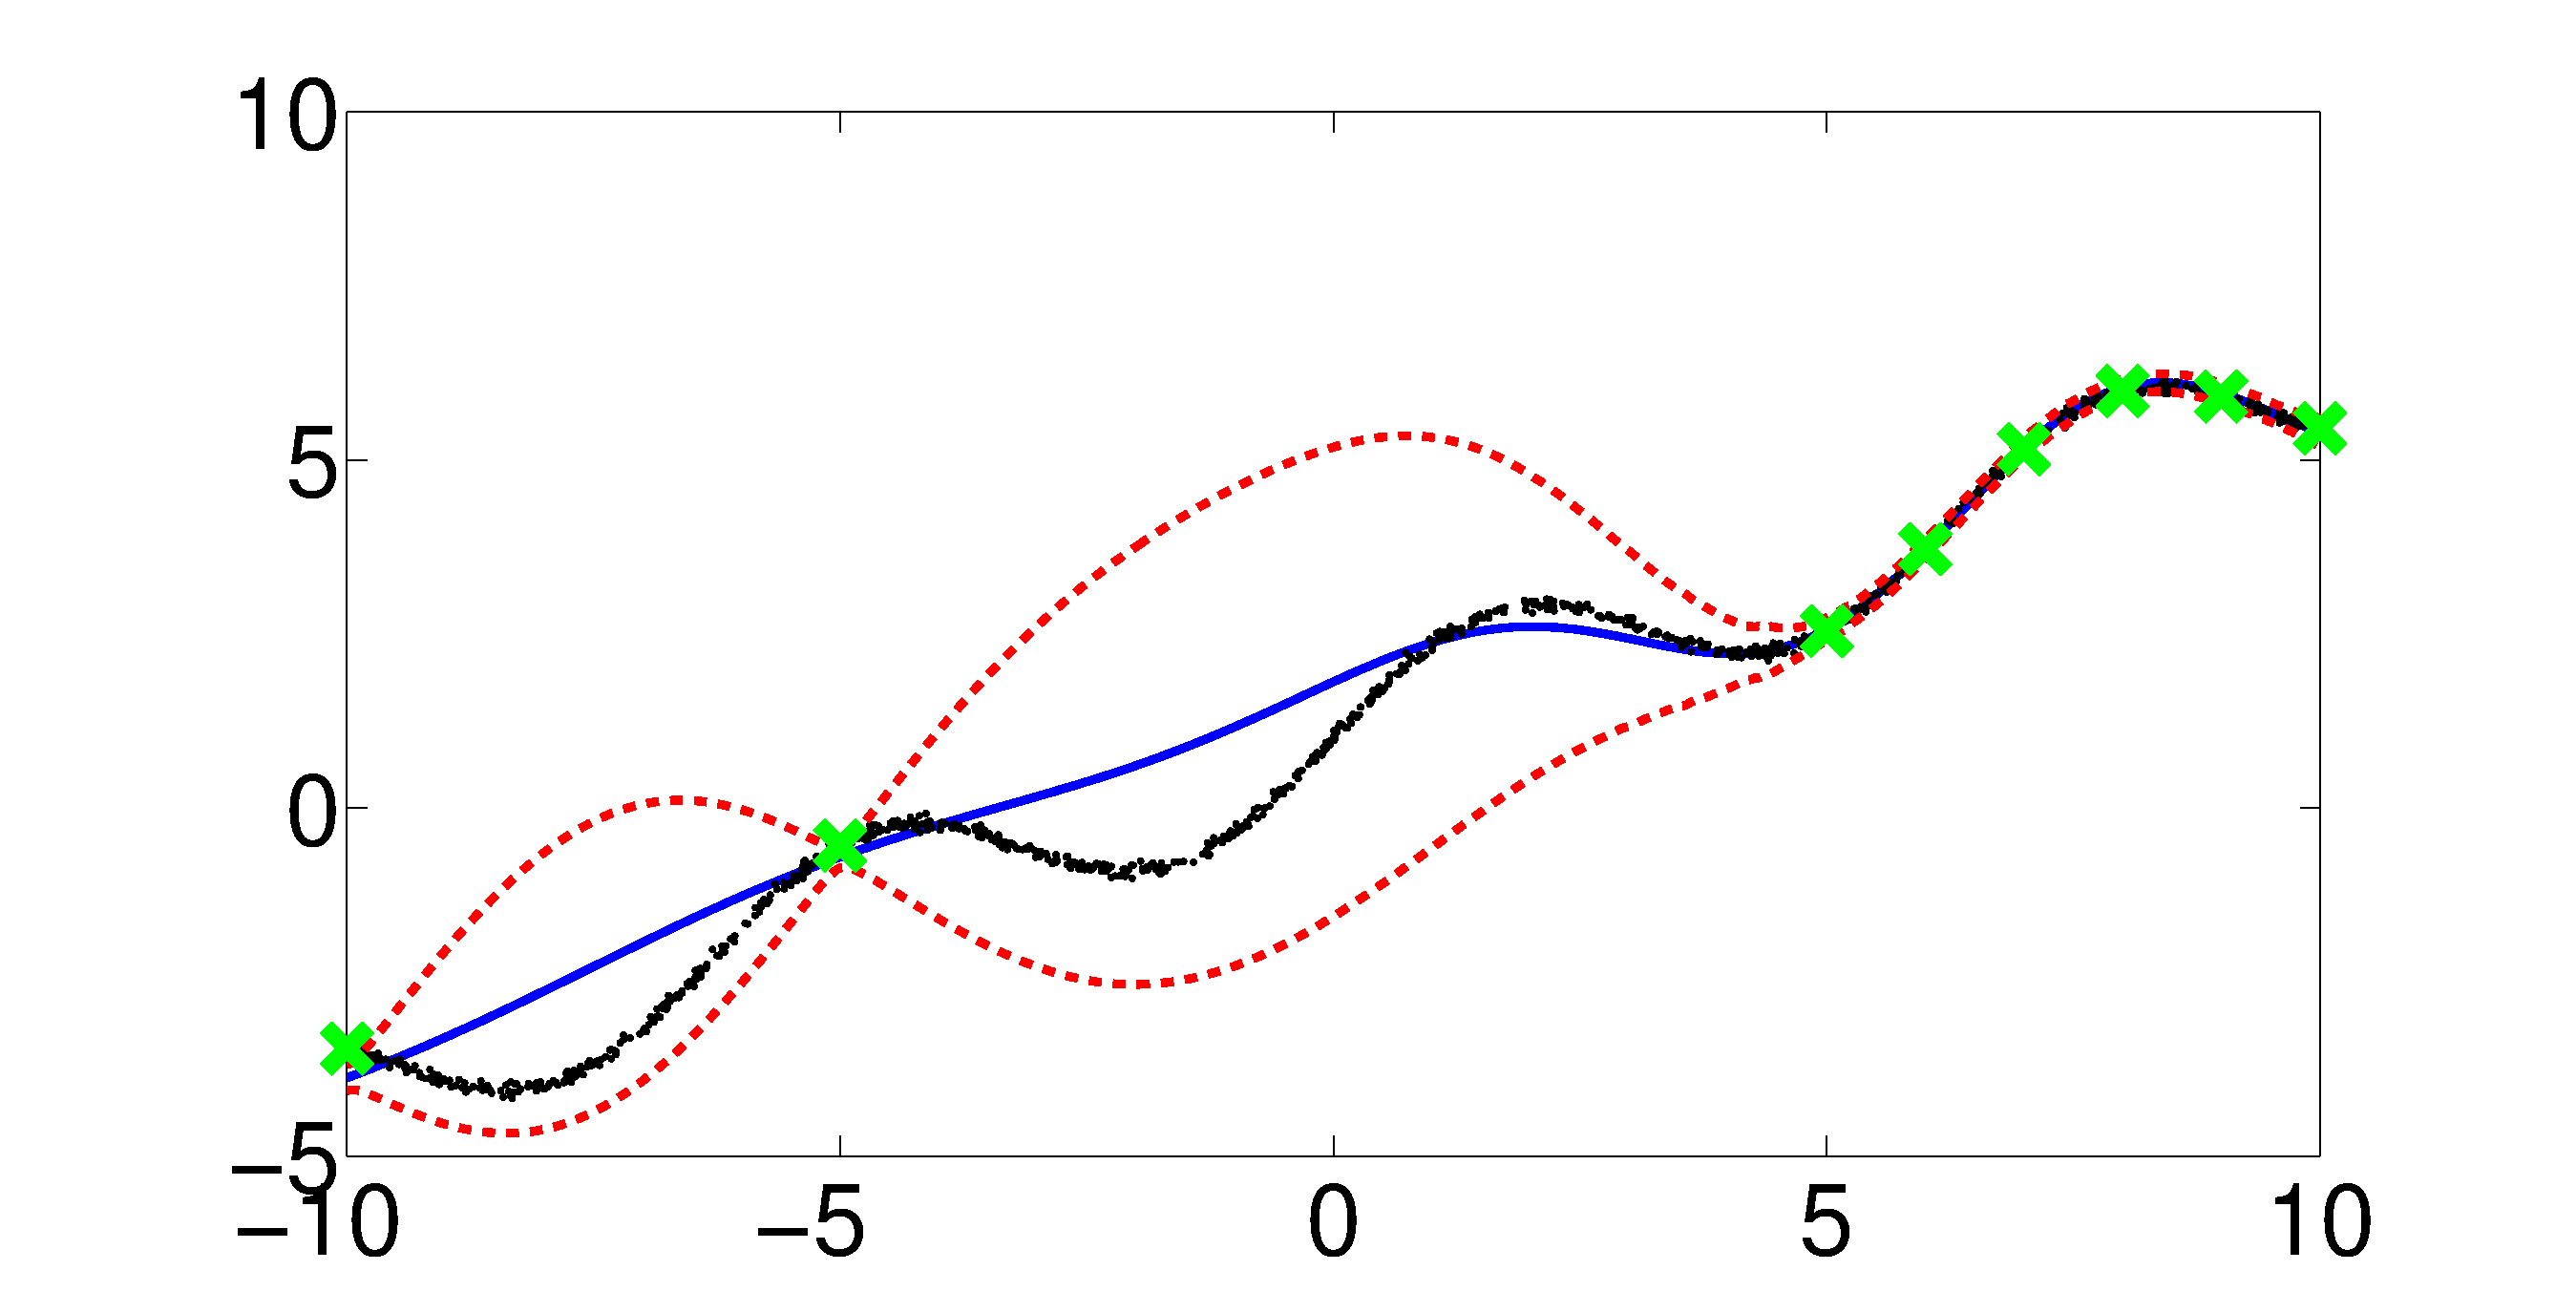
\includegraphics[width=\textwidth,trim=2.5cm 0cm 2.5cm 0.5cm,clip]
      {./sgp/pics/pred_lanc_diag}
      \caption{Lanczos with diagonal correction}
      \label{fig:pred_lanc_diag}
    \end{subfigure}
    \begin{subfigure}{0.46\textwidth}
      \centering
      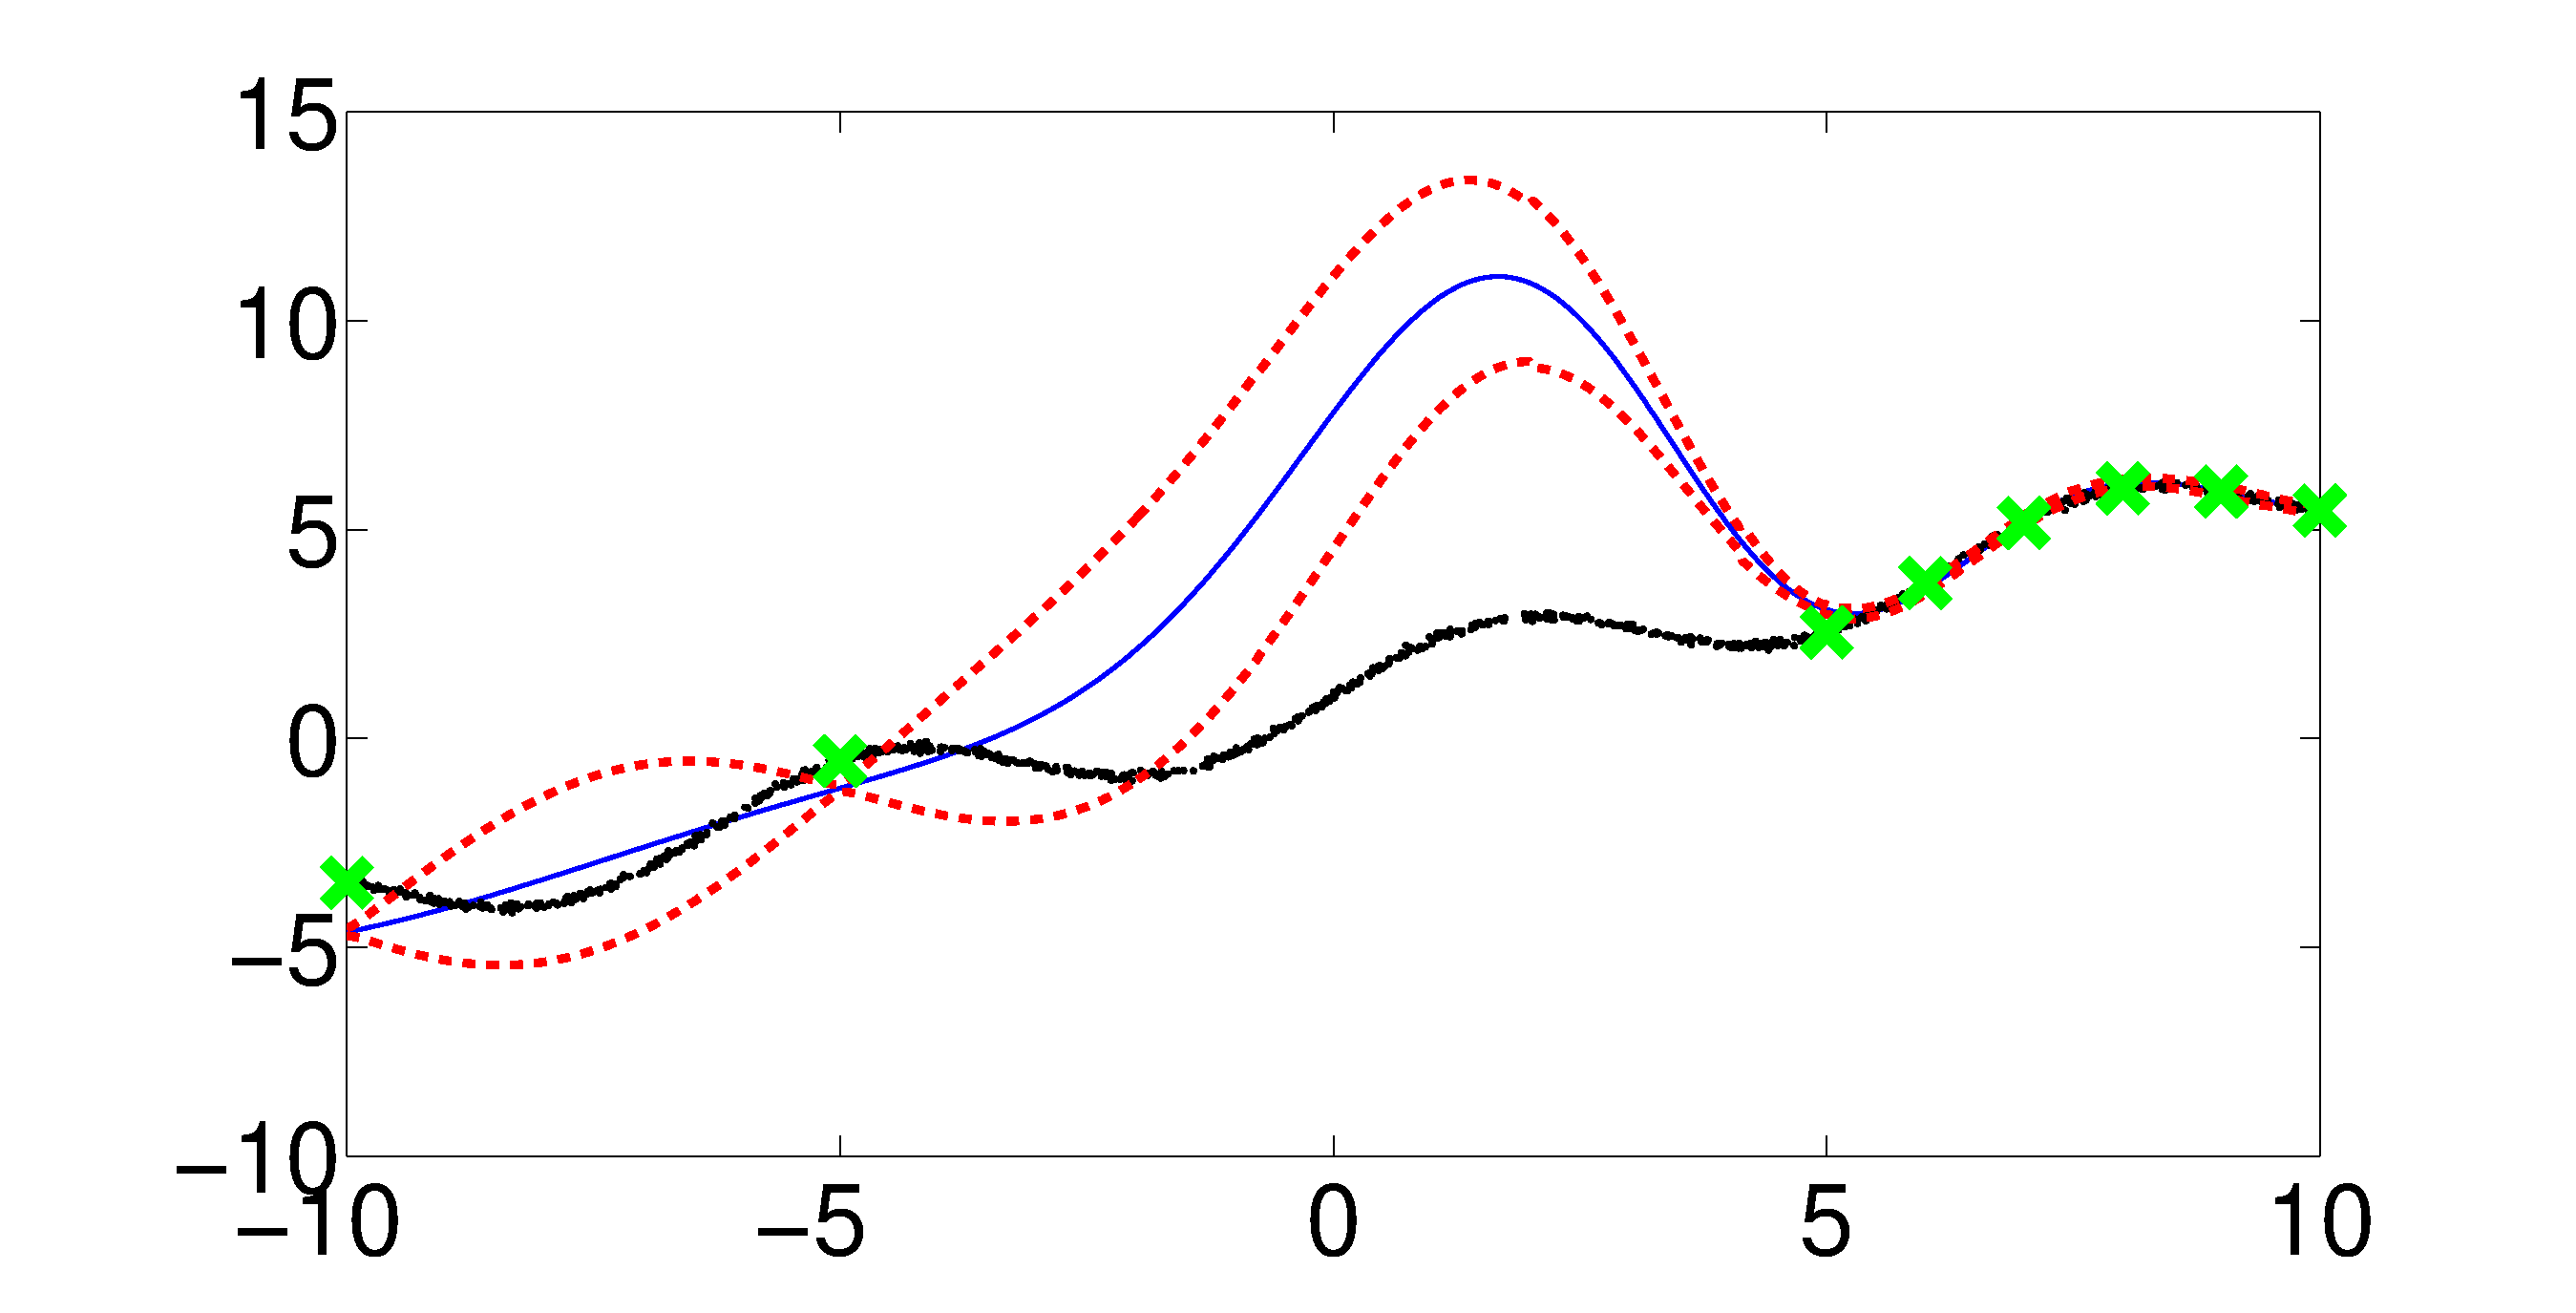
\includegraphics[width=\textwidth,trim=2.5cm 0cm 2.5cm 0.5cm,clip]
      {./sgp/pics/pred_lanc_nodiag}
      \caption{Lanczos without diagonal correction}
      \label{fig:pred_lanc_nodiag}
    \end{subfigure}
    \begin{subfigure}{0.46\textwidth}
      \centering
      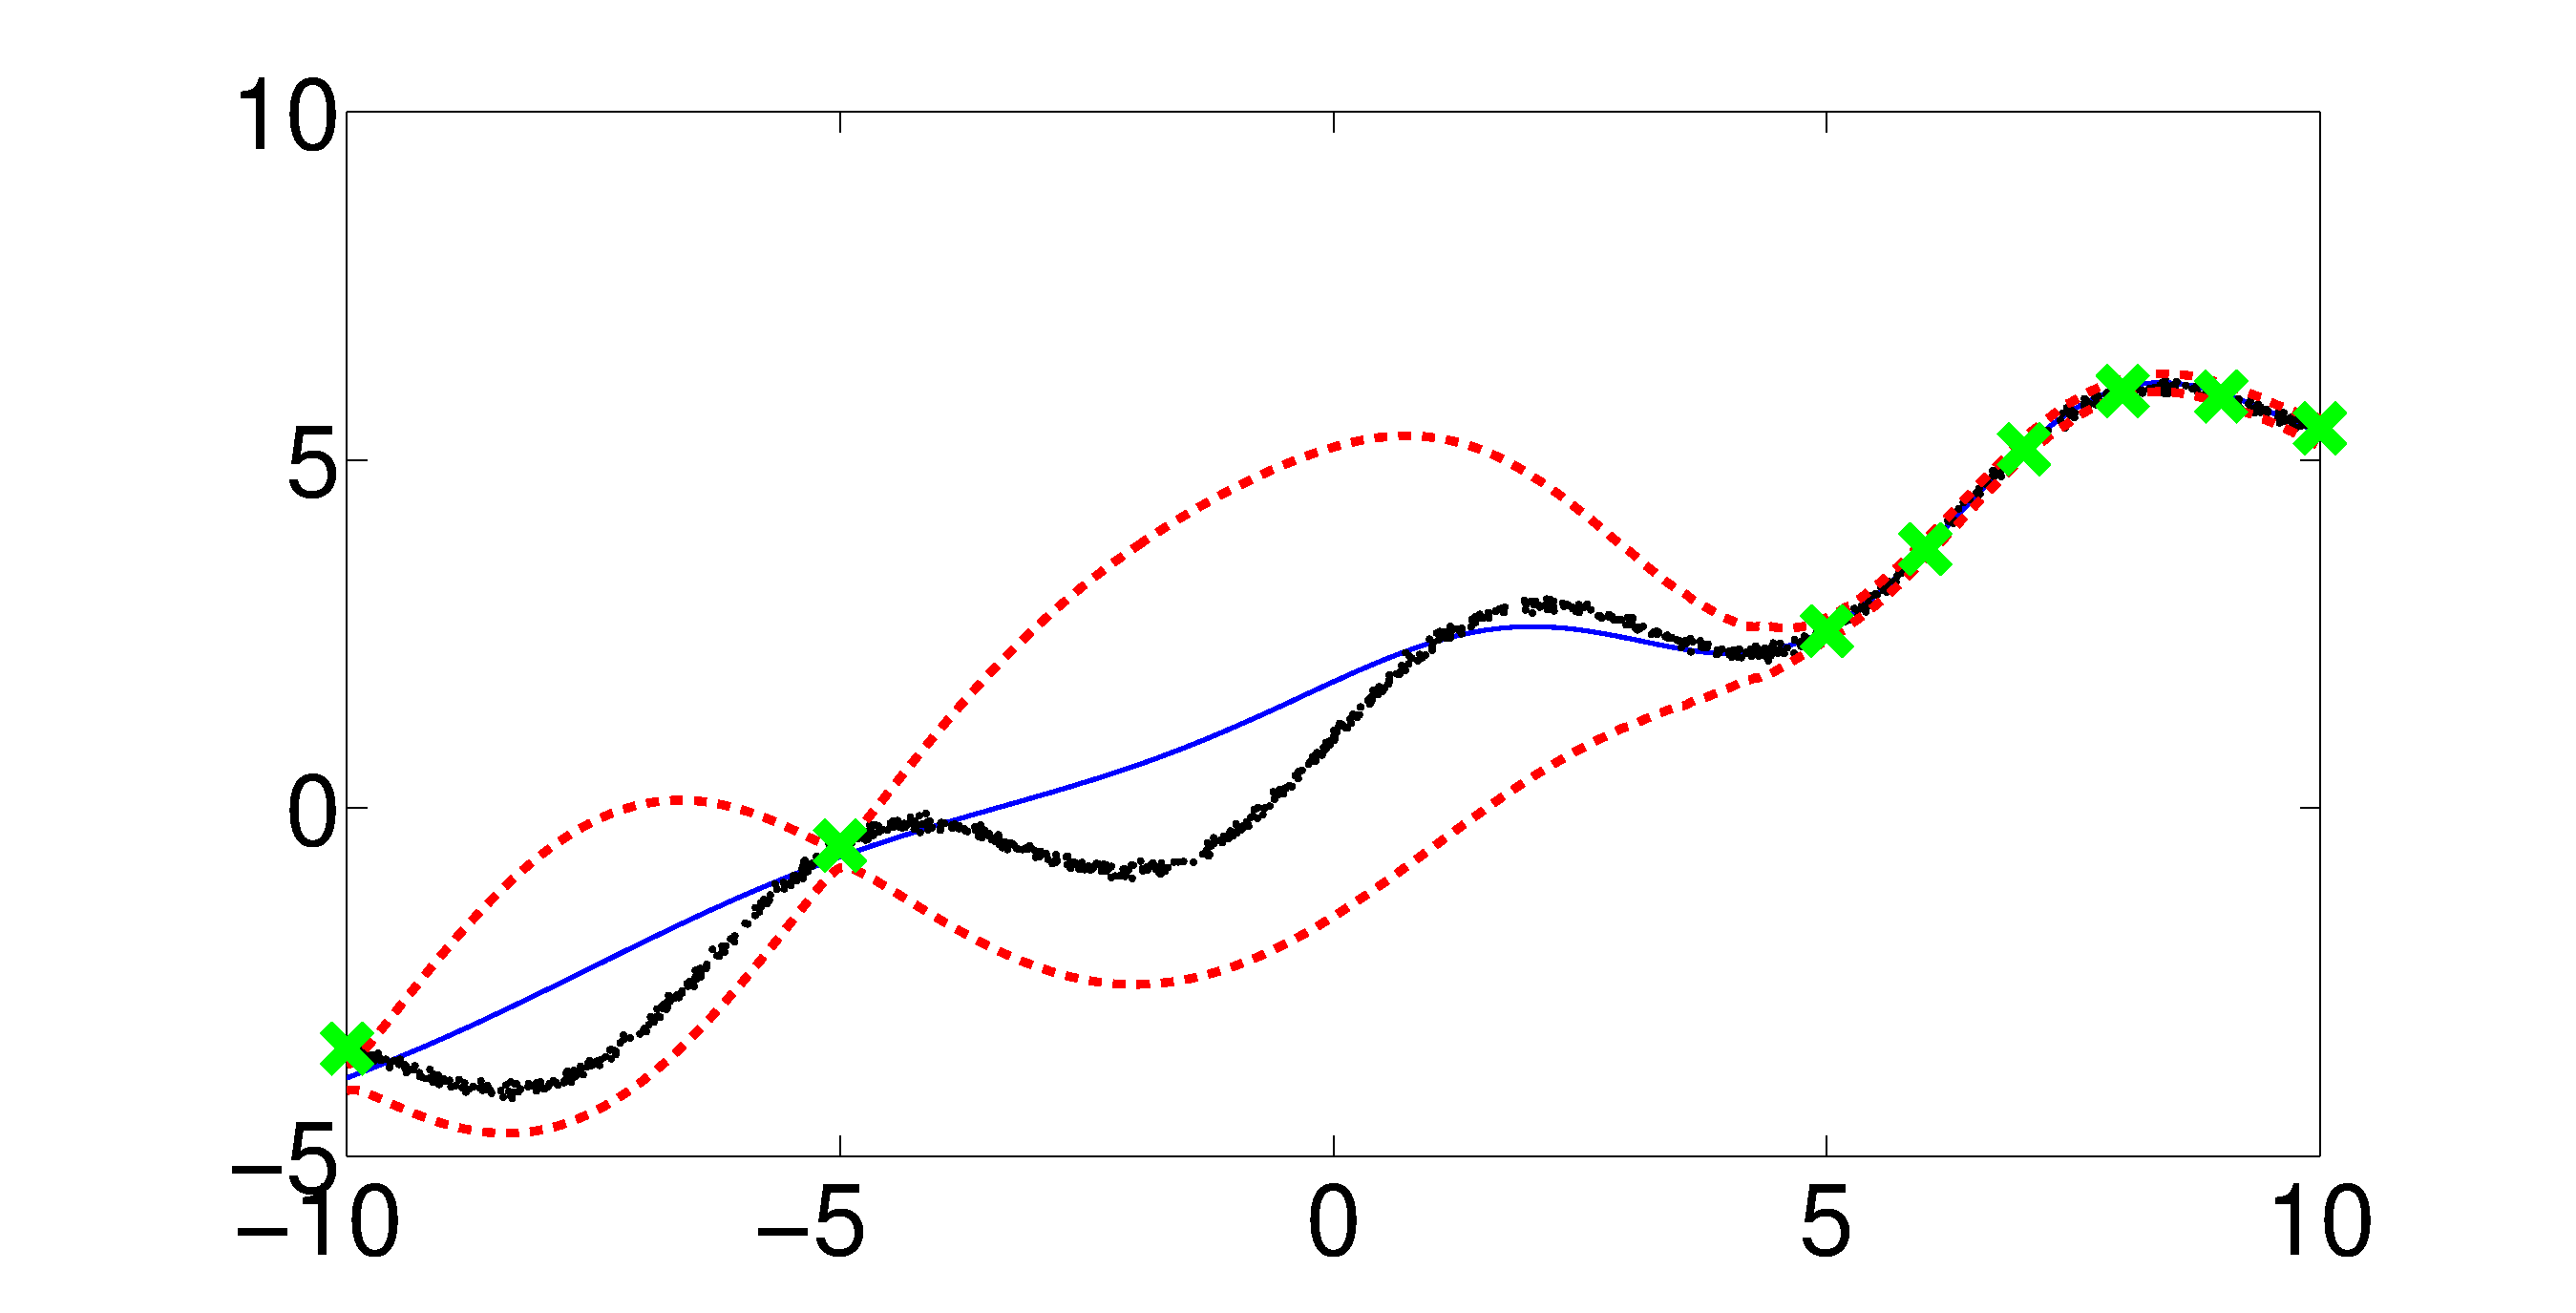
\includegraphics[width=\textwidth,trim=2.5cm 0cm 2.5cm 0.5cm,clip]
      {./sgp/pics/pred_cheb_diag}
      \caption{Chebyshev with diagonal correction}
      \label{fig:pred_cheb_diag}
    \end{subfigure}
    \begin{subfigure}{0.46\textwidth}
      \centering
      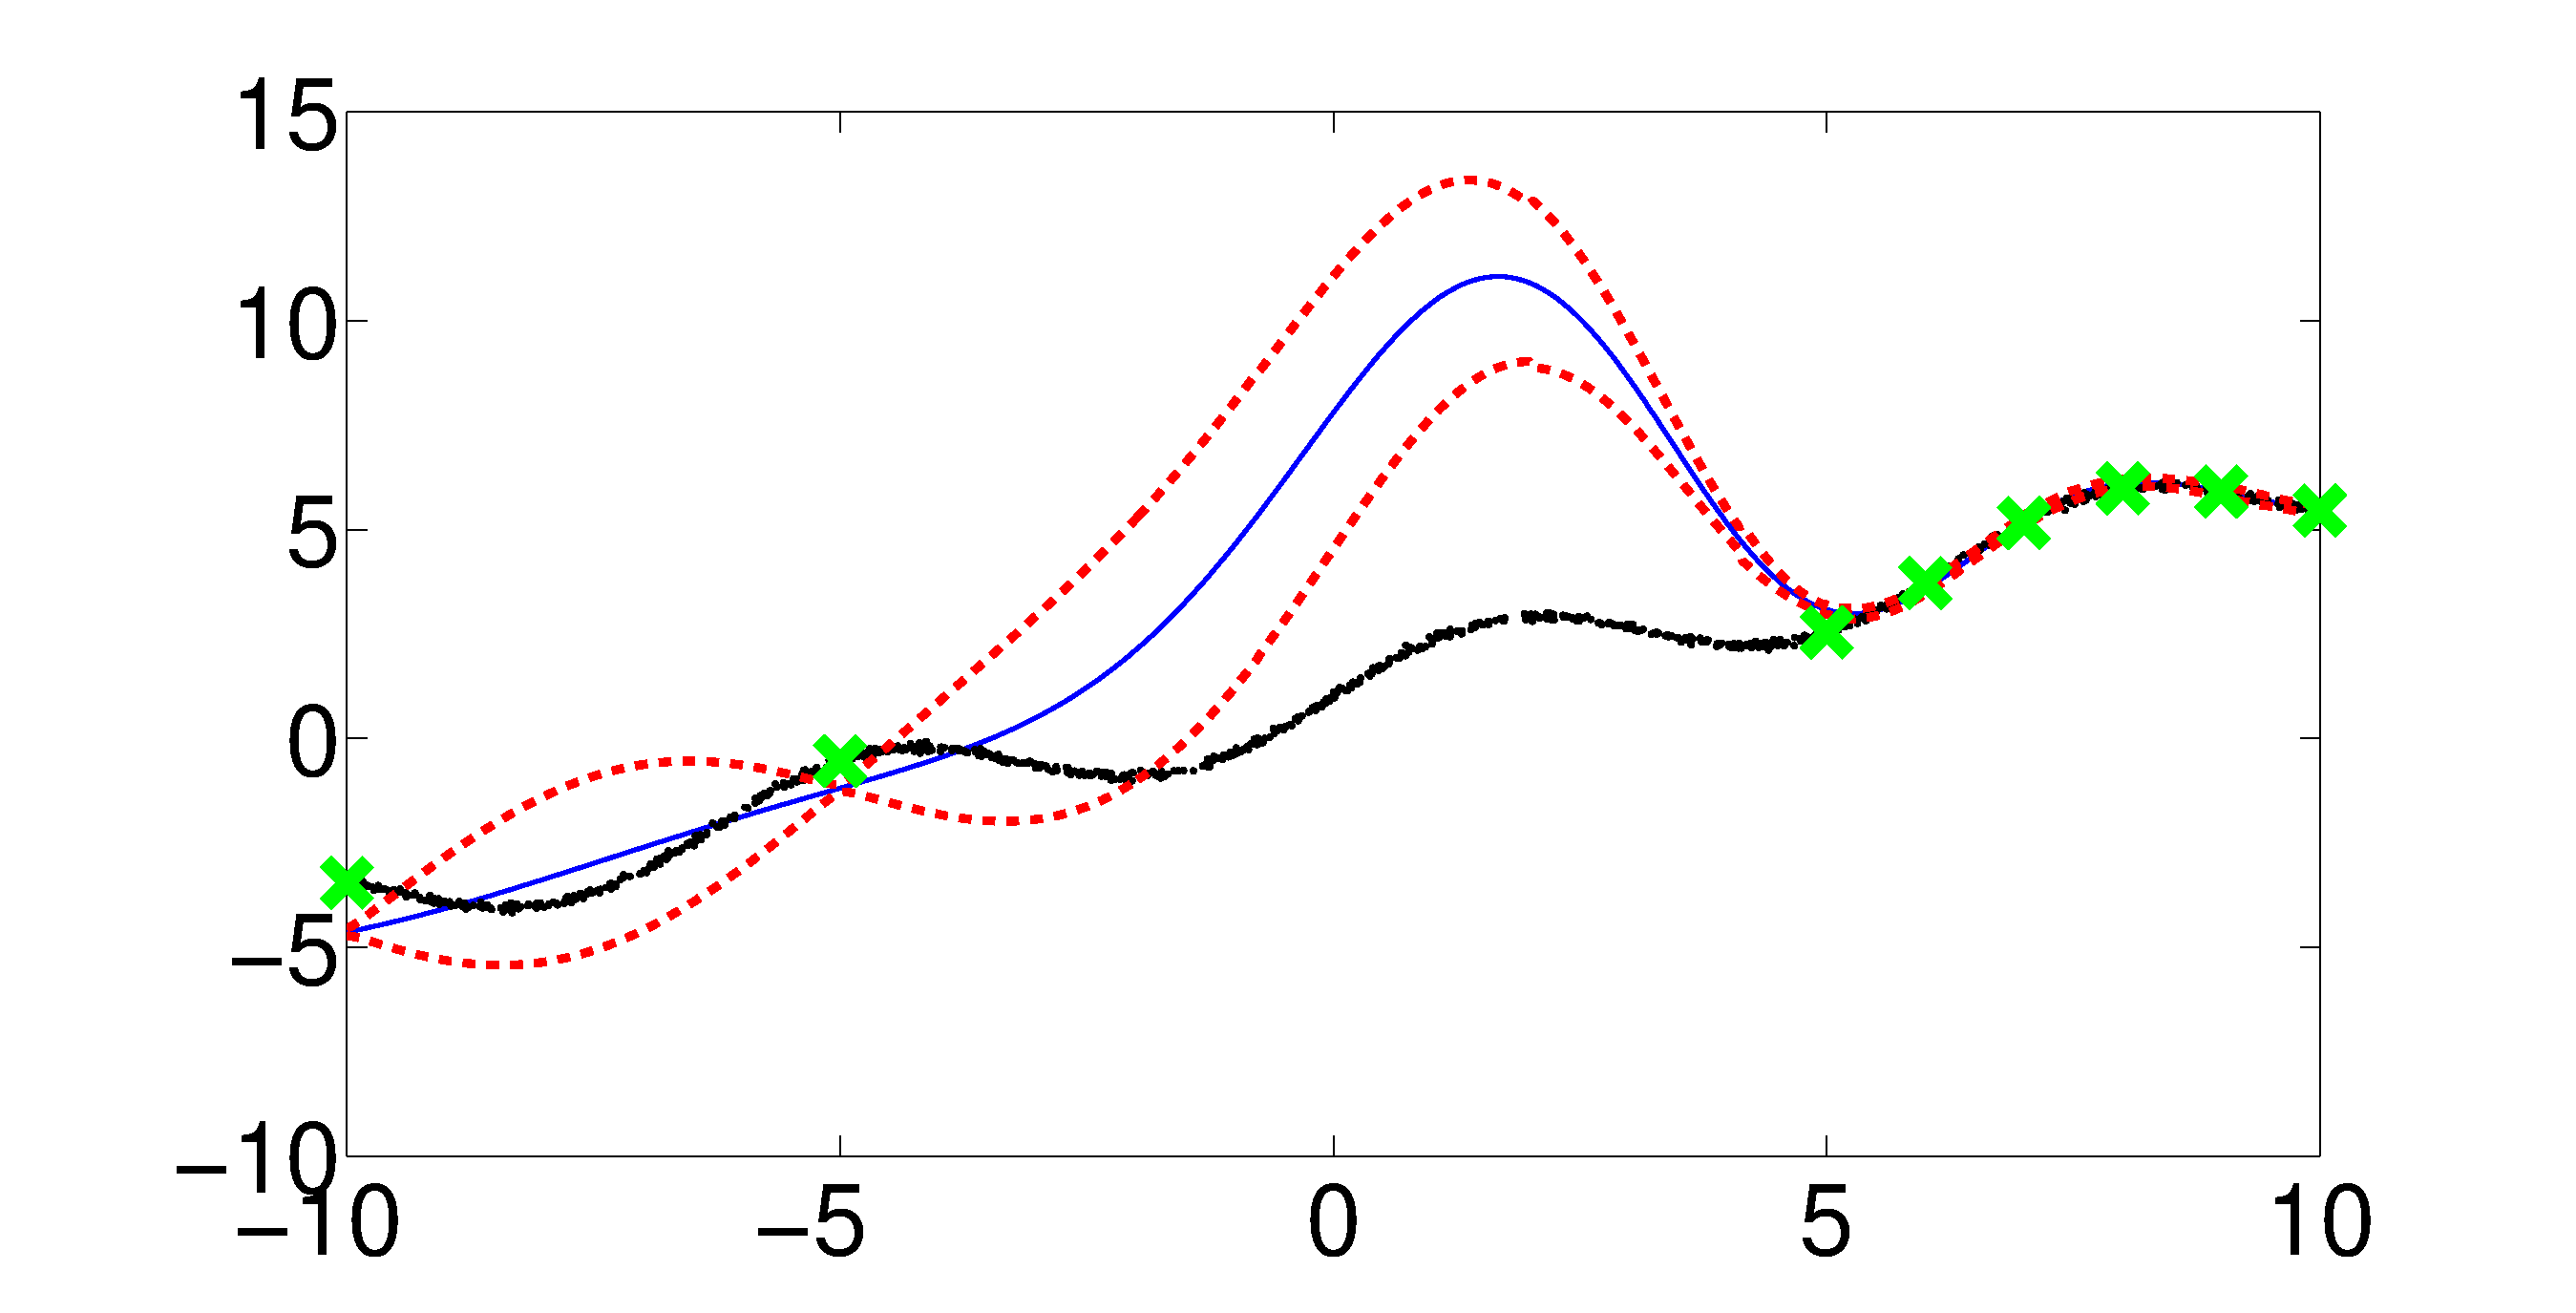
\includegraphics[width=\textwidth,trim=2.5cm 0cm 2.5cm 0.5cm,clip]
      {./sgp/pics/pred_cheb_nodiag}
      \caption{Chebyshev without diagonal correction}
      \label{fig:pred_cheb_nodiag}
    \end{subfigure}
    \begin{subfigure}{0.46\textwidth}
      \centering
      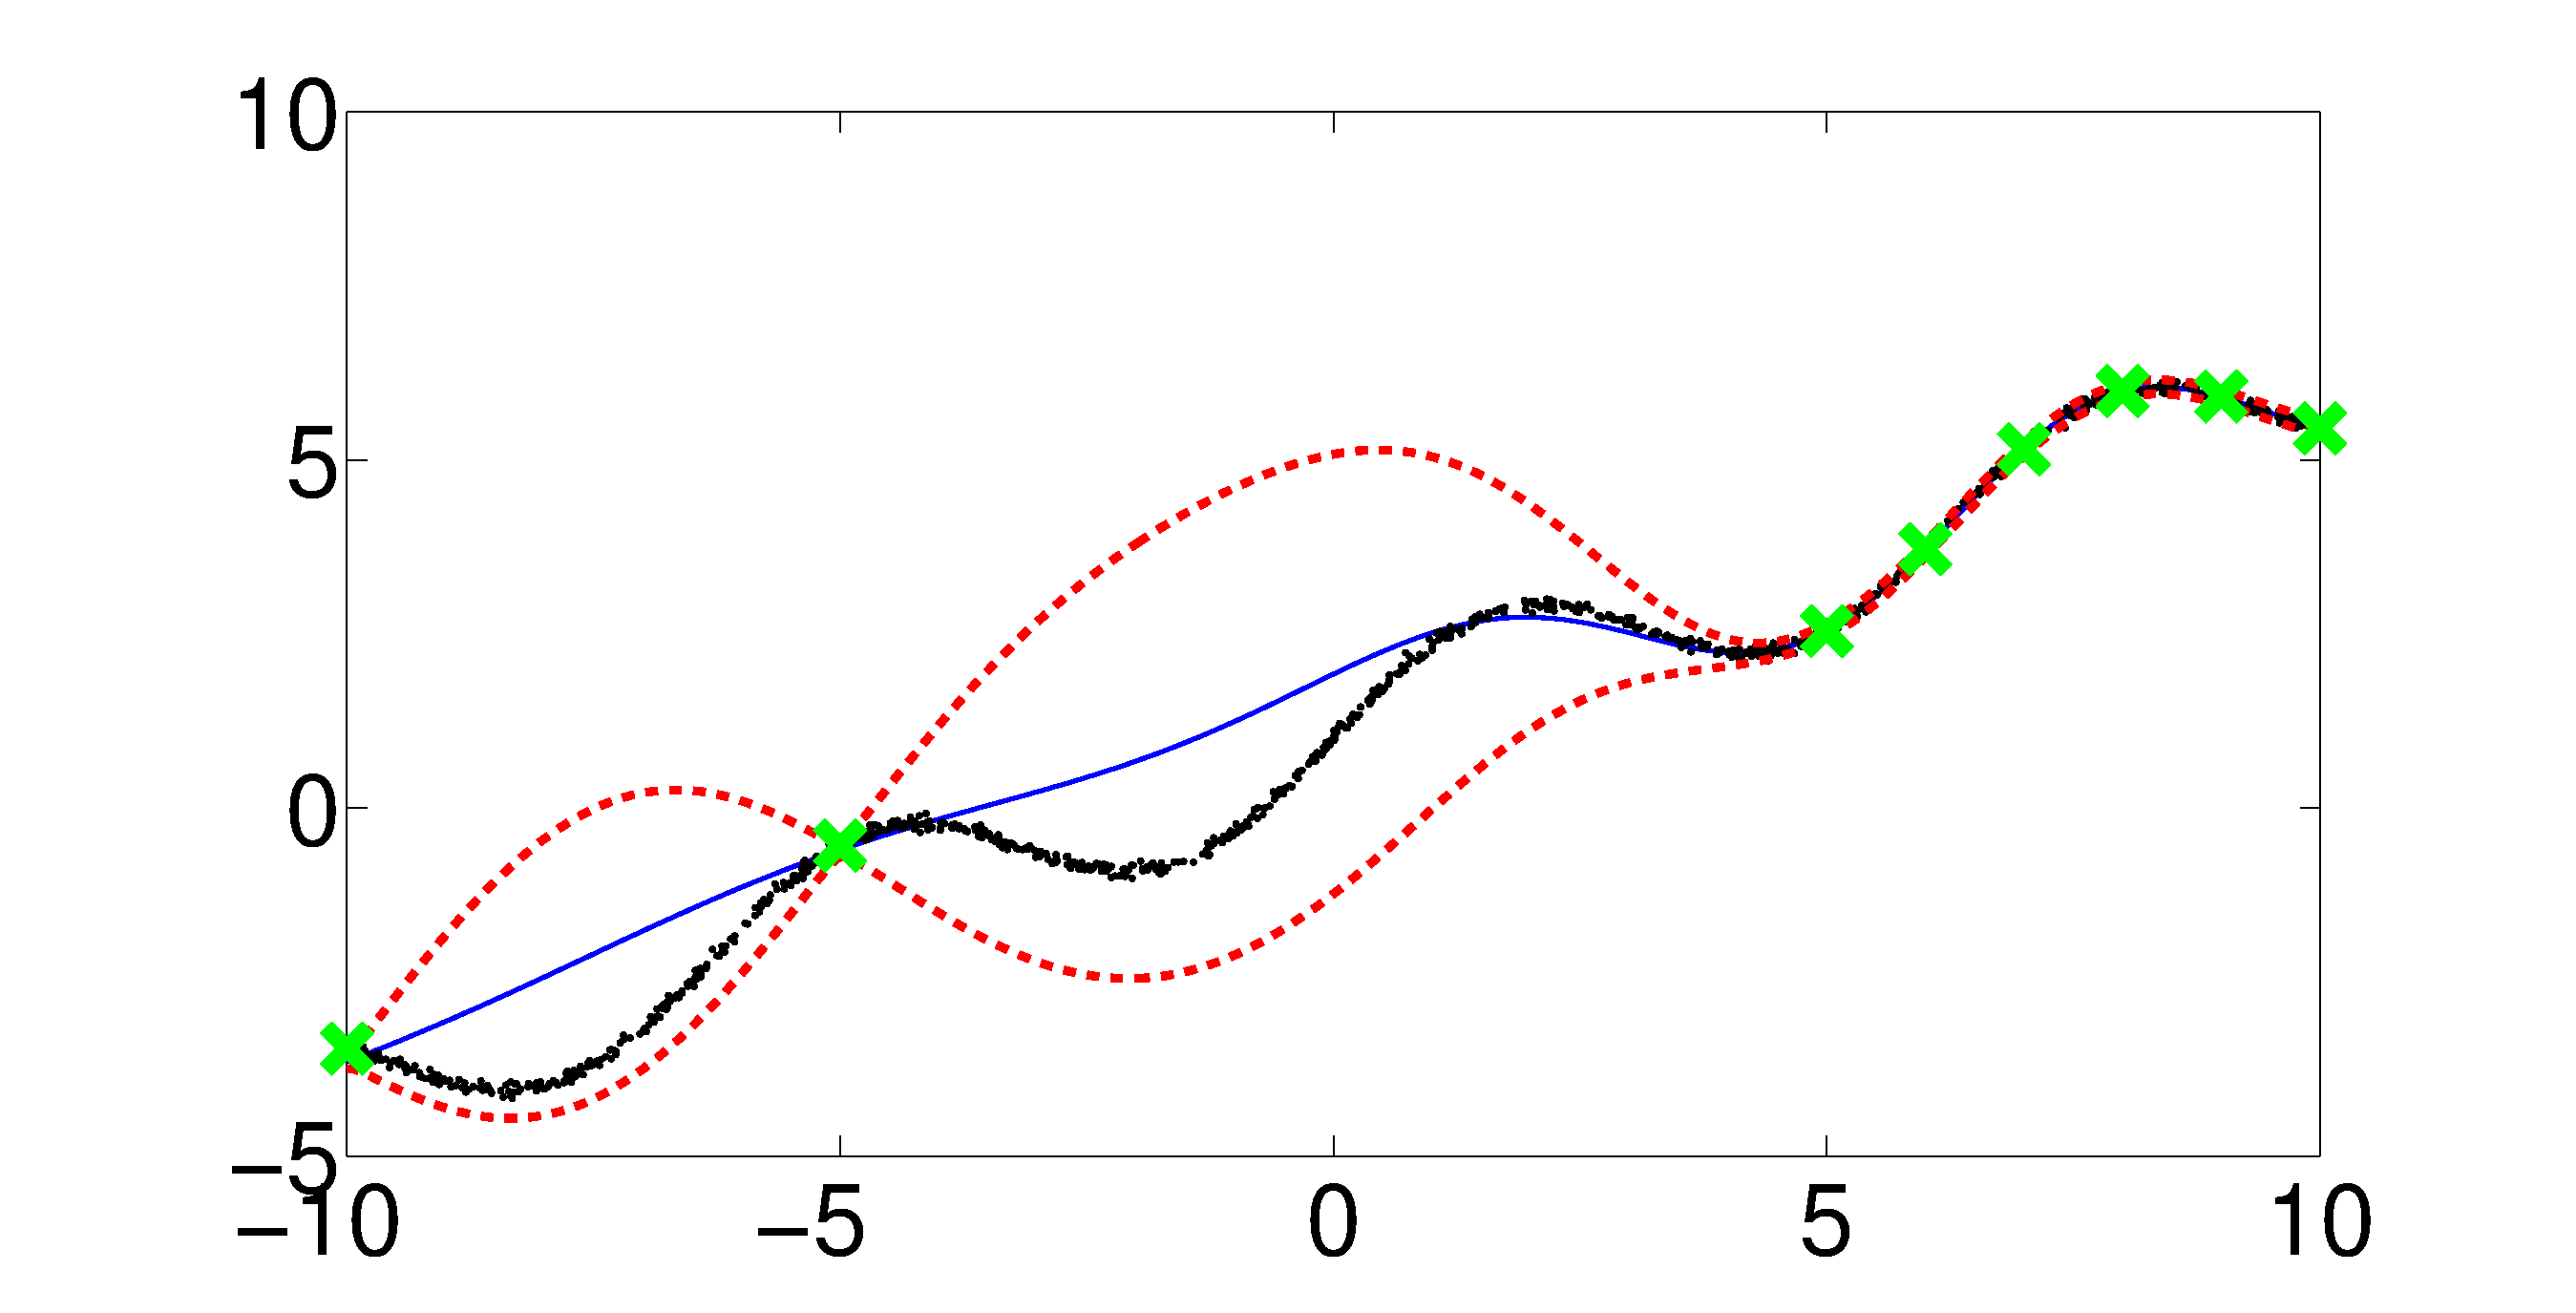
\includegraphics[width=\textwidth,trim=2.5cm 0cm 2.5cm 0.5cm,clip]
      {./sgp/pics/pred_fitc}
      \caption{FITC}
      \label{fig:pred_fitc}
    \end{subfigure}
    \begin{subfigure}{0.46\textwidth}
      \centering
      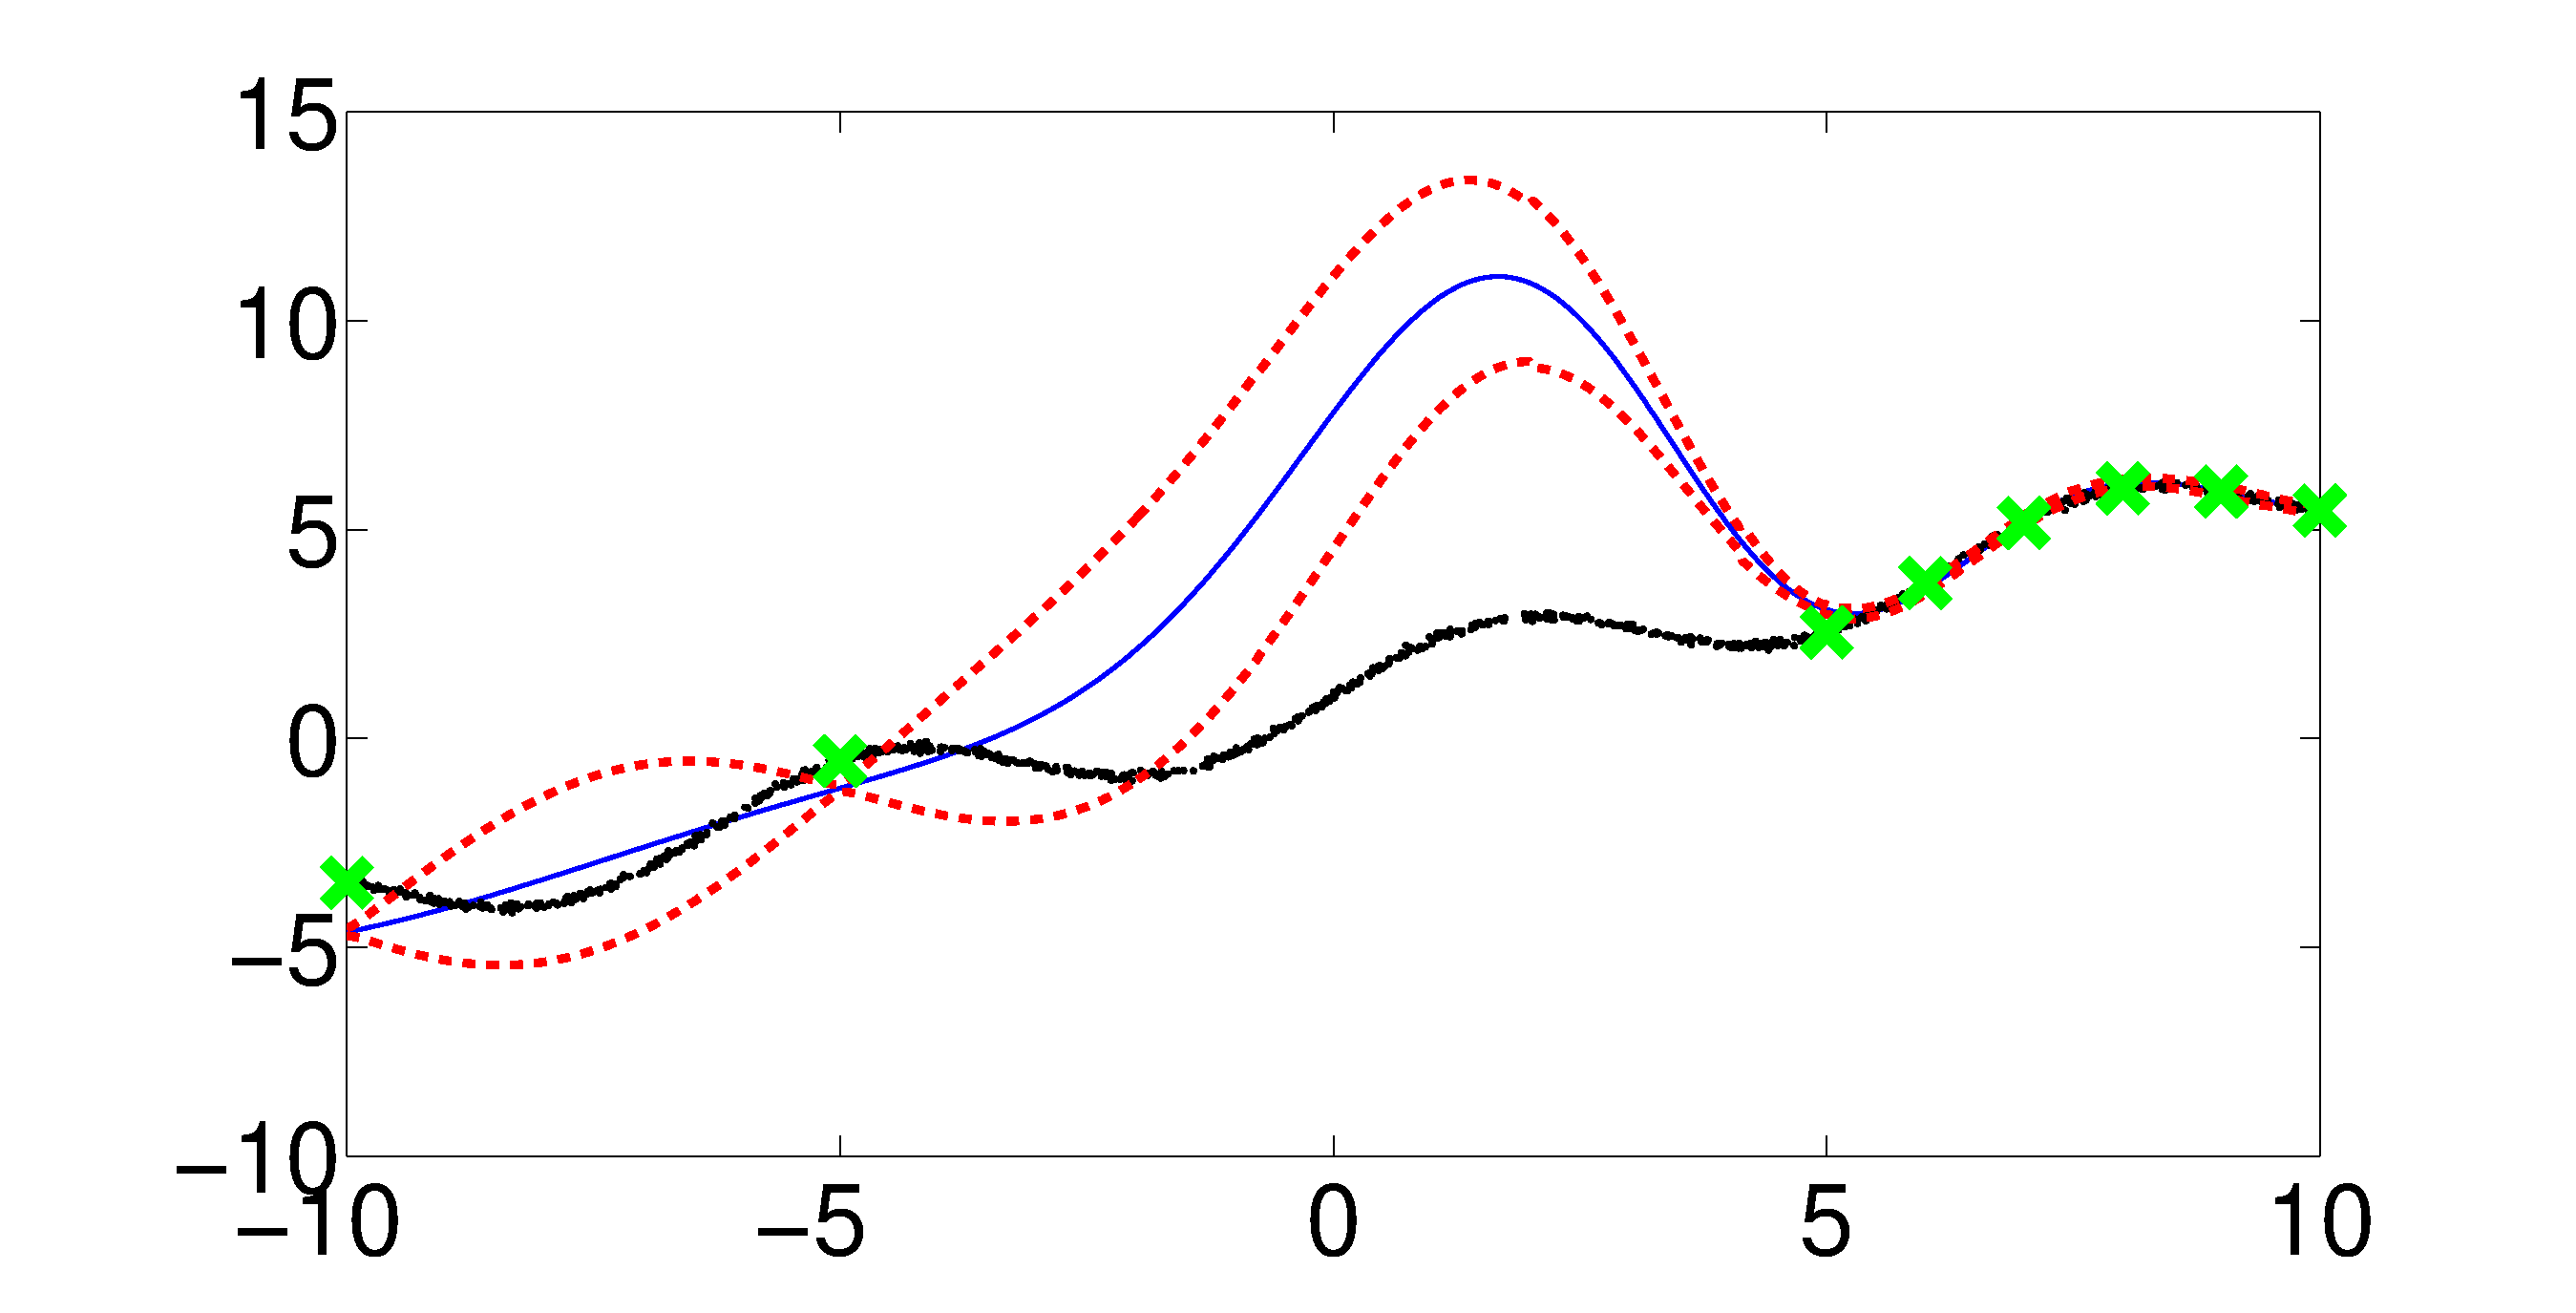
\includegraphics[width=\textwidth,trim=2.5cm 0cm 2.5cm 0.5cm,clip]
      {./sgp/pics/pred_sceig}
      \caption{Scaled eigenvalue method}
      \label{fig:pred_sceig}
    \end{subfigure}
    \caption{Example that shows how important diagonal correction can be for
    some kernels. The Mat\'ern\hyp{}$3/2$ kernel was used to fit the data given
    by the black dots. This data was generated from the function $f(x) = 1 + x/2
    + \sin(x)$ to which we added normally distributed noise with standard
    deviation $0.05$. We used the exact method to find the optimal
    hyper\hyp{}parameters and used these hyper\hyp{}parameters to study the
    different behavior of the predictive uncertainties when the inducing points
    are given by the green crosses. The solid blue line is the predictive mean
    and the dotted red lines shows a confidence interval of two standard
    deviations.}\label{fig:diag_correction}
  \end{center}
\end{figure}

It is clear that Lanczos and Chebyshev are too confident in the predictive mean
when diagonal correction is not used, while the predictive uncertainties agree
well with FITC when diagonal correction is used. The scaled eigenvalue method
cannot be used efficiently with diagonal correction and we see that this leads
to predictions similar to Lanczos and Chebyshev without diagonal correction. The
flexibility of being able to use diagonal correction with Lanczos and Chebyshev
makes these approaches very appealing.

\subsection{Surrogate Log Determinant Approximation}
\label{sup:surrlogdetapprox}

The point of this experiment is to illustrate how accurate the level\hyp{}curves
of the surrogate model are compared to the level\hyp{}curves of the true log
determinant. We consider the RBF and the Mat\'ern\hyp{}$3/2$ kernels and the
same datasets that we considered in \ref{sup:1dcross}. We fix $s_f=1$ and study
how the level curves compare when we vary $\ell$ and $\sigma$. Building the
surrogate with all three hyper\hyp{}parameters produces similar results, but
requires more design points. We use $50$ design points to construct a cubic RBF
with a linear tail. The values of the log determinant and its derivatives
are computed with Lanczos. It is clear from \cref{fig:level_curves} that the
surrogate model does a good job approximating the log determinant for both
kernels.

\begin{figure}[ht]
  \begin{center}
    \begin{subfigure}{0.46\textwidth}
      \centering
      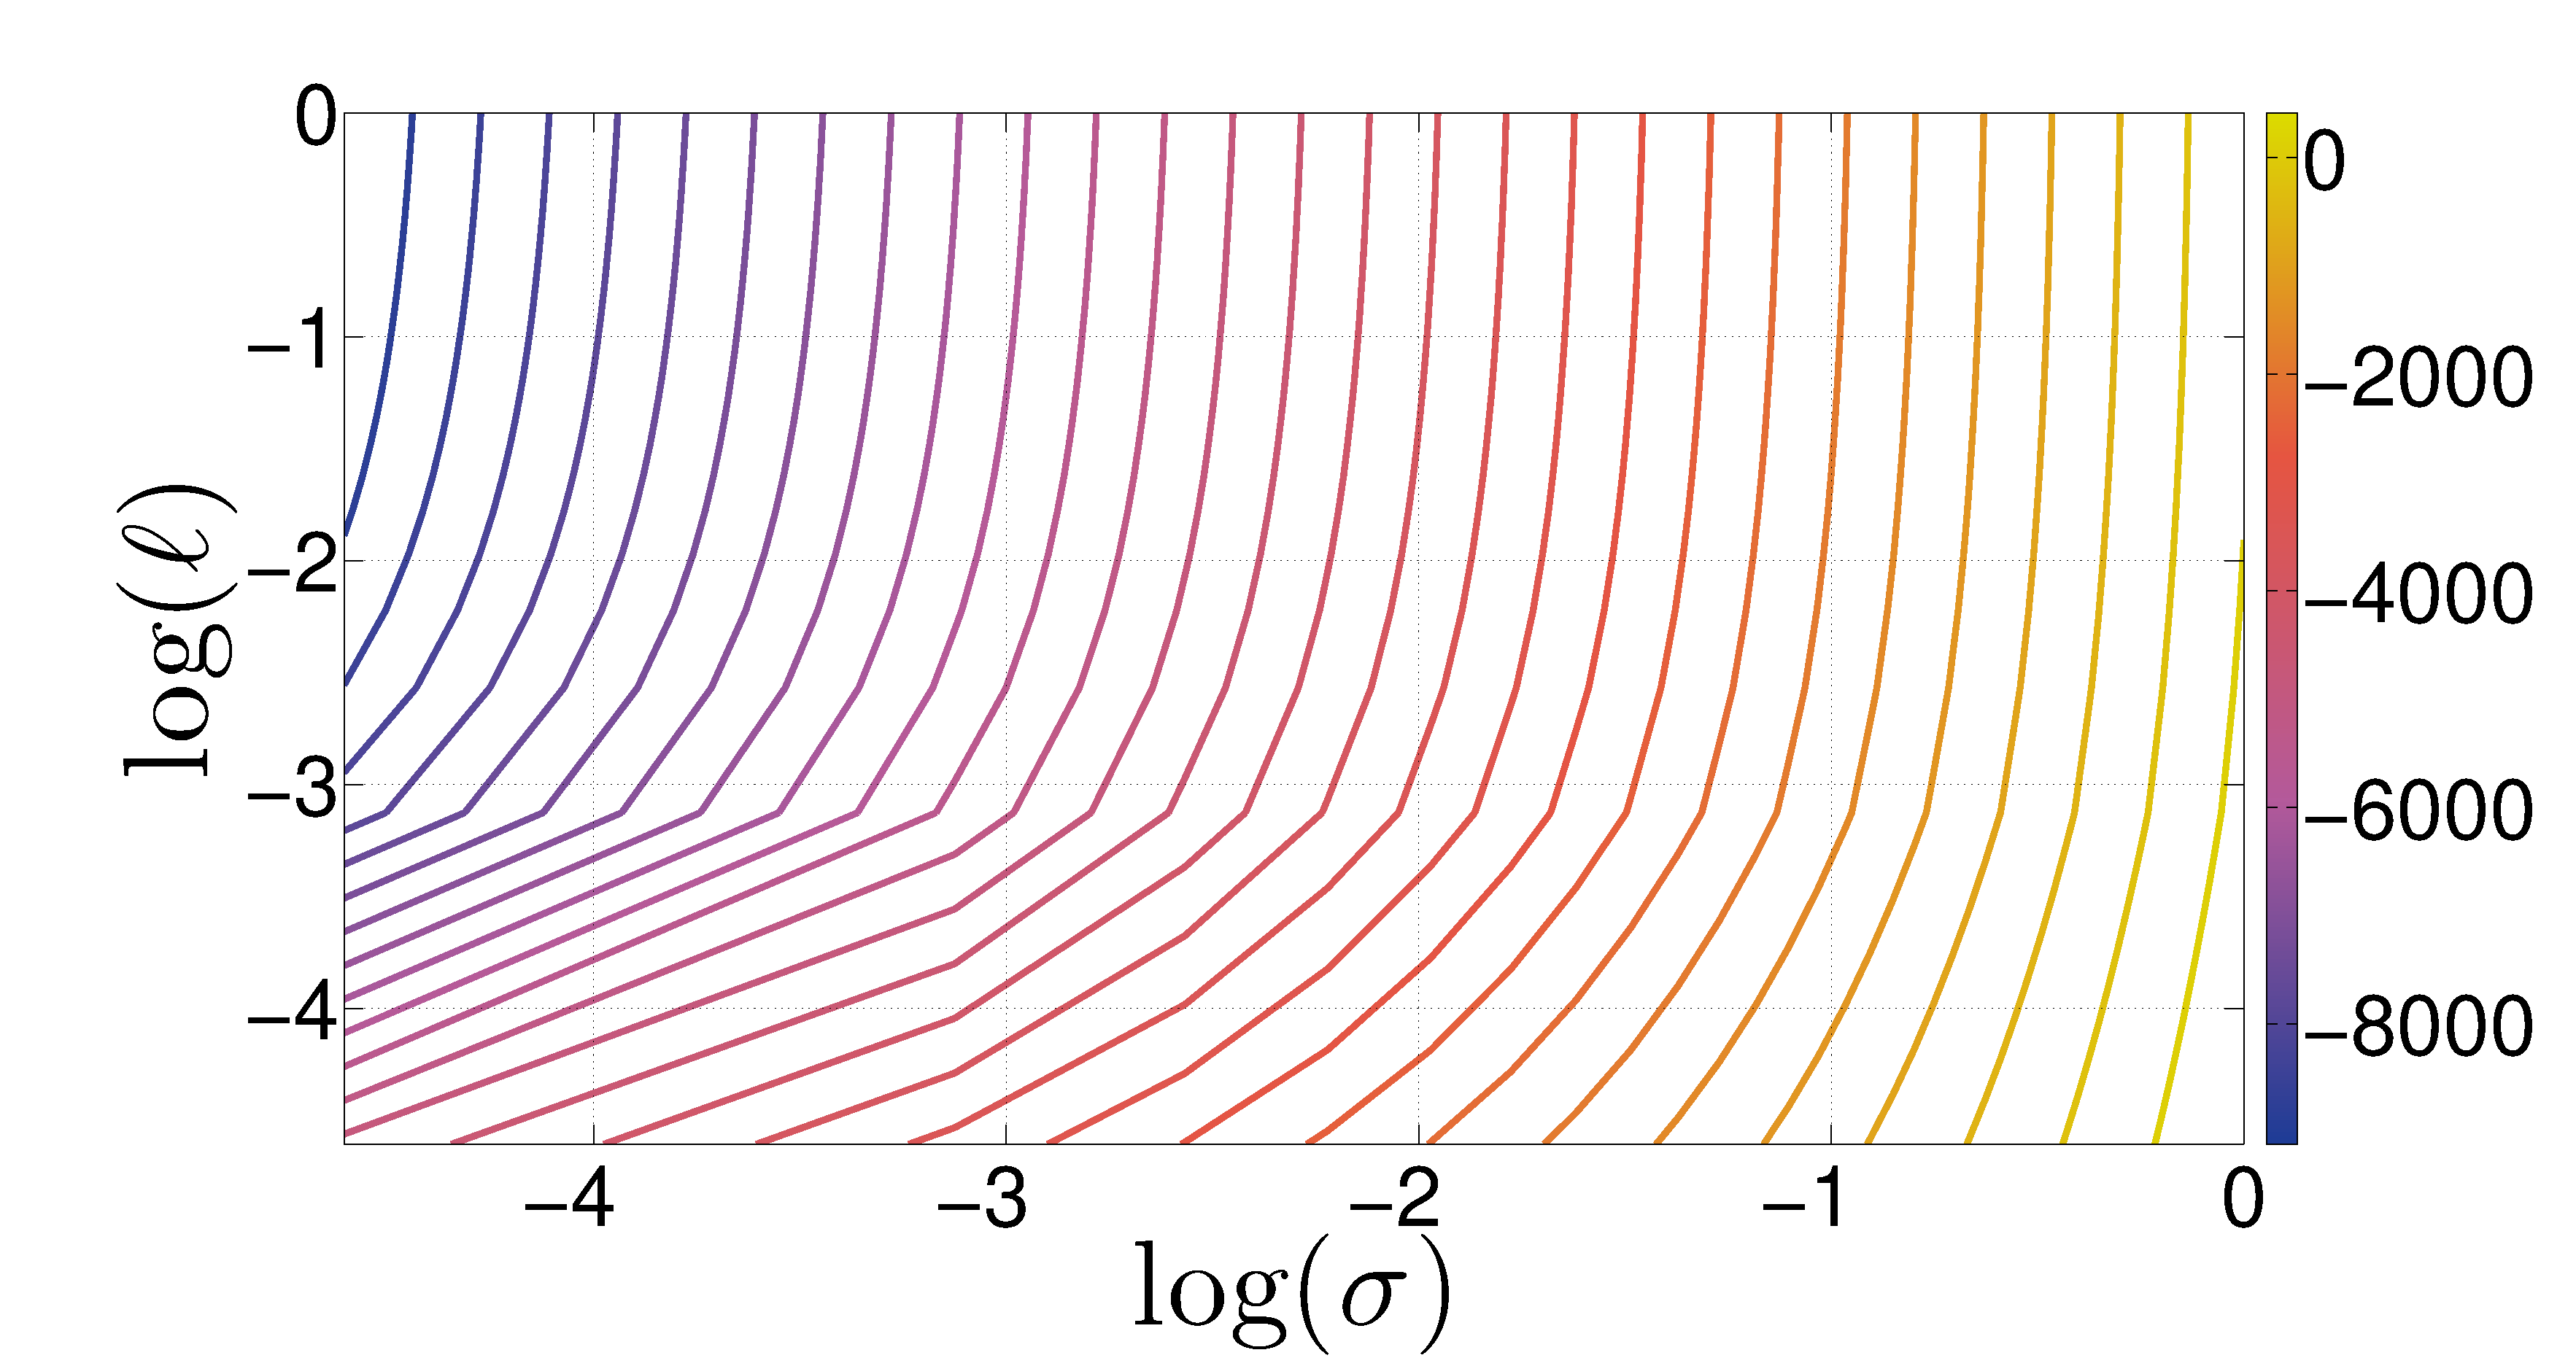
\includegraphics[width=\textwidth,trim=2.5cm 0cm 0.5cm 1.5cm,clip]
      {./sgp/pics/level_curves_rbf_exact}
      \caption{RBF exact}
      \label{fig:level_rbf_exact}
    \end{subfigure}
    \begin{subfigure}{0.46\textwidth}
      \centering
      \includegraphics[width=\textwidth,trim=2.5cm 0cm 0.5cm 1.5cm,clip]
      {./sgp/pics/level_curves_Matern3_2_exact}
      \caption{Mat\'ern\hyp{}$3/2$ exact}
      \label{fig:level_Matern3_2_exact}
    \end{subfigure}
    \begin{subfigure}{0.46\textwidth}
      \centering
      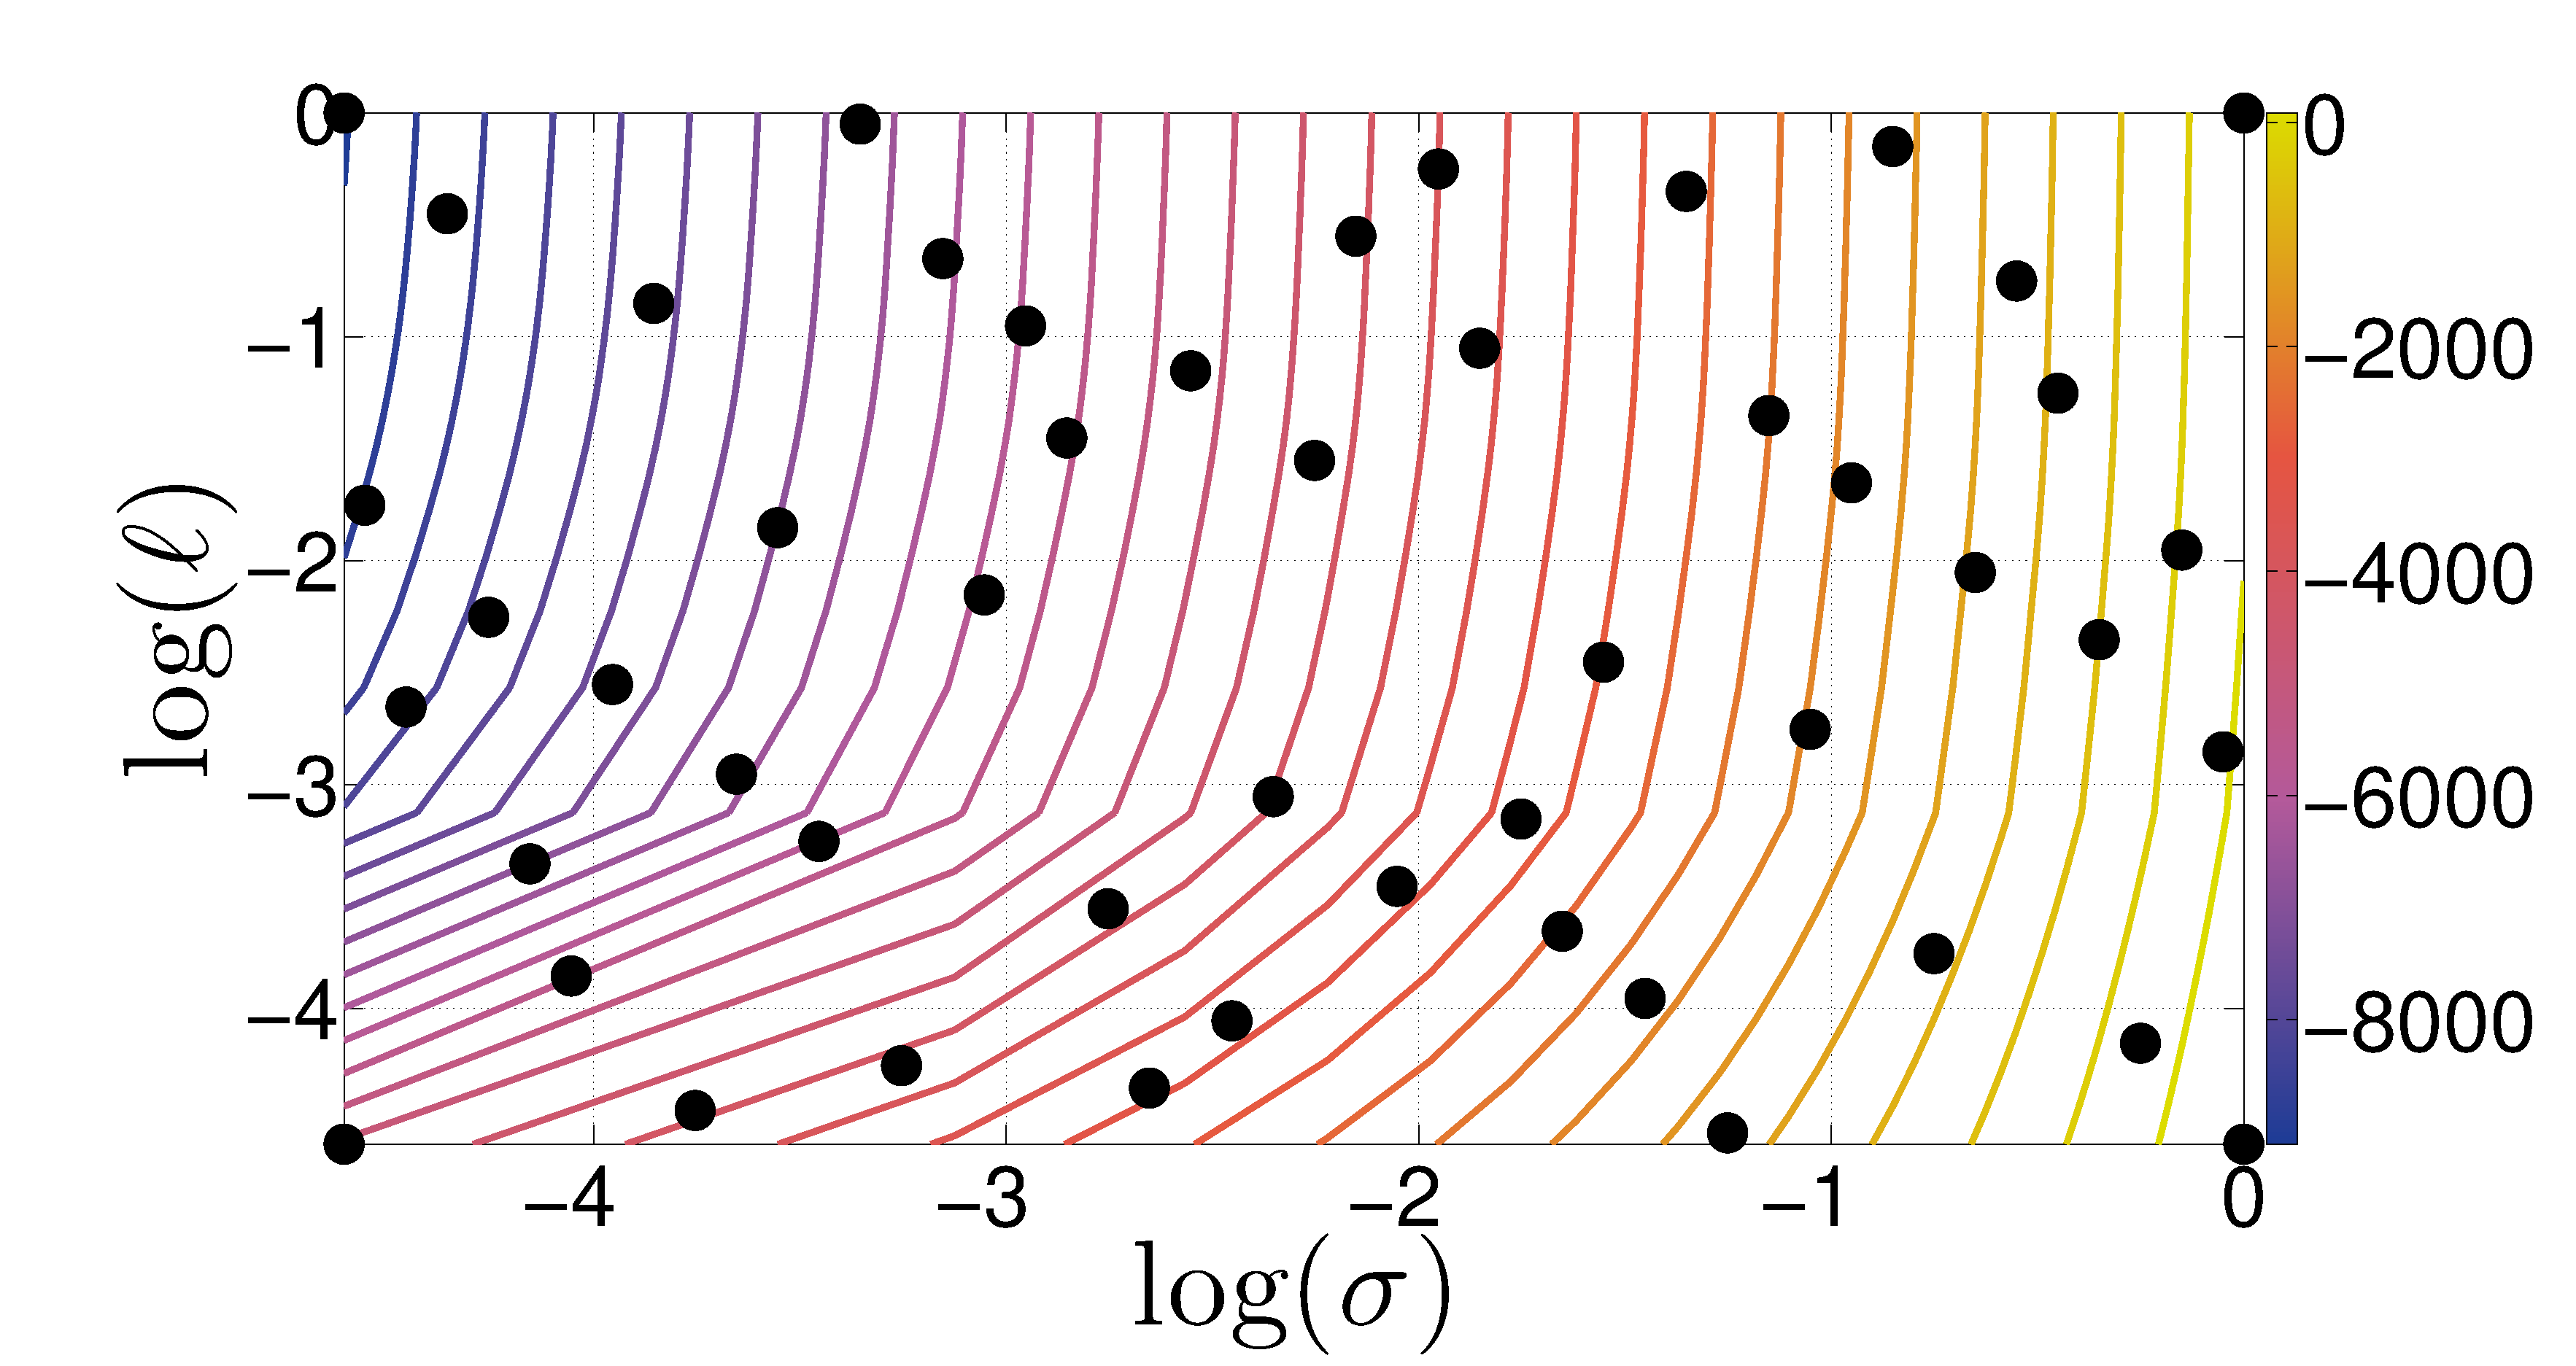
\includegraphics[width=\textwidth,trim=2.5cm 0cm 0.5cm 1.5cm,clip]
      {./sgp/pics/level_curves_rbf_surrogate}
      \caption{RBF surrogate}
      \label{fig:level_rbf_surrogate}
    \end{subfigure}
    \begin{subfigure}{0.46\textwidth}
      \centering
      \includegraphics[width=\textwidth,trim=2.5cm 0cm 0.5cm 1.5cm,clip]
      {./sgp/pics/level_curves_Matern3_2_surrogate}
      \caption{Mat\'ern\hyp{}$3/2$ surrogate}
      \label{fig:level_Matern3_2_surrogate}
    \end{subfigure}
    \caption{Level curves of the exact and surrogate approximation of the log
    determinant as a function of $\ell$ and $\sigma$ for the RBF and 
    Mat\'ern\hyp{}$3/2$ kernels. We used $s_f=1$ and the dataset consisted of
    1000 equally spaced points in the interval $[0,4]$. The surrogate model was
    constructed from the points shown with ($\bullet$) and the log determinant
    values were computed using stochastic Lanczos.}\label{fig:level_curves}
  \end{center}
\end{figure}

\subsection{Kernel Hyper-parameter Recovery}\label{sup:hyperrecov}

This experiments tests how well we can recover hyper\hyp{}parameters from data
generated from a GP. We compare Chebyshev, Lanczos, the surrogate, the scaled
eigenvalue method, and FITC. We consider a dataset of $5000$ points generated
from a $\calN(0,2)$ distribution. We use SKI with cubic interpolation and a
total of $2000$ inducing points for Lanczos, Chebyshev, and then scaled
eigenvalue method. FITC was used with $750$ equally spaced points because it has
a longer runtime as a function of the number of inducing points. We consider the
RBF kernel and the Mat\'ern\hyp{}$3/2$ kernel and sample from a GP with ground
truth parameters $(\ell,s_f,\sigma)=(0.01, 0.5, 0.05)$. The GPs for which we try
to recover the hyper\hyp{}parameters were generated from the original kernel. It
is important to emphasize that there are two sources of errors present: the
error from the kernel approximation errors and the stochastic error from Lanczos
and Chebyshev. We saw in \cref{fig:1dpert,fig:1dpert_kissgp} that the stochastic
error for Lanczos is relatively small, so this follow\hyp{}up experiment helps
us understand how Lanczos is influenced by the error incurred from an
approximate kernel. We show the true log marginal likelihood, the recovered
hyper\hyp{}parameters, and the run\hyp{}time in \cref{tab:hyper_recovery}.

\begin{table}[htp]
  \centering
  \caption{Hyper\hyp{}parameter recovery for the RBF and Mat\'ern\hyp{}$3/2$
  kernels\textsuperscript{$\alpha$}.}\label{tab:hyper_recovery}
  \begin{threeparttable}
    \begin{tabular}{r| c c c}
      \toprule
      & & RBF & Mat\'ern $3/2$ \\
      \midrule
      \multirow{2}{*}{True} & $-\log p(y|\theta)$ & $-6.22\ee{3}$ & 
      $-4.91\ee{3}$ \\
      & Hypers & $(0.01,0.5,0.05)$ & $(0.01,0.5,0.05)$ \\ \midrule
      \multirow{3}{*}{Exact} & $-\log p(y|\theta)$ & $-6.23\ee{3}$              
      & $-4.91\ee{3}$ \\
      & Hypers & $(1.01\ee{-2},4.81\ee{-1},5.03\ee{-2})$ & $(9.63\ee{-3},4.87
      \ee{-1},4.96\ee{-2})$ \\
      & Time (s) & $368.9$ & $466.7$ \\ \midrule
      \multirow{3}{*}{Lanczos} & $-\log p(y|\theta)$ & $-6.22\ee{3}$            
      & $-4.86\ee{3}$ \\
      & Hypers & $(1.00\ee{-2},4.77\ee{-1},5.03\ee{-2})$ & $(1.04\ee{-2},4.87
      \ee{-1},4.67\ee{-2})$ \\
      & Time (s) & $66.2$ & $133.4$ \\ \midrule
      \multirow{3}{*}{Chebyshev} & $-\log p(y|\theta)$ & $-6.23\ee{3}$          
      & $-4.81\ee{3}$ \\
      & Hypers & $(9.84\ee{-3},4.85\ee{-1},5.12\ee{-2})$ & $(1.11\ee{-2},4.66
      \ee{-1},5.78\ee{-2})$ \\
      & Time (s) & $110.3$ & $173.3$ \\ \midrule
      \multirow{3}{*}{Surrogate} & $-\log p(y|\theta)$ & $-6.22\ee{3}$          
      & $-4.86\ee{3}$ \\
      & Hypers & $(1.01\ee{-2},4.88\ee{-1},4.85\ee{-2})$ & $(1.02\ee{-2},4.80
      \ee{-1},4.66\ee{-2})$ \\
      & Time (s) & $48.2$ & $44.3$ \\ \midrule
      \multirow{3}{*}{Scaled Eig} & $-\log p(y|\theta)$ & $-6.22\ee{3}$ 
      & $-4.71\ee{3}$ \\
      & Hypers & $(1.04\ee{-2},4.52\ee{-1},5.14\ee{-2})$ & $(1.13\ee{-2},4.53
      \ee{-1},6.37\ee{-2})$ \\
      & Time (s) & $90.2$ & $127.3$ \\ \midrule
      \multirow{3}{*}{FITC} & $-\log p(y|\theta)$ & $-6.22\ee{3}$               
      & $-4.11\ee{3}$ \\
      & Hypers & $(1.03\ee{-2},4.90\ee{-1},5.07\ee{-2})$ & $(1.34\ee{-2},5.22
      \ee{-1},8.91\ee{-2})$ \\
      & Time (s) & $86.6$ & $136.9$ \\
      \bottomrule
    \end{tabular}
    \begin{tablenotes}
      \item[$\alpha$]The data was generated from $5000$ normally distributed
      points. Lanczos, surrogate, and scaled eigenvalues all used 2000 inducing
      points while FITC used 750. These numbers where chosen to make their run
      times close to equal. Diagonal correction was applied to the 
      Mat\'ern\hyp{}$3/2$ approximate kernel. The value of the log marginal
      likelihood was was computed from the exact kernel and shows the value of
      the hyper\hyp{}parameters recovered by each method. We ran Lanczos 5 times
      and averaged the values.
    \end{tablenotes}
  \end{threeparttable}
\end{table}

It is clear from \cref{tab:hyper_recovery} that most methods are able to recover
parameters close to the ground truth for the RBF kernel. The results are more
interesting for the Mat\'ern\hyp{}$3/2$ kernel where FITC struggles and the
parameters recovered by FITC have a value of the log marginal likelihood that is
much worse than the other methods.